\documentclass[lang=cn,color=green,10pt]{elegantbook}

\title{你想知道的关于数学的一切}
\subtitle{抽象数学和证明写作指南}

\author{Dr. Brendan W. Sullivan}
\translator{于  儿}
\date{2023-09-11}
\version{v0.1}

% \extrainfo{不要以为抹消过去,重新来过,即可发生什么改变。—— 比企谷八幡}

\setcounter{tocdepth}{3}

% \logo{logo-blue.png}
\cover{cover.png}

% 本文档命令
\usepackage{array}
\newcommand{\ccr}[1]{\makecell{{\color{#1}\rule{1cm}{1cm}}}}

% 修改标题页的橙色带
\definecolor{coverbeltcolor}{RGB}{204,213,174}
\colorlet{coverlinecolor}{coverbeltcolor}

\begin{document}

\maketitle
\frontmatter

\tableofcontents

\mainmatter

\part{像数学家一样思考}\label{part:Part One}

% !TeX root = ../../book.tex
\chapter{什么是数学?}

% !TeX root = ../../book.tex
\section{真理与证明}\label{sec:section1.1}

你怎么知道一件事是真是假?比如,上学时老师告诉你三角形的内角和为180度,但你怎么\textit{知道}这是真的呢?万一你遇到一个从来没有学过基础几何的外星人呢?你如何\textit{说服}他/她/它相信这是真的呢?从某种程度上说,这就是数学:设计新的陈述,以某种方式确定它们是真是假,并向其他人(也可能是外星人)解释这些发现。不幸的是,似乎很多人认为数学家成天做的就是把大数乘在一起;但事实上,数学是一门更具创造性和写作基础的学科,而不是人们普遍认为的复杂算术。本书的目标之一就是让你相信这一事实,但这不是主要目标。本书的主要目标是向你揭示数学思维、解决问题和给出证明的真正意义,并教你如何做这些事情,以及它们是多么的有趣!

顺便一提,你可能好奇“某事为真意味着什么?” 要想全面讨论这个问题需要深入到哲学、心理学、或许还有语言学层面,我们不想太过深入其中。然而就数学而言,其主要思想是:\textbf{只有我们能够}\textit{证明}\textbf{某事}\textit{永远}\textbf{为真它才为真}。我们知道 $1+1=2$ 永远为真。无论是黑夜还是白天,该等式永远成立。(不过,你有没有想过如何证明这一事实?实际上证明这个问题非常困难!有本名为\textit{《数学原理》}的书从“第一性原理”出发,经过很多很多页论证才得出 $1+1=2$!) 这或许与其他科学完全不同。如果我们进行 $10$ 次物理实验并且观测到相同的结果,我们是否可以断定它会\textit{永远}发生?要是我们做一百万次实验会怎样?十亿次呢?我们在什么时点真正给出了\textit{证明}?在数学上,反复实验不是可行的证明!我们需要找到一个论证来说明为什么这种现象总会发生。举个例子,数学中有个著名的开放问题叫\href{https://baike.baidu.com/item/哥德巴赫猜想/72364}{哥德巴赫猜想}。目前还不知道其是否正确,尽管我们已经通过计算机模拟验证到大约 $10^18$ 都是正确的。$10^18$ 是个\textit{巨大的}天文数字,但仍不足以证明猜想是\textbf{真}是\textbf{假}。你看到差别了吗?数学家喜欢\textit{证明}事实,而不是用一堆值去检验,检验值只要不是\textit{全部}就\textit{不能}构成证明。

\subsection{三角纠缠}\label{sec:section1.1.1}

通过讨论我们希望证明完成什么以及为什么我们会如此关心证明,我们引入了\textbf{证明}的概念。那么,你可能会问如何\textit{定义}证明。这实际上是一个很难解释的思想!为了接近这一思想,我们将给出几个不同的数学论证。希望你都阅读一下,并思考它们是否具有说服力。它们\textit{证明}了什么?它们正确吗?它们是可以理解的吗?它们让你感觉如何?先自己思考形成一些观点,然后再阅读我们的讨论。

我们给出的数学论证都与三角形有关。具体来说,都涉及\textbf{毕达哥拉斯定理}。

\begin{theorem}[毕达哥拉斯定理] \label{thm:pythagorean}
    如果直角三角形两直角边长为 $a,b$,斜边长为 $c$,则它们 $a^2+b^2=c^2$。
\end{theorem}

\begin{center}
    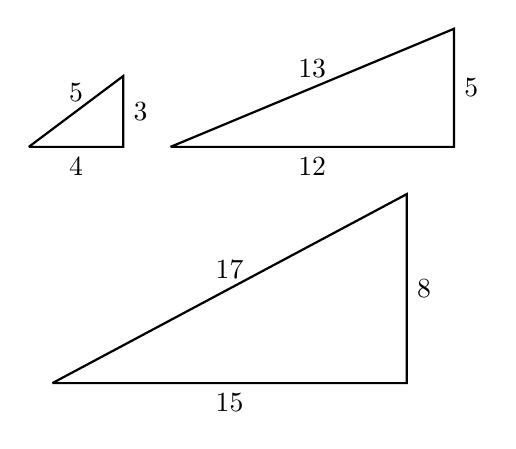
\begin{tikzpicture}[thick, scale=0.30]
        \draw (0,0) -- (4,0) node[midway,below]{$4$}
        -- (4,3) node[midway,right]{$3$}
        -- (0,0) node[midway,above]{$5$};
        \draw (6,0) -- (18,0) node[midway,below]{$12$}
        -- (18,5) node[midway,right]{$5$}
        -- (6,0) node[midway,above]{$13$};
        \draw (1,-10) -- (16,-10) node[midway,below]{$15$}
        -- (16,-2) node[midway,right]{$8$}
        -- (1,-10) node[midway,above]{$17$};
    \end{tikzpicture}
\end{center}

我们是怎么知道的呢?这是一个非常有用的事实,你可能在数学课上(或者生活中不经意地)用过很多次。你有没有思考过为什么这是真的?你会如何向持怀疑态度的朋友解释呢?这就是\textbf{数学证明}试图完成的:对事实的清晰简洁的解释。要求证明背后的原因也十分有意义,它具有两重含义:确信我们认为是真的事情确实真的,并且要使用时不必每次都其进行解释。在(令人满意地)证明毕达哥拉斯定理之后,我们只需在相关情况出现时通过名字引用该定理即可;我们已经证明过了,所以无需再次证明。

那么,究竟什么构成了证明?怎么知道解释是否足够清晰和简洁?一般来说,回答这个问题相当困难,这也是为什么数学既可以被视为科学,也可以被视为艺术的部分原因。没错,我们处理的都是冰冷艰涩的事实,但能够对这些事实进行推理并向他人以令人满意的形式解释清楚,这本身就是一种艺术。

\subsubsection*{“证明”范例}

让我们一起看几个“证明”的例子,看看它们是否足够好。(我们现在先说“证明”,稍后为其下更精确的定义。)这里是第一个:

\begin{proofs}{“证明” 1.}
    画一个边长为 $a+b$ 的正方形。在这个正方形里画 $4$ 个相同的直角三角形,这 $4$ 个直角三角形在大正方形的内部组成一个边长为 $c$ 的正方形。

    \begin{center}
        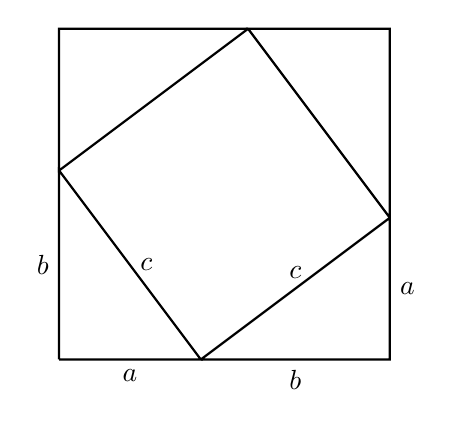
\begin{tikzpicture}[thick, scale=0.6]
            \draw (0,0) -- (3,0) node[midway,below]{$a$}
            -- (0,4) node[midway,right]{$c$}
            -- (0,0) node[midway,left]{$b$};
            \draw (3,0) -- (7,0) node[midway,below]{$b$}
            -- (7,3) node[midway,right]{$a$}
            -- (3,0) node[midway,above]{$c$};
            \draw (7,3) -- (7,7)
            -- (4,7)
            -- (7,3);
            \draw (4,7) -- (0,7)
            -- (0,4)
            -- (4,7);
        \end{tikzpicture}
    \end{center}

    大正方形的面积可以用两种方式表示:应用正方形的面积公式,或者把小正方形和四个三角形的面积加起来。因此,下面这个等式一定成立。
    \[(a+b)^2=c^2+4\cdot\frac{ab}{2}=c^2+2ab\] 
    将左边表达式展开,然后两边同时消掉同类项可得 
    \[a^2+\cancel{2ab}+b^2=c^2+\cancel{2ab}\] 
    所以,$a^2+b^2=c^2$ 成立。
\end{proofs}

上面的证明能说服你吗?每一步都合理吗?可能你现在还不确定,所以让我们看一下此定理的另外一种“证明”。

\begin{proofs}{“证明” 2.}
    假设毕达哥拉斯定义成立,绘制直角三角形,并过直角对应的顶点做高。如下图所示标记点和边长:
    \begin{center}
        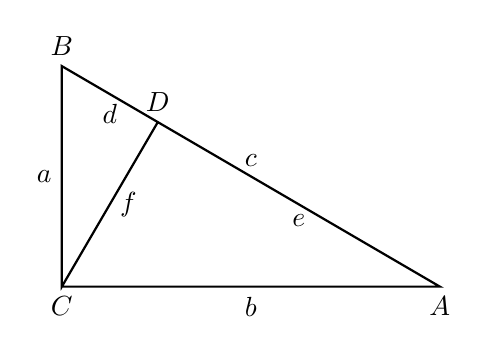
\begin{tikzpicture}[thick, scale=0.8]
            \coordinate (C) at (0,0);
            \coordinate (A) at (6,0);
            \coordinate (B) at (0,3.5);
            \coordinate (D) at (1.523316, 2.611399);
            \draw (C) node[anchor=north]{$C$}
            -- (A) node[anchor=north]{$A$} node[midway,below]{$b$} 
            -- (B) node[anchor=south]{$B$} node[midway,above]{$c$}
            -- (C) node[midway,left]{$a$}
            -- (D) node[anchor=south]{$D$} node[midway,right]{$f$}
            -- (A) node[midway,below]{$e$} 
            -- (D)
            -- (B) node[midway,below]{$d$};
            \rightAngle{B}{D}{C}{0.3};
        \end{tikzpicture}
    \end{center}
    因为毕达哥拉斯定理成立,所以我们可以将其应用到图中的三个直角三角形中,即三角形 $ABC, BCD, ACD$。(定义 $e = c-d$)可得
    \begin{align*}
        a^2 &= d^2 + f^2 \\
        b^2 &= f^2 + e^2 \\
        c^2 &= a^2 + b^2
    \end{align*}
    将前两个方程相加再用第三个方程替换,可得
    \[c^2 = d^2 + e^2 +2f^2\]
    请注意,角 $\angle ABC$ 和 $\angle ACD$ 相等,因为它们都与角 $\angle CAB$ 互补,因此我们知道三角形 $\triangle CDB$ 和 $\triangle ADC$ 是相似三角形。(这里假设你对平面有一定了解。)由此可得 $\frac{e}{f} = \frac{f}{d}$,因此 $f^2 = ed$。我们可以将其带入上面的公式替换 $f^2$,结果如下:
    \[c^2 = d^2+e^2+2de = (d+e)^2\]
    两边同时开方(已知 $c,d,e$ 都是正数)可得 $c = d+e$,根据边长 $d$ 和 $e$ 的定义,这显然成立。因此,假设毕达哥拉斯定理成立是正确的。
\end{proofs}

这个证明怎么样?有说服力吗?清楚吗?在我们确定什么构成“正确的”或“良好的”证明之前,让我们再检验一个“证明”。

\begin{proofs}{“证明” 3.}
    观察下图
    \begin{center}
        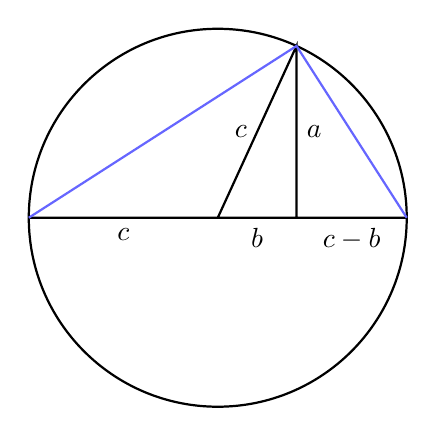
\begin{tikzpicture}[thick, scale=0.4]
            \coordinate (O) at (0,0);
            \coordinate (A) at (-6,0);
            \coordinate (B) at (6,0);
            \coordinate (C) at (2.5,0);
            \coordinate (D) at (2.5,5.45435);
            \draw (O) circle (6);
            \draw (A) -- (O) node[midway,below]{$c$}
            -- (C) node[midway,below]{$b$}
            -- (B) node[midway,below]{$c-b$}
            -- (C)
            -- (D) node[midway,right]{$a$}
            -- (O) node[midway,left]{$c$};
            \draw[color=blue!60] (A) -- (D) -- (B);
            \rightAngle{B}{C}{D}{0.6};
        \end{tikzpicture}
    \end{center}  
    易得 $\frac{a}{b+c} = \frac{c-b}{a}$,因此 $a^2 + b^2 = c^2$。
\end{proofs}

这个证明对你来合理吗?最后,还有一个需要思考的“证明”。

\begin{proofs}{“证明” 4.}
    毕达哥拉斯定理一定成立,否则我的老师就一直在骗我。
\end{proofs} 

\subsubsection*{讨论}

在继续阅读之前,我们鼓励你先思考一下这四个“证明”,甚至与同学或朋友讨论一下。你认为什么构成“正确”的证明?清晰性和易读性重要吗?它会影响证明的“正确性”吗?

从历史的角度来看,数学证明的撰写已经发展了多年,并且对于什么构成“正确”的证明存在良好的普遍共识:

\begin{itemize}
    \item 从数学角度来说,证明中的每一\textit{步}、每一个逻辑推论和主张都是\textit{有效的},这一点很重要。
    \item 同样重要的是,证明撰写者必须(合理地)明确为什么某个陈述来自先前的工作或外部知识。
\end{itemize}

\textit{真理}的这些要求的好处在于,一旦数学已经建立起来,我们就可以通读一个论证并验证每个主张是\textbf{对}还是\textbf{错}。难以定义的是清晰的写作。在某种程度上,这很像最高法院法官波特·斯图尔特(Justice Potter Stewart)对淫秽的著名定义:“当我看到它时,我就知道”。

让我们对给出的四个论证进行比较,评估它们的清晰性和正确性:

\textbf{清晰性:}

\begin{itemize}
    \item “证明”1和“证明”2已经解释得非常清晰。对于作者在做什么以及为什么这样做有明确的阐述。他们指出了每个程式的来源,甚至还包含一些图片来向读者说明他们的想法。
    
    请注意,“证明 1”确实依赖于一些基本的先验知识,例如变量的代数运算以及三角形和正方形面积公式,但这没有问题。

    同样地,“证明 2”依赖于对相似三角形的一些理解以及它们边长之间的关系。至少撰写者指出了这一点,所以有兴趣的读者可以查阅先关知识点。如果撰写者不给,读者可能会感到困惑,不知道如何得出这个结论。
    \item “证明”3写得非常糟糕!它没有提供任何解释。这使得很难确定其说法是否真正正确。没错,其中包括一张图片,但没有说明\textit{为什么}会选择在三角形周围画一个圆,或者为什么从图中得出所述方程。
    \item “证明”4是一个语法正确的句子,但它并不能\textit{解释}任何事情!
\end{itemize}

我们已经可以看到,“证明”4无疑不是一个良好且正确的证明的可行候选者。“证明”1和“证明”2仍在候选之列,因为它们至少写得很清楚。“证明”3目前看可能不是一个好的候选者;然而,也许它确实包含正确的结论,只是需要更好的解释。也许它可以被重写为一个恰到好处的\textit{证明}。

让我们再来分析一下这四个论证的逻辑正确性:

\textbf{正确性:}

\begin{itemize}
    \item “证明”1大部分都很好。正确应用了正方形和三角形面积的公式,并且其代数运算也正确。但是我们怎么知道其描述的过程 --- 将给定三角形的四个副本放入一个更大的正方形内 --- 会构建一个内部边长为 $c$ 的正方形?证明中只是说这样\textit{可以},但并没有真正说明\textit{为什么可以}。不过,除了这个疏漏外,这个证明写得很好而且是正确的。
    
    (你能证明里面的形状实际上是正方形吗?看一下它的角度:你能说明为什么它们都是直角吗?)
    \item 不幸的是,“证明”2完全是错的!它所做的每一个逻辑步骤都遵循前一个步骤。例如,假设我们以这种方式设置三角形,我们可以正确推断出 $\triangle CDB$ 和 $\triangle ADC$ 是相似三角形。然而,为什么我们可以在一开始就\textit{假设}该定理为\textbf{真}呢?总的来说,这不正是我们在证明中试图实现的目标吗?这是一个关键缺陷。\textbf{假设一个事实并从中推断出一些结论为真并不能让我们得出原始假设是有效的结论。}
    
    如果这种方法有效,我们就可以“证明”我们想要的任何东西!举个例子:你如何看待以下证明 $0 = 1$ 的“证明”?
    \begin{proof}
        假设 $0 = 1$。那么,根据 $=$ 的对称性,$1 = 0$ 也是成立的。将这两个方程相加可得 $1 = 1$,这显然为真。因此,$0 = 1$ 是一个有效的假设,因此它一定为真。
    \end{proof}
    你看出上面证明与“证明”2有什么相似之处吗?使用了同样有缺陷的推理:我们假设一个事实,做了一些工作以得到我们知道为真的其他事实,然后说假设的事实也必须为真。
    \item 对于“证明”3,大多数数学家会说这是一个“糟糕的证明”,尽管事实上它表现出的一切声明似乎都是正确的。我们说“表现出”是因为,如果没有任何词语来解释发生了什么,我们实际上不知道撰写者想说什么!然而,我们会说,完美证明的核心就包含在其中。
    
    从图中,你可以证明方程 $\frac{a}{c+b} = \frac{c-b}{a}$ 一定成立。(提示:使用相似三角形!)从这开始,通过一个简单的操作就可以推断出 $a^2 + b^2 = c^2$。

    你能写一些文字来配合图表,将其变成得当的证明吗?
    \item 最后,几乎每个逻辑正常的人(我们希望如此!)都会说“证明”4 根本不是一个证明,无论做出这样的陈述多么方便。
\end{itemize}

上述讨论表明“证明”1 实际上是一个好的证明。4个证明中,“证明”1 写得最清楚,逻辑也最正确。我们现在可以将其作为\textbf{证明}。“证明”2 是完全错误的,尽管它表述得非常清楚。“证明”3 包含正确的想法,但缺乏明确的表达。“证明”4 离证明十万八千里,我们甚至不想讨论它。

\subsubsection*{问题}

在继续讨论其他主题之前,留个问题给你:如果给你三个正数 $a,b,c$ 满足 $a^2+b^2=c^2$,是否一定存在边长为 $a,b$ 斜边长为 $c$ 的直角三角形?如果存在,你会如何着手构建它?如果不存在,为什么不存在?

\subsection{质数时间}\label{sec:section1.1.2}

当我们讨论证明这个主题时,让我们看一下另一个不同定理的证明。作为提醒(或简要介绍),我们来谈谈\textit{质数}。

\subsubsection*{定义、示例和使用}

\begin{definition}\label{def:prime}
    如果大于 $1$ 的正整数 $p$ 其正因子只有 $1$ 和 $p$,则称 $p$ 为\textbf{质数}。非质正整数称为\textbf{合数}。
\end{definition}

质数已被证明在数学的所有分支中都非常重要,而不仅仅是对整数及其性质的研究,即\textbf{数论}。数学中最著名的\textbf{猜想}(迄今为止既没有被证明也没有被证伪的定理的猜测)当数\textit{黎曼猜想}。其结论已被证明与全体整数中质数的分布密切相关。围绕这个主题已经写了很多书。此外,大多数现代密码学都是基于将巨大质数相乘,因为它们的乘积很难逆向分解为两个巨大质数因子。现在你知道了:每次你用信用卡在 iTunes 上购买歌曲时,某些计算机都会将两个大质数相乘!

前几个质数是 $2, 3, 5, 7, 11, 13, 17, 19, 23,\dots$(记住,$1$ 不满足定义)。质数有多少个?他们相距多远?存在模式吗?回答这些问题可能很有趣,但也很困难(有时甚至是不可能的!)。这里,我们将回答其中一个问题:质数是否有无穷多个?

\subsubsection*{定理和证明}

\begin{theorem}[质数无限性]
    质数有无穷多个。
\end{theorem}

\begin{proof}
    假设质数有有限多个,并按升序列出:$p_1, p_2, p_3, \dots, p_k$,所以 $p_k$ 是所有质数中最大的。定义新数
    \[N = (p_1 \cdot p_2 \cdot p_3 \cdot \dots \cdot p_k) + 1\]
    $N$ 一定能被某个质数整除。然而,它一定不能被 $p_1$ 或 $p_2$ 或 $\dots$ 或 $p_k$ 整除,因为根据 $N$ 的定义都会有余数 $1$。因此 $N$ 可以被列表中未列出的其他质数整除。

    如果 $N$ 本身是合数(即不是质数),那么我们就发现了一些新质数 $p < N$,它不在我们的所有质数列表中。如果 $N$ 本身是质数,那么我们就有了一个新质数 $N > p_k$,所以 $p_k$ 实际上并不是最大的质数。不管哪种情况,我们保证有一个新的质数不会出现在给定的 $k$ 个质数列表中。因此,质数必定有无穷多个。
\end{proof}

对于这个“证明”你怎么看?你确信吗?感觉与我们迄今为止看到的其他论证有点不同,不是吗?尝试向同学解释这个证明与上一节毕达哥拉斯定理的“证明 1”有何不同。我们很快将揭示:这里的“证明”实际上是一个完全正确的\textit{证明},没有引号!
    
\subsection{无理数的傲慢}

现在让我们讨论另一种类型的数字:\textbf{有理}数。你可能知道“分数”、“商”或“比率”都是有理数。

\subsubsection*{定义和示例}

下面是\textit{有理}数的精确定义:

\begin{definition}
    实数 $r$ 是\textbf{有理}数当且仅当它可以表示为两个整数之比 $r = \frac{a}{b}$,其中 $a$ 和 $b$ 都是整数(且 $b \ne 0$)。

    一个实数不是有理数就是\textbf{无理数}。
\end{definition}

这个定义中没有任何内容表明有理数必须只有一种定义中的表示形式;它只要求有理数至少有一种定义中的表示。例如,$1.5$ 是有理数因为 $1.5 = \frac{3}{2} = \frac{12}{8} = \frac{30}{20}$ 等等。一个实数不是有理数就是\textbf{无理}数,这就是完整定义:\textit{非}有理数,即不存在将数字表示为整数之比的形式。你可能知道 $\sqrt{2}$ 是一个无理数,但你要如何\textit{证明}这一点呢?自己尝试证明一下。我们稍后会重新审视这个问题(见4.9.4)。其他你可能知道的无理数还包括 $e, \pi, \varphi$ 和 $\sqrt{n}$,其中 $n$ 为正整数且不为完全平方数。

\subsubsection*{问题}

给定有理数/无理数的定义,我们可能想知道如何组合无理数来产生有理数。尝试自己回答以下问题。如果你的答案为“是”,请尝试找到一个例子,如果你的答案为“否”,请尝试解释为什么要求的情况不可能实现。

\begin{enumerate}
    \item 是否存在无理数 $a$ 和 $b$ 使得 $a \cdot b$ 为有理数?
    \item 是否存在无理数 $a$ 和 $b$ 使得 $a + b$ 为有理数?
    \item 是否存在无理数 $a$ 和 $b$ 使得 $a^b$ 为有理数?
\end{enumerate}

你能找出例子吗?事实证明,这三个问题的答案都是“是”!前两个不太难理解,但第三个有点棘手。

这里,我们给出证明来证明第三个问题的答案为“是”。有趣的是,我们实际上不会给出满足 $a^b$ 为有理数的 $a$ 和 $b$ 的确切数字;我们只是将其范围缩小到两种可能的选择,并证明其中任意一种选择\textit{必定}有效。听起来很有趣,对吧?我们来试试吧。

\begin{proof}
    我们知道 $\sqrt{2}$ 为无理数。考虑数字 $x = \sqrt{2}^{\sqrt{2}}$。有两种可能的情况:
    \begin{itemize}
        \item 如果 $x$ 为有理数,那么我们可以令 $a = \sqrt{2}, b = \sqrt{2}$ 即可得到答案。
        \item 如果 $x$ 为无理数,那么我们可以令 $a = \sqrt{2}^{\sqrt{2}}, b = \sqrt{2}$,则
        \[a^b = \Bigg(\sqrt{2}^{\sqrt{2}}\Bigg)^{\sqrt{2}} = \Big(\sqrt{2}\Big)^{\sqrt{2} \cdot \sqrt{2}} = \Big(\sqrt{2}\Big)^2 = 2\]
        $2$ 为有理数。
    \end{itemize}
    任意一种情况,我们都能找到无理数 $a$ 和 $b$ 使得 $a^b$ 为有理数。因此,这样的数字对一定存在。
\end{proof}

你觉得这个证明怎么样?有说服力吗?它以明确的“是”回答了上面的第三个问题,但它并没有告诉我们\textit{哪}一对 $a, b$ 实际上是正确的,而只是告诉我们其中有一对有效。(事实证明 $\sqrt{2}^{\sqrt{2}}$ 也是无理数,但这一事实需要更多的工作来证明。)

还有很多其他具体例子可以回答这个问题。你能想出任何其他方法吗?(提示:尝试使用 $\log_{10}$ 函数...)


\newpage
% !TeX root = ../../book.tex
\section{博览会展览}\label{sec:section1.2}

\subsection{简单符号}

\subsubsection*{数学是门语言}

尽管看上去全是符号(以及那些写得密密麻麻的教科书所呈现的),但数学不仅仅是我们在纸上使用的符号的集合。英语基于一组固定的符号(字母表中的 26 个字母加上常见的标点符号,如句点、逗号和括号),而我们以特定的方式将这些符号组合在一起,并遵循一定的标准和约定,创作出有意义的单词、短语、句子、段落等;从本质上讲,英语与任何其他语言一样,通过符号集合以及组织这些符号的规则的集合,来传达含义。同样的概念也适用于\textit{数学语言}:有一组符号和一组作用于这些符号的规则。

一个区别是,我们在数学中使用的符号集合可能相当大,具体取决于当前讨论的数学分支。数学结构多样性的一个重要部分是我们总是可以创建和定义要使用的新符号。通常,这样做只是为了使内容更简短、更易于阅读。

数学与其他语言之间的另一个主要区别是,我们仔细选择如何\textit{定义}我们的单词及其表达的概念。通常,数学家的大多数争论都围绕定义展开。这可能会令你感到惊讶;似乎数学家就证明和猜想进行辩论才更合理,甚至数学家居然会辩论都是一个新奇的想法!为新发现的概念选择正确的定义和术语是数学发现和阐述的重要组成部分,因为这有助于发现者/发明者向其他感兴趣的人解释他/她的想法。(没有这个过程,数学就不会进步,只是一群孤立的人试图自己发现真理。)

口语的情况与此类似,但似乎没有那么极端。例如,如果你对你的朋友说,“我饿了”,或者“我感觉有点饿了”,或者“天哪,我饿死了”,他们听到的基本上是相同的信息,并给出大致相同的回应。然而,在数学中,我们的定义要精确得多,并且不包含口语允许的细微差别。当然,这两种哲学各有优缺点,但在数学中,我们尽可能追求精确,因此我们希望我们的定义准确且稳定。尽管如此,我们可以掌控这些定义是什么!这就是为什么关于定义的争论在数学世界中如此普遍:为手头的概念选择正确的定义可以使未来使用这些概念的工作变得更加容易和方便。

\subsubsection*{恰当选择定义}

作为一个具体的例子,让我们回到上一节中看到的质数的定义\ref{def:prime}。它说的是:

\begin{definition}
    如果大于 $1$ 的正整数 $p$ 其正因子只有 $1$ 和 $p$,则称 $p$ 为\textbf{质数}。非质正整数称为\textbf{合数}。
\end{definition}

这个定义似乎没有什么问题,不是吗?也许你会用不同的措辞或更简洁的表达或使用不同的可变字母或其他,但最终的信息是相同的:质数是具有特定属性的某种类型的数字。而你选择写出该特定类型的数字是什么(大于 $1$ 的正整数)以及该属性是什么(没有除 $1$ 和它本身以外的正因子),你将获得等效的定义。

不过,这个定义背后存在一些微妙的问题:为什么它是那种特定类型的数字?为什么我们如此关心这个特殊的属性 --- 只能被 $1$ 和它本身整除?如果定义略有不同怎么办?事情真的会有那么大的改变吗?我们将用另一个问题来解决这些问题:你如何看待以下质数的替代定义?

\begin{definition}\label{def:prime2}
    如果小于 $-1$ 或大于 $1$ 的整数 $p$ 其正因子只有 $1$ 和 $p$,则称 $p$ 为\textbf{质数}。
\end{definition}

你注意到细微的差别了吗?所有符合之前“质数”定义的数字仍然符合这个定义,但现在负数也适用!具体来说,给定任意数字 $p$ 在旧定义下是质数,$-p$ 现在在新定义下也是质数。这是一个合理的想法吗?负质数有什么问题?

质数的第三个定义怎么样?

\begin{definition}\label{def:prime3}
    如果正整数 $p$ 的正因子只有 $1$ 和 $p$,则称 $p$ 为\textbf{质数}。
\end{definition}

(请记住,按照惯例,$0$ 既不是正数也不是负数。)现在,负数会超出范围,但 $1$ 符合此定义。这合理吗? $1$ 的唯一正因子是 $1$ 和...它本身,对吗?

这就是可能引发争论的地方:也许你不介意让 $1$ 成为质数,但你的朋友会强烈反对。好吧,如果没有确凿的理由,就没有办法说你们中任何一个都是错的,真的;你只是对术语做了不同的选择,它们都没有改变 $1$ 的唯一正因子是 $1$ 和它本身这一固有属性。类似地,请考虑一下:无论你称它们为凉鞋、拖鞋还是人字拖,事实仍然是这些类型的鞋子适合在海滩上穿。

然而,考虑到历史的后见之明和新的愿望,通常一个特定的定义被认为更加合适。未来,我们将研究质数分解,这是一种将每个(正)整数写为质数乘积的方法。例如,$15 = 3 \cdot 5$, $12 = 2 \cdot 2 \cdot 3 = 2^2 \cdot 3$ 和 $142857 = 33 \cdot 11 \cdot 13 \cdot 37$ 都是质因数分解。

这些因数分解也有一个特殊的性质:一般来说,正整数的质因数分解是\textbf{唯一的}!也就是说,只有一种方法可以将正整数写为质数的乘积(因为我们将因子的不同排序视为同一事物,所以 $105 = 3 \cdot 5 \cdot 7$ 和 $105 = 7 \cdot 3 \cdot 5$ 是相同的因数分解)。我们将使用上面给出的第一个定义严格证明这一点。如果我们使用第二个定义或第三个定义会怎么样?这种唯一性还存在吗? 为什么这种唯一性如此重要?最终,结论是,定义应该由逻辑和实用性驱动,并且这可能会随着时间的推移而改变并引发一些争论。

\subsubsection*{数学家的学习模式}

建立清晰准确的定义的另一个好处是你可以像思想者一样获取知识和理解;人类学习的一个主要方面涉及通过日常经验识别模式,接着将想法、概念、词语、事件与这些模式联系起来。然后,人们可以使用这些模式来预测抽象的想法、概念和事件并对其进行理论化。

例如,研究表明,人类婴儿最初缺乏\textit{物体存继性}概念,随着时间的推移逐渐发展起来。如果你给孩子看一个他们喜欢的彩色玩具,然后把它藏在纸箱下面,孩子不太明白这个玩具仍然存在,只是看不见了。他/她会表现得好像该物体不再存在一样。然而,在某些时候,我们知道这不是真的,我们视野之外的物体仍然存在。这究竟是如何发生的?也许是我们见识到许多此类事件的模式,其中一个物体“消失”,然后我们又找到它。

更好的例子可以在自然科学中找到,它们说明了模式识别和抽象思维的另一个方面,这是极其重要的,特别是在数学和科学领域。我们可以想象,尼安德特人不知何故知道,每当他们拿起一块岩石并将其保持在一定距离,然后松开时,岩石就会掉到地上。这种情况可能一次又一次地发生,所以他们“明白”这种现象是自然的必然产物。在发生足够多的事件之后,人们很可能明白这种情况总会发生,或者至少,任何没有发生的情况都会引起极大的困惑和恐惧。(正是这种情绪反应可能有助于解释火山爆发等罕见但强烈的事件如何导致古代文明将此类事件归咎于“神之愤怒”)。

对事件的观察并没有使史前人类进一步理解\textit{为什么}岩石总是会掉落到地面,或者能够\textit{解释}为什么它每次都必然发生。几千年后,人们才开始思考这种现象为何发生以及如何发生,更长时间之后,艾萨克·牛顿(Isaac Newton)最终提出了一个试图解释重力行为的模型(最终为此类现象命名)。有人说,即使是现在,我们仍然没有弄清楚它到底是如何运行的。(如果你好奇的话,可以上网搜索“循环量子引力”并尝试理解这一点)。

正是这种思维上的抽象飞跃 --- 从对某种模式的观察到对该模式的认识论理解 --- 从最好的意义上来说,是真正具有好奇心和智慧的思想家、真正的科学家的特征。你认为谁是更好的昆虫学家:贪婪的读者,他已经记住了世界上所有目前已知的甲虫种类,或者实验室科学家,他检查了多种物种,可以采集新标本并对其分类为甲虫还是非甲虫?这在某种程度上是一个引导性问题,但要点是:\textit{理解}定义及其背后的动机比简单地了解一堆满足某个定义的\textit{实例}要有益得多。

可以说,这对数学更为重要。你能想象一个数学家不知道质数是什么,只能凭记忆列出前 100 个质数并对此沾沾自喜吗?当然不是!数学研究的美妙、通用和魅力部分在于我们检查模式和现象,然后选择如何做出与这些模式相关的适当定义。然后,我们利用对这些模式的新理解来对其他模式和现象做出严格精确的预测。彻底理解定义或概念可以提高预测能力,并且比仅仅了解该定义/概念的示例更为有效。


\subsection{书写正确}

数学的另一个有趣的方面是,尽管它本身就是一种语言,但我们依赖外部语言来传达我们所拥有的数学思想和见解。尝试在不使用任何单词的情况下重写我们之前看过的定义和证明。这很难,不是吗?因此,我们希望用来传达数学思想的书面语言遵循与我们所写的数学“句子”相同的标准:我们希望它们\textit{精确}、\textit{合乎逻辑}且\textit{清晰}。

现在,为这三个词下一个精确、合乎逻辑且清晰的定义本身就是一项艰巨的任务。然而,我们都认同理想的证明应该是:

\begin{itemize}
    \item \textbf{精确的:}任何个体陈述都不应是不真实的或可以通过多种方式解释从而导致真相需要商榷;
    \item \textbf{合乎逻辑的:}每一步都应遵循先前的步骤,并有适当的动机和解释;
    \item \textbf{清晰的:}步骤间应该用正确的语法连接和描述,帮助读者了解发生了什么。
\end{itemize}

让我们检视几个无视这些标准并且在某种程度上不符合我们迄今为止的证明定义的“证明”。

\subsubsection*{糟糕“证明” \#1}

首先,我们来一个 $1=2$ 的“证明”,我们知道这肯定有问题。你能找到哪里出错了吗?它违反了哪个标准?精确、合乎逻辑还是清晰?

\begin{proofs}{“证明”}
    假设有两个实数 $x$ 和 $y$,考虑如下等式:
    \begin{align*}
        x &= y \\
        x^2 &= xy &\text{两边同时乘以} y\\
        x^2-y^2 &= xy-y^2 &\text{两边同时减去} y^2\\
        (x+y)(x-y) &= y(x-y) &\text{因式分解} \\
        x + y &= y &\text{两边同时消掉} (x-y)\\
        y + y &= y &\text{因为第一行给定} x=y\\ 
        2y &= y \\
        2 &= 1 &\text{两边同时除以} y
    \end{align*}
\end{proofs}

这里的问题是\textit{精确}。对第四行进行因式分解后,除以公因数 $(x - y)$ 即可得到第五行,这似乎既方便又明智;然而,第一行告诉我们 $x = y$,所以 $x-y = 0$,\textbf{除以零是不允许的}!使用变量 $x$ 和 $y$ 只是一种让你失去踪迹并掩盖除以零的方法。(说到这里,为什么不能除以零?你能想出一个合理的解释吗?从乘法的角度思考一下。)

\subsubsection*{糟糕“证明” \#2}

这是类似“事实”的另一个证明,即 $0 = 36$。

\begin{proofs}{“证明”}
    考虑方程 $x^2+y^2 = 25$。整理并分离 $x$ 可得
    \[x = \sqrt{25-y^2}\]
    两边加3再同时平方得
    \[(x+3)^2=\Big(3+\sqrt{25-y^2}\Big)^2\]
    请注意,$x = -3$ 和 $y = 4$ 是原方程的解,所以最终的方程也应该是成立的。将这组解代入 $x$ 和 $y$ 可得
    \[0 = (-3+3)^2 = (3+\sqrt{25-16})^2 = (3+3)^2 = 36\]
    因此,$0 = 36$。
\end{proofs}

到底发生了什么?你能发现不合逻辑的步骤吗?如果我们使用最后选择的变量 $x$ 和 $y$ 的特定值重写证明步骤,也许会有所帮助:

\begin{align*}
    (-3)^2+4^2 &= 25 \\
    -3 &= \sqrt{25-4^2} \\
    (-3+3)^2 &= \Big(3+\sqrt{25-4^2}\Big)^2 \\
    0 &= 36
\end{align*}

现在很明显了,不是吗?对方程两边进行平方根运算存在一个问题,它取决于 $(-x)^2=x^2$ 这一事实。

当我们解 $z^2=x^2$ 这样的方程时,必须牢记这个方程有两个根:$z = -x$ 和 $z = x$。因此,从方程开始并对两边进行平方是一个完全合乎逻辑的步骤(所得方程的真值与原方程的真值\textit{一致}),但反之却是一个不合逻辑的步骤(平方方程成立并不\textit{一定}等于平方根方程也成立)。这是一个带有\textbf{条件语句}或\textbf{逻辑蕴涵}的问题,我们稍后会详细讨论这些概念(第 4.5.3 节)。现在,我们可以用下面的代码来总结这个概念:

\[\text{如果} a=b, \text{则} a^2=b^2, \text{反过来,如果} a^2=b^2, \text{则} a=b \text{或} a=-b\]

这说明了为什么在上面“证明”中从 $x^2+y^2 = 25$ 到 $x = \sqrt{25-y^2}$ 这步是不合逻辑的:当有两种可能的选择时,我们立即假设平方根的一种特定选择。如果我们选择负平方根,会发生什么?试着将第二步替换为 $-x = \sqrt{25-y^2}$ 并重写证明,在最后对 $x$ 和 $y$ 使用相同的值。发生了什么? 如果你用 $x = 3, y = -4$ 代替呢?或者 $x=-5, y=0$ 呢?你能描述一下如何确定何时应该使用正根 $x$ 何时应该使用负根 $-x$ 吗?

\subsubsection*{数学使用“包含或”}

既然“或”这个词已经出现,我们先提一下上面句子中\textit{或}的使用。当我们说 “$a = b$ 或 $a = -b$” 时,我们的意思是,这两个陈述中\textit{至少}有一个必须为真,甚至可能两者都为真。现在,如果 $a \ne 0$ 且 $b \ne 0$,则只有其中一种结论性陈述可以为真;也就是说,在这种情况下,只有一个根(正或负)是正确的,而不是两者都是正确的。然而,如果 $b = 0$,那么两个结论性陈述说的是同样的事情,$a = 0$,因此规定\textit{或}意味着只有一个陈述可以为真并且不允许它们都为真,这是不合逻辑的。在其他情况下,这种区别会产生更显着的差异。

例如,如果你在餐厅点了一份三明治,服务员问:“您想要薯条还是土豆沙拉?”,这可以理解为,你可以选择其中一项,但不能同时选择两者。这就是\textbf{异或}的示例,因为它阻止你选择两个选项。或者,如果你忘记带书写工具去课堂,准备用老方法记笔记于是询问你的朋友,“我可以借用您的铅笔或钢笔吗?”,这可以理解为,你实际上并不关心提供两个选项中的哪一个,只要至少有一个可用即可。也许你的朋友两者都有,而且其中任何一个都可以。这是\textbf{包含或}的示例,并且这是所有数学示例中假定的解释。

\subsubsection*{不清楚的论证}

最后两个糟糕的“证明”问题在于精确性和逻辑正确性。我们要求良好证明的第三个条件是\textit{清晰}:我们希望文字能够解释证明者在每个步骤中完成的工作以及为什么该工作是相关的。换句话说,我们不希望读者在任何时候停下来问:“这句话是什么意思?”或“那是从哪里来的?”或因困惑而产生的类似问题。如果有帮助的话,考虑写一个证明,向你班上的朋友、将要阅读你作业的评分者或智力相当的家庭成员解释它。重读你自己写的证明,并尝试预测可能出现的问题或可能要求你进行的澄清,然后通过重写来解决这些问题。

证明可能因为多种原因失败或不清晰,首当其冲的是,单词和句子可能无法正确解释证明的步骤和动机,这实际上可能是因为单词太多(使读者负担过重而模糊了证明)或因为单词太少(没有给读到者足够的信息)或者因为所选的词语令人困惑(没有正确解释证明)。这些是证明\textit{语言}的问题。

从数学上讲,就清晰性而言,可能会出现许多问题。也许证明撰写者突然引入一个变量,但没有说明它是什么类型的数字(整数、实数等),或者跳过几个算术/代数步骤,或者使用新的符号而没有提前定义它的含义...这些行为在技术上都没有错误或不合逻辑,但它们肯定会给读者带来困惑。你能想到其他原因让证明不明确吗?尝试想出一种基于语言的原因和一种基于数学的原因。

\subsubsection*{糟糕“证明” \#3}

让我们陈述一个关于多项式函数的简单事实,然后查阅关于该事实的“证明”。仔细阅读论证并尝试找出一些不清楚的句子或数学步骤。

\textbf{事实:}考虑多项式函数 $f(x) = x^4-8x^2+16$。对于任意 $x$,该函数都满足 $f(x) \ge 0$。

\begin{proofs}{“证明”}
    无论 $x$ 的值是多少,我们将其代入 $x$ 的函数 $f$ 中,都可以通过对多项式进行因式分解写出该函数的输出值,如下所示:
    \[f(x) = x^4-8x^2+16 = (x-2)^2(x+2)^2\]
    而任意数字 $z$ 一定要么小于 $-2$,要么大于 $2$,要么严格介于 $-2$ 和 $2$ 之间,要么等于其中之一。当 $z > 2$ 时, $z - 2$ 和 $z + 2$ 都大于 $0$,因此 $f(z) > 0$。当 $z < -2$ 时,两项都为负而负数的平方为正,所以 $f(z) > 0$。当 $-2 < z < 2$ 时,类似情况再次发生,当 $x = 2$ 或 $x = -2$ 时,其中一项为 $0$,所以 $f = 0$。因此,我们要证明的必然成立。
\end{proofs}

这个证明有什么可批评的地方呢?首先,它正确吗?精确吗?符合逻辑吗?清楚吗?哪里不清楚?试着找出那些有点不清楚的陈述,无论是语言上的还是数学上的,并尝试适当地修改它们。在不指出个别错误的情况下,下面提供了上述事实的更好、更清晰的论证。

\begin{proof}
    我们首先对函数 $f(x)$ 进行因式分解,将其视为变量为 $x^2$ 的二次函数
    \[f(x) = (x^2)^2-8x^2+16 = (x^2-4)^2\]
    接下来,我们可以因式分解 $x^2-4=(x+2)(x-2)$ 并将原函数重写为
    \[f(x) = \big((x+2)(x-2)\big)^2 = (x+2)^2(x-2)^2\]
    对于任意实数 $x$,都有 $(x+2)^2 \ge 0$ 且 $(x-2)^2 \ge 0$,因为平方结果一定非负。两个非负项的成绩依然非负,所以 对于任意实数 $x$, $f(x) = (x+2)^2(x-2)^2 \ge 0$。
\end{proof}

第一个“证明”和第二个“证明”有什么区别?你重写的证明也像第二个证明吗?

对第一个“证明”的批评之一是它没有完全解释 $-2 < x < 2$ 的情况;相反,它只是说发生了“类似”的事情,并没有实际执行任何细节。这是数学中的常见情况(证明的某些步骤“留给读者”),这是一种简便技巧,有时可以避免繁琐的算术/代数,并使阅读证明更容易、更快速、更愉悦。但是,要谨慎使用该技巧。作为证明撰写者,确保步骤确实有效非常重要,即使你不打算在证明中呈现它们;你应该向读者提供简短的摘要或提示,说明这些步骤实际上是如何运作的。此外,证明撰写者应尽量不要在对证明最终结果至关重要的步骤上使用此技巧。

在上面的特例中,完全跳过了因式分解的实际步骤,并且只是顺便提及了对 $-2 < x < 2$ 情况的分析,但这些都是证明的重要组成部分!从任何维度上来说,这都是一个简短的证明,展示这些步骤并不代表在简洁性或清晰性方面做出了巨大的牺牲。这再次呼应了证明撰写既是科学也是艺术的观点:选择何时将一些细节验证留给读者可能很棘手。 在这种特殊情况下,展示所有步骤很重要。

尽管如此,我们给出的第二个证明要清楚得多。而且,完全摒弃了第一个“证明”中采用的分情况讨论技术!第一个“证明”中的一个情况存在清晰性问题,但我们没有简单地在重写版本中阐述细节,而是选择完全放弃该技术并使用更简短、更直接的证明。这并不是说第一个证明的技术是错误的。如果我们填补第一个“证明”论证中的空白,我们就会得到一个完全正确的证明。然而,该技术中的一些步骤是多余的。请注意,实际上 $-2 < x < 2$ 和 $x > 2$ 的情况在某种意义上是相同的:在这两种情况下,因子都满足 $(x - 2)^2 > 0$ 和 $(x + 2)^2 > 0$。事实上,第一种情况 $x<-2$ 也是如此!所以,当相同的最终观察结果对应于所有三个情况时,为什么要把论证分成三个不同情况呢?这种情况下,最好将它们合二为一(同样利用当 $x = 2$ 或 $x = -2$ 时,其中一个因子为 $0$ 的知识)。重申一遍,使用分开讨论技术当然没错。但是,它只会给证明增加不必要的长度。

我们在上面的段落中提到了术语“情况”和短语“分情况讨论”,但没有恰当定义或解释我们的意思。现在,我们想推迟对这些术语的讨论,直到我们在第 4 章中彻底讨论逻辑。不过,如果你渴望立即解决这个问题,可以跳到第 1.4.4 节并查看“匈牙利朋友”问题,其中包含一些复杂的分情况讨论。

\subsection{选择逻辑}

我们已经非常频繁地使用“逻辑”一词及其相关形式,但还没有充分解释其意思。我们意识到这似乎违背了我们迄今为止一直大力倡导的精确性和清晰性,但不幸的是,我们不得不承认,提供\textit{逻辑}的完整定义是极其困难的。

\subsubsection*{游戏}

如果您你寻找对逻辑的启发式理解,可以尝试从“逻辑谜题”(如数独或数谜)入手来思考它。这些谜题/游戏从一开始就围绕定下的非常具体的规则构建的,然后向解谜者提供一个起始谜面,并期望解谜者严格遵守规则,直到解出谜题。例如,在数独中,规则是 1 到 9 中每个数字在每行、每列和 $3 \times 3$ 框中恰好只出现一次,解谜者需要综合各种情况在网格中放置越来越多的数字,不断缩小“潜在解”的范围,以找到起始谜面的唯一答案。这个解谜过程的一个重要方面是,任何时候都不要(自作聪明地)\textit{猜测};每一步都应该在考虑当前情况和谜题既定规则的情况下进行理性选择,并且在这个框架内,保证谜题是可以解决的(当然,要有足够的时间)。

数学逻辑在某些方面略有不同,但本质是一样的:都有既定的游戏规则,每一步都应该以这些规则和当前知识为指导,除此之外别无其他。这就是我们所说的撰写数学证明应该受\textit{逻辑}支配的意思:从一个真理到另一个真理,每一步都应该遵循约定的规则,并且只参考这些规则或已经证明的事实。我们在证明(以及一般的数学中)中玩的“游戏”或“谜题”并不像数独谜题那么清晰。然而,更令人困惑的是,有时我们会投身一场无法获胜的游戏,却丝毫没有意识到这一点!

这里“无法获胜的游戏”的想法来自 20 世纪奥地利逻辑学家、数学家库尔特·哥德尔 (Kurt Gödel) 的工作成果,这是一项令人震惊、使人惊奇但极其有力的结论。他的\textit{不完备性定理}反映出一个强大的逻辑系统内部的固有问题:有些\textbf{真实}陈述在该系统内却是不\textit{可证明}的。在这里,我们无法透彻详细地解释一些术语(即,\textit{逻辑系统}和\textit{可证明}),但希望你能看到这里出现了一些神奇的事情。这怎么可能呢?如果某事在数学中是\textbf{真的},我们不是应该能够以某种方式证明它是真的吗?否则我们怎么知道这是真的呢?

\subsubsection*{数学简史}

要回答这些自然而生的问题,让我们先退一步,回到数学的一个重要分支 --- 逻辑的起源进行讨论。在整个讨论过程中要记住的一点是,我们无法完全解决出现的每个主题,这可能让人感到不满,我们理解这一点。数学之美部分在于,学习任何一个主题都会带来许多其他问题和概念需要思考,而这些问题和概念又可以通过更多的数学来解决。不过,背景很重要,就本书的背景而言,我们没有足够的时间和空间去讨论所有这些相关的主题。我们并不是试图向你隐瞒任何事情或掩盖某些问题;相反,我们只是在面对现实,确保我们不会强迫你阅读 10,000 页的完整数学史,只是为了理解我们的观点!

在你的数学生涯中,可能会进一步研究我们下面提到的许多数学家(以及他们所做的工作)。到那时,你将通过亲自动手实践从而对这个学科有更深入的理解和欣赏,你也将更有能力去解决其中的问题。而现在,我们仅仅是基于兴趣介绍这些数学家。数学有着丰富而有趣的历史,了解它会很有帮助!在这里,我们将尽力以简洁而有意义的方式来解读逻辑学 --- 它的历史、动机和意义 --- 使之与当前的背景相契合。

19 世纪中后期的数学家和哲学家首先研究了后来演变成现代逻辑的思想,他们对我们在这里试图研究的许多相同问题感兴趣:我们如何知道某件事是\textbf{真}的?我们如何才能表达这个真理呢?我们可以声明什么类型的“事件”为\textbf{真}或为假?这些数学家从根本上分解了数学语言,研究了如何以非常具体的方式组合一组固定的符号来创建更复杂的陈述,但从总体上看,这些陈述仍相当简单。这并不是要贬低他们的努力,毕竟,我们都必须从某个地方开始,而这些人是从头开始的。

首先进行的一项重大工作是探究算术的基础,或者说\textbf{自然数}(1, 2, 3, 4,…)的研究。就像欧几里得(Euclid)研究几何时,先通过建立一系列公认的真理或\textbf{公理},然后从这些给定的假设中推导出真理一样,意大利数学家朱塞佩·皮亚诺(Giuseppe Peano)建立了一套自然数公理,而其他人则从稍微不同的视角对这个主题进行了研究。与此同时,对真理及其证明严谨果断的欣赏,促使得大卫·希尔伯特和其他人提出了欧几里得公理的一些问题,尤其是平行公设。

这项关于几何和算术的工作自然引出了对数学其他领域的进一步、复杂的研究,以及对诸如实分析等领域热切地公理化尝试。卡尔·魏尔斯特拉斯(Karl Weierstrass)在研究这个主题时,提出了一些具有奇特属性的令人震惊的函数示例。例如,尝试定义一个处处不可微的连续函数。(如果你对微积分的这些术语不熟悉,请不用担心;总之,这很难。)最后,理查德·戴德金(Richard Dedekind)能够建立一个严谨的、逻辑的实数定义,完全由自然数推导出来,并且不依赖于必须存在数字连续体这种模糊的物理概念。

后来,这项研究稍微分支出来,变成了集合的研究。这个领域的许多基础工作是乔治·康托尔(Georg Cantor)在 19 世纪末期奠定的。他是第一个真正研究无限集理论的人,提出了无限有不同“大小”这一有争议的观点。也就是说,他证明了某些无限集严格大于其他无限集。这个想法在当时引起了极大的争议,以至于许多数学家都讨厌他!如今,我们意识到康托尔是对的。(这也让你提前窥探我们稍后在7.6节中将会讨论的内容。举个有趣的例子:奇数集合和偶数集合当然一样大,但它们也和所有整数的集合一样大。然而,所有实数的集合严格大于二者!)

事实上,一些数学家对康托尔的发现感到相当震惊,甚至伟大的伯恩哈德·黎曼(Bernhard Riemann)一开始也认为集合论的发展将成为数学的祸害。但事实并非如此,从诞生起它就蓬勃发展,许多数学家致力于以正确的方式表示所有数学并理解数学的“基础”。某种程度上,你可以将集合论视为对所有数学家正在研究的基本对象的研究,最终,其方式类似于所有化学都是通过将元素周期表中的元素以越来越复杂的方式恰当地组合在一起来完成的。

这些主题的进一步发展是符号逻辑的研究,它比我们迄今为止提到的抽象概念更具体一些,而且我们在本书的开始章节中会频繁地研究这个领域的基本理念。该领域涵盖了如何将数学方程和符号与基于语言的符号和连词结合起来,以做出有意义的数学陈述,并可以通过证明来确认这些陈述的真实性。总的来说,这是数学的一个极其重要的组成部分,尤其是本书。个人观点当然比这更加细致和具体,但总的来说,大多数数学家的心态是,有许多数学真理等待被发现,我们花时间学习我们已经发现的真理,希望揭示更多真理。这就像一个巨大的考古挖掘,研究我们已经出土的骨头和文物将帮助我们预测我们在什么地方会发现什么类型的其他宝藏,以及如何寻找和挖掘。某种程度上,逻辑是从挖掘中一步一步抽象出来的过程:逻辑是对挖掘过程的研究。 它告诉我们如何真正利用数学知识并从中学习,并将其与其他知识相结合,从而证明更多的真理。

请注意,这不是一个精确的类比,抽象逻辑的研究要复杂得多。不过,就本书的目的而言,这是一种合理的思考逻辑的方式。我们将学习符号逻辑的一些基本原理和基本运算,并将这些知识应用到我们撰写证明的研究中。它将帮助我们真正理解证明是什么,它将指导我们构建要编写的证明,它将允许我们批判可能不正确的证明,并最终帮助我们理解数学作为一个整体是如何工作的。

\subsubsection*{逻辑应用:理论计算机科学}

逻辑思想和结果的一个非常重要的应用是计算机科学的发展和研究,特别是理论计算机科学和可计算性理论。这个特殊的数学分支最初是受大卫·希尔伯特二十三个问题 --- 1900 年出版的数学界著名未解决猜想列表 --- 中的第十个问题推动的。第十问题涉及解\textbf{丢番图方程(Diophantine Equations)}, 就是以下形式的方程
\[a_1x_1^{p_1}+a_2x_2^{p_2}+a_3x_3^{p_3}+\dots+a_nx_n^{p_n} = c\]
其中 $a_1, a_2, \dots, a_n$ 和 $c$ 都是给定的常数,$p_1, \dots, p_n$ 为给定的自然数,$x_1, \dots, x_n$ 为要求的使方程成立的变量。

给定这样一个方程,人们可能想知道是否存在解,如果存在,那么存在多少组解。 此外,如果我们给定常数 $a_i$ 和 $c$ 都是有理数,我们想知道是否可以确保存在一组解,其中所有变量 $x_i$ 也都是有理数。关于这个特定问题已经建立了一些理论成果,但是根据 1900 年的陈述,希尔伯特第十问题问的是,是否存在“一个过程,根据该过程可以经过有限数量的操作确定它”是否存在给定方程的解,其中所有变量 $x_i$ 都是有理数。尽管当时还没有算法这个术语的正确概念或定义,但希尔伯特要求的是一种\textbf{算法},该算法接受常数 $a_i$ 和 $c$ 的值,并根据是否存在所需属性的解输出 \textbf{True} 或 \textbf{False}。这个问题的一个重要部分是,该“过程”在输出答案之前执行有限数量的步骤。

一位名叫艾伦·图灵(Alan Turing)的英国剑桥大学学生几年后开始研究这个问题,他想到了一台物理机器,该机器将执行输出所提出问题的答案所需的步骤。他在随后的出版物中描述了他的发明,我们现在称之为\textit{图灵机},这是一种有趣的理论装置,可以用来回答形式逻辑中的一些问题,但也展现了构建现代计算机的许多想法。我们说它是一个理论装置,是因为它的定义的属性决定了它在物理上无法构建和操作,但它很好地处理了一些理论问题,包括前面提到的希尔伯特第十问题。更具体地说,当我们说某件事是可计算的,或者能够在有限数量的步骤中确定时,这台机器为我们的意思提供了正确的定义,这有助于建立正确的算法概念。如果我们在讨论可计算性话题时不提及阿隆佐·丘奇(Alonzo Church),那是不公平的,因为他与图灵同时在研究类似的问题。他们的名字一起出现在丘奇-图灵论文中,该论文将图灵机的工作原理与更理论化、基于形式逻辑的可计算性概念联系在一起。

\subsubsection*{我们将用逻辑做什么?}

虽然集合论和逻辑中的所有这些主题本质上都很有趣并且对数学非常重要,但总的来说,我们根本没有足够的时间和空间来详细讨论它们。相反,我们更关注在撰写和批判数学证明时使用的逻辑概念。

我们将考虑:

\begin{enumerate}
    \item 我们实际上可以陈述和证明什么类型的“事物”,
    \item 我们如何将我们已知为真的“事物”结合起来以产生更复杂的真理,
    \item 我们如何解释我们是怎样得出“事物”确实为真的结论。
\end{enumerate}

由于缺乏更好的术语,这里我们用“事物”一词,因为我们还没有\textbf{数学陈述}的正式定义,而这实际上是我们将要证明的“事物”的类型。从本质上讲,数学陈述是数学和语言中符号和句子的组合,可以验证为\textbf{真}或为\textbf{假},但不能同时既真又假或非真非假。那么,证明就相当于组织一系列步骤和解释,使用为真的数学陈述和句子将这些真理连接在一起,并最终产生特定陈述所需的真理。我们对逻辑的研究将解决如何组合这些步骤并确保我们的证明最终会导出对真理的正确评估。

更具体地说,我们将研究数学陈述到底是什么,以及如何将它们组合起来产生更复杂的陈述。“\textit{与}”和“\textit{或}”这两个词在其中特别重要,因为这两个词允许我们以新的、有意义的方式将两个数学陈述组合在一起。我们还将研究\textbf{条件}数学陈述,即“如果 A,则 B”或“A 蕴含 B”形式的语句。这些是数学陈述的基础,大多数重要的数学定理都是这种形式。这些陈述涉及做出一些\textit{假设(assumption)}或\textit{假说(hypothes)}(包含在陈述 A 中),并使用这些假设的事实得出结论(包含在陈述 B 中)。回顾 \ref{sec:section1.1.1} 节中毕达哥拉斯定理的陈述,注意它是如何以条件陈述的形式出现的。(可以用另一种方式书写吗?尝试以非条件形式重写定理的陈述,并思考在该形式下是否本质上是不同的陈述。找到另一个以条件陈述形式给出的著名数学定理,并尝试进行相同的格式更改。)

数学中的另一个重要思想,也是在证明撰写中经常出现的思想,是\textbf{变量}的概念。有时我们想笼统地讨论一种数学对象,而不为其分配特定的值,这就需要通过引入变量来实现。你可能在之前的数学学习中经常看到这种情况发生,甚至在本书中我们已经使用过变量了。再看看 \ref{sec:section1.1.1} 节中的毕达哥拉斯定理的陈述。字母 $a,b,c$ 代表什么?好吧,我们并没有给出明确说明,但我们知道它们是正实数,表示直角三角形三边的长度。什么三角形?我们并没有给出一个具体的三角形,也没有给出一张具体的图画或类似的东西,但你清除我们在说什么。此外,我们要检查的证明并不取决于这些变量的实际值,而仅仅取决于它们是否是具有某些属性的正实数。 这是非常有用且重要的,某种程度上,它节省了时间,因为我们不必单独考虑宇宙中所有可能的直角三角形(有无穷多个!) 并且可以将整个想法简化为一个紧凑的陈述和证明。

我们可以对变量进行\textit{量化}。这涉及到声明某个陈述对于变量的\textit{任意}潜在值或仅对\textit{某个}特定值是否成立。例如,在毕达哥拉斯定理中,我们不能声称 $a^2+b^2=c^2$ 对任意正实数 $a,b,c$ 成立;我们必须对变量施加额外的假设才能获得我们所做的结果。这是\textbf{全称}量化的一个例子:“对于\textit{所有}具有这个属性和那个属性的数字 $a,b,c$,我们可以保证...”同样地,我们还可以进行\textbf{存在}量化:“\textit{存在}一个具有此属性的数$n$。”

你能想到我们迄今为止已经研究过的使用存在量化的定理/事实吗?再来看一个证明,存在无理数 $a$ 和 $b$ 使得 $a^b$ 是有理数。请注意,我们证明的这个主张属于存在类型:我们声称\textit{存在}两个具有所需属性的数字,然后我们继续证明确实必然存在这样的数字。眼下,这个证明的有趣之处在于它是\textit{非构建性的};也就是说,我们能够在不明确给出数字 $a$ 和 $b$ 实际是什么的情况下证明我们的主张。我们将其缩小到两个选择,但从未声称哪一个是正确的选择,只是其中之一必然有效。

\subsection{明显的混淆}

作为这些逻辑概念的预览,我们将在稍后详细研究其数学细节,让我们举一些现实世界中基于语言的例子来说明这些想法。

\subsubsection*{条件陈述}

首先,让我们研究一下\textbf{条件陈述}。数学定理经常采用条件陈述的形式,但这种类型的陈述也经常出现在日常用语中,有时是隐含的(这只会增加混乱)。例如,人们有时会谈论他们将如何处理彩票奖金,比如
\[\text{如果我中了彩票,那么我就买辆新车。}\]
“那么(then)”之后的语句依赖于“如果(if)”相关的语句。当“如果(if)”部分的条件满足时,保证会发生“那么(then)”部分的操作。

条件语句中与“如果(if)”相关的部分称为\textbf{假说(hypothesis)}(更正式的名称为\textbf{先行词(antecedent)})。与“那么(then)”相关的部分称为\textbf{结论(conclusion)}(更正式的名称为\textbf{结果(consequent)})。

有时条件句的结论更加微妙,甚至句子中的动词时态不包含“如果(if)”。以电影《壮志凌云》中的台词为例:
\[\text{这是机密。我可以告诉你,但那样我就不得不杀了你。}\]
这里,第一部分“我可以告诉你”是一个伪装的假设。与实际电影台词具有相同逻辑含义的说法是“\textit{如果我告诉你,我就不得不杀了你}”;然而,这么说没有原台词富有戏剧性和张力。实际上,在条件陈述的结论中常常不包含“那么(then)”一词。在阅读句子时,你甚至可能不知不觉中在脑海里添加该词。下面是 The Barenaked Ladies 乐队的一首歌中的歌词:
\[\text{如果我有 100 万,我们就不必步行去商店了。}\]
\[\text{如果我有 100 万,我们会乘坐豪华轿车,因为它更贵。}\]
这两行都是条件陈述,但都不包含“那么(then)”一词;它被理解为句子的一部分。

将上述示例与以下句子进行比较,看看有什么不同:
\[\text{只有下雨的时候我才带伞。}\]
这里,说话人不愿意在没有正当理由的情况下随身携带雨伞,而是更愿意确保它有用。这句话与下面类似的句子意思相同吗?
\[\text{如果我带着雨伞,那就是下雨了。}\]
在现代语言用法中,条件的概念可能有点模糊。例如,第一句可以解释为有时可能下雨,但说话人忘记带伞。第二句是一个条件陈述的明确断言:看到我撑着伞走来,你一定会推断这是因为下雨了。在数学中,我们把这两个句子联系起来,说它们有相同的逻辑意义。

这引出了短语“仅当(only if)”的含义,以及随后的短语“\textbf{当且仅当(if and only if)}”。考虑以下两句话:
\[\text{如果中了彩票,我会买辆新车。}\]
\[\textit{只有}\text{中了彩票,我才会买辆新车。}\]
第一句说中彩票保证我会买辆新车,而第二句说买新车的行为保证是因为我刚刚中了彩票。如果这两句话都为真,那么“中彩票”和“买新车”这两个事件在某种意义上是等价的,因为其中一个事件的发生\textit{必然保证}另一个事件的发生。

因此,数学定义通常使用“\textbf{当且仅当}”这一短语。例如,我们可以写“一个整数是偶数,当且仅当它能被 $2$ 整除。”这表明知道一个数具有该性质可以称之为“偶数”,知道一个数是偶数可以得出其整除性质。(不过,有时一个定义只会使用\textit{当(if)},而\textit{仅当(only if)}部分没有说明但能被理解。你可能已经注意到,我们在 \ref{sec:section1.1.2} 节中对质数的定义就是这样做的。)

\subsubsection*{创建更多条件陈述}

从一个条件陈述开始,只要稍加修改,便能生成其他三个内容相同但结构不同的条件陈述。继续使用“彩票/汽车”的例子,让我们考虑原句的以下四个版本:

\begin{enumerate}
    \item 如果我中了彩票,那么我就买辆新车。
    \item 如果我买了辆新车,那么我中了彩票。
    \item 如果我中不了彩票,那么我就不会买新车。
    \item 如果我没有买新车,那么我就没中彩票。
\end{enumerate}

这些句子比较起来怎么样?它们中的任何一个都有相同的逻辑含义吗?假设第一个为真,那么所有这些都为真吗?我们认为,在这种情况下,即使第一句是真的,第二句也可能是假的。也许我在工作中得到了大幅加薪,或者继承了一笔钱,所以决定买辆新车。第三句和第四句呢?它们能以某种方式与其他句子联系在一起吗?这个就留给大家自己讨论和探索吧。对我们研究过的其他条件陈述提出同样的问题,看看你的答案是否也不同,这可能会很有趣。

最后一个条件陈述的例子来自脱口秀演员德米特里·马丁(Demetri Martin)的一个笑话。

\begin{quote}
    我走进一家服装店,一位女士走过来对我说:“如果你需要什么,我是吉尔。”我以前从未见过有条件身份的人。“如果我什么都不需要怎么办!你是谁?”
\end{quote}

上面的例子应该会让你体会到现代语言中条件陈述的不精确或微妙,有时需要进一步解释。在数学中,我们希望此类陈述是严格的、定义明确的且无歧义的。我们稍后将在第 \ref{sec:section4.5.3} 节中进一步研究这一点。不过,就目前而言,以计算机算法解释 \verb|if...then| 的严格方式来思考此类陈述可能会有所帮助。当 \verb|if| 部分的条件满足时,子程序被执行,否则被忽略。同样,\verb|while| 循环只是 \verb|if...then| 语句的序列,只是被压缩成一种简洁的形式。

\subsubsection*{量词}

接下来,让我们看一些量词的例子。当存在一个未知变量是从一组可能的值或表示中提取对象时,我们将使用量词。例如,当我们在毕达哥拉斯定理的陈述中量化变量 $a,b,c$ 时,它们是从表示直角三角形边长的实数集中提取的。对于非数学示例,请考虑以下句子:
\[\text{每个人都被某人爱着。}\]
这里有哪些变量?它们是如何量化的?请小心,因为这句话中实际上有两个量化,两个变量各一个。在这两种情况下,变量都代表世界上所有人集合中的成员,第一个变量是全称量化,而第二个变量是存在量化。这听起来可能令人困惑,所以让我们试着用更详细的措辞改写这个句子:
\[\text{对于世界上的每个人} x\text{,都存在另一个人} y \text{,具有} y \text{爱} x \text{的属性。}\]

你看出来这和第一句话的逻辑意义是一样的吗?当然,对于对话来说,这个内容有点过于冗长和精确,但我们在这里展示它是为了向你揭示潜在的变量和量词。量词的关键短语是“\textit{对于所有(for every)}”(全称量化)和“\textit{存在(there exists)}”(存在量化)。

\subsubsection*{量化顺序很重要!}

现在,让我们看一个与上面示例类似的句子:
\[某人被每个人爱着。\]
这句话和上面那句话很相似;甚至它们的用词都相同!词序变化对句子的逻辑意义有何影响?这里仍然有两个变量和两个量词,一个是全称量词,一个是存在量词,但是这些量词的应用顺序发生了改变。这句话的详细版本是:
\[\text{存在某人} x \text{具有对于世界上的每个人} y, y \text{都爱} x {的属性。}\]

这和第一句话的意思完全不同!第一个似乎可信,但这个就很奇怪。这个例子应该让你明白保持量化顺序是多么重要,这样你才能真正表达你的真实意思。

\subsubsection*{嵌套量词}

下面的例子说明我们的大脑在处理语言中的量词时有时是多么得快速和轻松,即使这种相互联系可能让人难以理解。当量词一个接一个地跟在后面时,我们称之为\textit{嵌套}。

分析和理解这些句子的能力可能取决于句子的上下文及其试图传达的信息。如果信息有意义并且我们相信它,那么它就更容易理解。关于这一现象,我们所知的最好的例子是伟大的总统演说家亚伯拉罕·林肯(Abraham Lincoln)的以下名言:

\begin{quote}
    你可以一直愚弄一些人,有时也可以愚弄所有人,但你不能一直愚弄所有人。
\end{quote}

这里到处都是量词!我们谈论的是所有人的集合,以及某些被愚弄人的集合,并对这些集合进行量化。尝试用几种不同的措辞重写这个句子,看看它是否听起来更“简单”或更简洁。是否存在另一种表达句子的方式,可以删除部分(或全部)量词而不改变含义?

最后,出于个人兴趣和幽默感,我们将引用鲍勃·迪伦(Bob Dylan)《Talkin World War III Blues》中的一句类似的话,这首歌来自鲍勃·迪伦 1963 年发行的专辑《The Freewheelin' Bob Dylan》:

\begin{quote}
    Half of the people can be part right all of the time\\
    Some of the people can be all right part of the time\\
    But all of the people can't be all right all of the time\\
    I think Abraham Lincoln said that
\end{quote}

稍后我们将更详细地讨论这些主题,那时我们将研究它们的数学动机、含义和用途。目前,我们再怎么强调这些问题在撰写证明中的重要性都不为过。把一堆句子串在一起,却不知道它们是如何连接的,这并不是证据,但一系列结构合理的逻辑陈述和含义才是我们真正想要的。

\newpage
% !TeX root = ../../book.tex
\section{重审-重做-重生}\label{sec:section1.3}

到目前为止,我们一直试图从逻辑的角度激发和解释数学推理和证明撰写,但在此过程中,我们使用了一些你可能熟悉或不熟悉的数学概念和技术。当然,在研究数学时,逻辑和理性思考很重要,但这只是冰山一角。我们试图解释如何组织数学思想,并以一种有意义的方式构建它们,使其他人相信某个特定的事实,但这些思想必须包含与该事实相关的数学概念!

例如,如果没有对几何学的基本了解:三角形是什么,三角形、直线和角度的一些基本性质等等,我们就不可能看到毕达哥拉斯定理的任何证明。我们还假设读者理解什么?许多步骤都涉及算术,例如通过乘以相同因子或减去两个方程来处理多个方程,等等。这些想法现在可能是你的第二天性,但在某个时候你一定学习过这些东西,并了解它们为何以及如何实际发生作用,以便你将来可以安全且恰当地使用它们。

回顾一下前面几节中的证明。我们都用了什么数学思想?试着写下来,并思考你是何时以及如何了解它们的。尝试写下一些我们可能在没有明确说明的情况下使用的具体事实,并思考为什么我们要这样做。另外,试着找到一些我们提出主张但不一定完全解释为什么它一定\textbf{为真}的例子。例如,在毕达哥拉斯定理的“证明1”中,我们在一个正方形内画了四个相同的三角形,然后说里面的图形也是一个正方形。这是\text{真}的吗?我们怎么能这么确定呢?尝试证明一下!

\subsubsection*{先验知识}

要点是,巧妇难为无米之炊,如果不注入一些有意义的数学内容,我们实际上就无法撰写证明。因此,本书的主要目标之一是与你分享一些有趣的数学事实。有时,这涉及使用你已经了解和以前见过的对象(例如三角形或质数)并尝试用它们做新的事情。有时,我们会向你介绍全新的数学对象(例如等价关系或二项式系数)并使用它们。现在,我们想做的是讨论一些我们将经常使用的数学对象和概念,这些对象和概念你可能以前见过。但我们不假设所有这些对象和概念你都见过,这些思想快速学习/重新学习起来都不太难,并且它们在本书的剩余部分以及你数学生涯的剩余部分非常有用!本节中和本节最后提供了一些问题供你解决,以便为你提供一些练习。

\subsection{速算}

我们不期望你心算六位数乘法或类似的事情,但是能够通过加法、减法和乘法来运算“小”数字是一项重要的技能。当然,计算器和计算机程序可能会有所帮助,但我们希望每当我们需要添加几个四位数字时,没有必要运行在 \verb|Maple| 或 \verb|Mathematica| 或 \verb|TI-89| 上。技术在准确性和时间效率上为我们提供了许多便利,但当我们过于依赖这些设备时,我们就会削弱验证自己答案的能力(例如,在出现拼写错误或敲错按键的情况下),并且当我们过于频繁地使用它们时,我们可能根本无法节省任何时间!

我们鼓励你不断尝试在脑海中或在一张废纸上执行遇到的任何算术步骤。任何问题/谜题都很少涉及“大”数字的计算,即使有,也可能有一种特殊的技巧可以将问题简化为更容易的问题。例如,尝试解决以下一系列问题,看看你注意到了什么。

\begin{problem}
    对于以下每个乘式,判定结果数字的最后一位。如果您的答案是“零”,则尝试确定结果数字末尾包含\textit{多少个}零。
    \begin{enumerate}
        \item $1 \cdot 2 \cdot 3 \cdot 4 \cdot 5$
        \item $1 \cdot 2 \cdot 3 \cdot \dots \cdot 10$
        \item $1 \cdot 2 \cdot 3 \cdot \dots \cdot 25$
        \item $1 \cdot 2 \cdot 3 \cdot \dots \cdot 100$
        \item $1 \cdot 2 \cdot 3 \cdot \dots \cdot 1000$
        \item $1 \cdot 2 \cdot 3 \cdot \dots \cdot 10000$
        \item $1 \cdot 2 \cdot 3 \cdot \dots \cdot 10^9$
    \end{enumerate}
    尝试写几句话来向朋友解释你上面使用的过程。也就是说,给定任意数字 $n$,请解释如何判定 $1\cdot2\cdot3\cdot \dots \cdot n$ 相乘所得数字末尾零的个数。
\end{problem}

你注意到了什么?前几次你用过计算器吗?这当然可行,或者你甚至可以手工完成前两到三个,但这对你后面的计算有何帮助?这对你解释你的过程有何帮助?当然,你需要找到一种更通用的方法来解决这个问题,在某些情况下,使用计算器或计算机可能会对你有所帮助,但它不会为你提供任何对答案的洞察。\\
如果你还没有弄清楚一般过程,给你一点小提示:
\begin{hint}
    想想乘法运算中出现了多少 $2$ 的倍数和 $5$ 的倍数。试着把它们配对。(为什么要这么做?)
\end{hint}

\subsection{代数魔咒}

\subsubsection*{解线性方程组}

线性方程组只是一组方程,这些方程涉及一定数量的变量(均为一次方,因此是线性的)乘以系数并相加,然后设置为等于一些常数。系数和常数满足特定的条件,可以确保是否有解(事实上,是否存在无限多个解或只有一个解),但我们不会讨论这些特定的细节。可以说,我们在本书中要处理的方程组将具有唯一解,这意味着我们拥有的方程数量将与所涉及的变量数量相同。提前知道这一点的前提下,我们如何操作方程组来找到唯一解?

在实践中,求解方程组最快的方法取决于系数和常数,也许还取决于如何应用我们将要介绍的方法。也就是说,简单地遵循这些方法总是会在短时间内奏效,所以在任何给定的情况下都不要太在意找到绝对最快的方法。

\begin{method}{方法 1: }
    第一种方法涉及两个方程组和两个未知数。这种情况下,我们可以使用其中一个方程来表示一个变量,然后将其代入第二个方程,得到只有一个未知数的方程。由此,我们可以找到一个变量的值,并将其代入另一个方程可以得到另一个变量的值,从而获得我们想要的解。让我们用一个特定的例子来看看这个过程的实际操作。考虑以下方程组:
    $$
    \begin{cases}
        \enspace\: 7x+4y =-2 \\
        -2x+3y =13
    \end{cases}
    $$
    按照我们刚刚描述的方法,我们将整理第一个方程,将 $y$ 写成 $x$ 的形式
    \[y = \frac{1}{4}(-2-7x)\]
    然后将其代入第二个方程
    \[-2x + 3 \cdot \frac{1}{4}(-2 - 7x) = 13\]
    并求解关于 $x$ 的新方程:
    \begin{align*}
        -2x-\frac{3}{2}-\frac{21}{4}x &= 13 \\
        -\frac{29}{4}x &= \frac{29}{2} \\
        x &= -2
    \end{align*}
    然后,我们将在 $x$ 的值代入到第一个方程,求解 $y$: 
    \begin{align*}
        7 \cdot (-2) + 4y &= -2 \\
        4y &= -2+14 = 12 \\
        y &= 3
    \end{align*}
    因此,求得解为 $(x, y) = (-2, 3)$。
\end{method}

如果我们用第二个方程而不是第一个方程得到的 $x$ 值会怎样? 结果也会得到相同的 $y$ 值,只是也许计算上会稍微快一些。或者,如果我们反过来,用 $y$ 表示 $x$,求解 $y$,然后代入再求解 $x$,会怎么样?同样,我们会得到相同的解,但也许数会更“好”算,并为我们节省几秒钟的时间。这就是我们所说的不用担心找到最“有效”的方法的意思。当然,有多种方法可以求解这个方程组,但它们最终源于相同的方法(代入和求解),并产生相同的解。

\begin{method}{方法 2: }
    求解由两个方程和两个未知数组成的方程组的另一种方法是将两个方程乘以特定的值,然后将它们相加,适当地选择这些乘法器,从而消除其中一个变量。使用上面的例子,我们可以将第一个方程乘以 $2$,将第二个方程乘以 $7$,使两个方程中 $x$ 的系数相等但相反;然后,将方程相加,将系统简化为一个仅包含未知数 $y$ 的方程。步骤如下:
    \begin{align*}
        2 \cdot (7x+4y &= -2) \\ 
        7 \cdot (-2x+3y &=13) \\
        14x + (-14x) + 8y + 21y &= -4 + 91 \\
        29y &= 87 \\
        y &= 3
    \end{align*}
    然后,我们可以将该值代入第一个或第二个方程,并求解 $x$。
\end{method}

你可以使用这两种方法中的任何一种来求解任何由两个方程和两个未知数组成的方程组。根据所涉及的数字,也许其中一个会比另一个快一点,但无论哪种方式,都不会节省超过一分钟的时间,因此只要选择其中之一就好。

\begin{method}{方法 3: }
    有时以图形方式解释这些方程组会很方便;这通常不是识别方程组特定解的有效方法,但它可以指示解是否存在,并粗略估计解的大小。

    对于两个未知数,我们可以通整理将诸如 $ax+by=c$ 形式的方程解释为平面中的一条直线:$y = -\frac{a}{b}x+\frac{c}{b}$。这条直线斜率为 $-\frac{a}{b}$, $y$ 轴截距为 $\frac{c}{b}$。给定两个这样的方程,我们可以在平面上画出两条线,并直观地找到交点。该点的 $(x, y)$ 坐标正是我们通过求解上述方程组找到的解。

    \begin{center}
        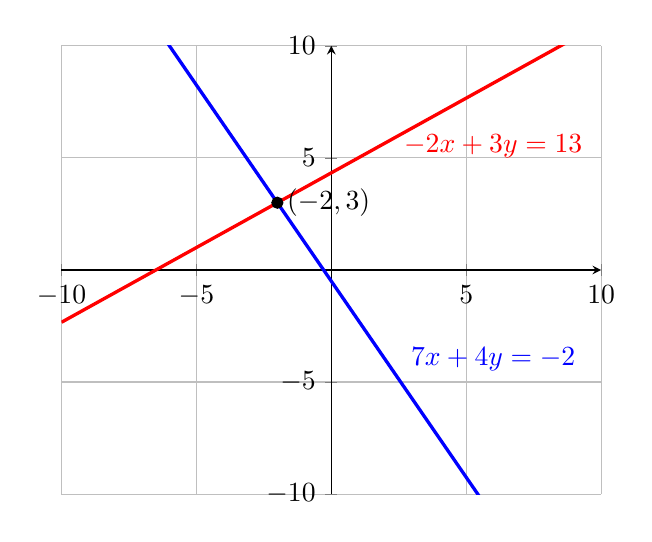
\begin{tikzpicture}
            \begin{axis}[
                axis lines=middle,
                grid=both,
                grid,
                ymin=-10,
                ymax=10,
                xmin=-10, 
                xmax=10
                ]       
                \addplot[mark=none, blue, very thick] coordinates {(-10,17) (10,-18)} node[above] at (axis cs:6,-5) {$7x+4y=-2$};
                \addplot[mark=none, red, very thick] coordinates {(-10,-2.3333) (10,11)} node[below] at (axis cs:6,6.5) {$-2x+3y=13$};
                \addplot[mark=*] coordinates {(-2,3)} node[right] at (axis cs:-2,3) {$(-2,3)$};
            \end{axis}
        \end{tikzpicture}
    \end{center}

    这种可视化方法也适用于三个方程和三个未知数的方程组,但这需要在三维空间中绘制图线。这在实践中可能很难做到,但在技术上是可行的。同样的概念也适用于多个方程和多个未知数,但在四维或更高维上画“线”对我们人类来说是可能是无法想象的!
\end{method}

\begin{method}{多于两个变量:消元!}
    该方法的下一部分建立在第一部分的基础上,通过不断应用第一部分的方法,将两个以上方程(和未知数)的方程组简化为更小的方程组,最终得到两个方程和两个未知数的方程组。我们通过一个三个方程和三个未知数的方程组来说明该方法,如下所示:
    $$
    \begin{cases}
        \enspace\: 6x - 3y + \enspace z = -1 \\
        -3x + 4y - 2z = 12 \\
        \enspace\: 5x + \enspace y + 8z = 6
    \end{cases}
    $$
    第一个目标是消除三个变量中的一个。本质上,这可以通过两种方式之一来完成,就像两个方程和两个未知数的方法一样。假设我们要从方程组中消除 $z$;我们可以尝试以某种方式用 $x$ 和 $y$ 来表示 $z$ 并代入,或者我们可以将某些方程乘以系数并相加,从而消除 $z$。这里唯一的区别是,无论我们选择哪种方法,我们都需要执行两次。我们用第一个方程得到
    \[z = -6x + 3y - 1\]
    将 $z$ 的表达式代入第二个和第三个方程后,我们将得到一个由两个方程和两个未知数组成的方程组。

    思考这个问题的一种方法是,我们需要来自所有三个方程的信息才能最终得出答案,因此在将方程组简化为两个方程时,我们需要以某种方式保留来自所有三个原始方程的信息。$z$ 的表达式来自第一个方程,因此我们需要将其代入其他两个方程以保留我们需要的所有信息。

    将其与以下步骤序列进行比较:整理第一个方程以分离 $z$ 并将其代入第二个方程,然后整理第二个方程式以分离 $z$,将其代入第一个方程。会发生什么?直觉告诉我们,在某种程度上“丢失”了第三个方程的信息,没错,我们将获得一个由两个方程和两个未知数组成的方程组,但它没有足够的信息得到 $x$ 和 $y$ 的唯一解。如果你真的执行了我们刚才描述的步骤(试着这样做来检查我们的工作),化简到最简后,可以得到以下两个方程的“方程组”:
    $$
    \begin{cases}
        9x - 2y = 10 \\
        \frac{9}{2}x - \:y = 5
    \end{cases}
    $$
    这两个方程其实是同一个方程!因此,我们实际上无法求解 $x$ 和 $y$ 的唯一值。

    让我们回到原来的位置,将上面 $z$ 的表达式代入第二和第三个方程
    \begin{align*}
        -3x + 4y - 2 \cdot (-6x + 3y - 1) &= 12 \\
        5x + y + 8 \cdot (-6x + 3y - 1) &= 6
    \end{align*}
    然后化简
    \begin{align*}
        9x - 2y &= 10 \\
        -43x + 25y &= 14
    \end{align*}
    应用第一个问题中的方法之一将解出 $(x, y) = (2, 4)$。有了这两个值,我们就可以代入三个原始方程中的任意一个并求出 $z$;更好的做法是,我们可以使用从第一个方程中得到的 $z$ 的表达式:
    \[z = -6x + 3y - 1 = -6 \cdot (2) + 3 \cdot 4 = 1 = -12 + 12 - 1 = -1\]
\end{method}

\begin{method}{多于两个变量:另一种消元方法!}
    将方程组从三个方程简化为两个方程的另一种方法与前面的“乘加”法有关。使用上面具有三个方程的方程组,我们可能会注意到,第一个方程乘以 $8$,第二个方程乘以 $4$ 后,所有三个方程中 $z$ 的系数都是 $\pm 8$。这使我们能够以简便的方式对方程进行加/减,将方程组简化为两个方程和两个未知数。具体来说,让我们做一遍刚才提到的操作
    \begin{align*}
        48x - 24y + 8z &= -8 \\
        -12x + 16y - 8z &= 48 \\
        5x + y + 8z &= 6
    \end{align*}
    然后将第一个方程与第二个方程相加
    \begin{align*}
        (48x - 12x) + (-24y + 16y) + (8z - 8z) &= -8 + 48 \\
        36x - 8y &= 40
    \end{align*}
    接着将第二个方程与第三个方程相加
    \begin{align*}
        (-12x + 5x) + (16y + y) + (-8z + 8z) &= 48 + 6 \\
        -7x + 17y &= 54
    \end{align*}
    上面操作将产生了两个仅包含 $x$和 $y$ 的方程;此外,我们结合了所有三个原始方程的信息来生成这些方程,所以我们可以确信我们没有“丢失”任何东西。用我们之前讨论的任意一种方法解此新方程组
    $$
    \begin{cases}
        \: 36x - \enspace 8y = 40 \\
        -7x + 17y = 54  
    \end{cases}
    $$
    都会解得 $(x, y) = (2, 4)$。将 $x$ 和 $y$ 的值代入三个原始方程中的任意一个并求出 $z$,即可得到我们要求的最终答案。

    我们也可以执行类似的步骤,从方程组中消除 $y$;例如,我们可以将第一个方程乘以 $4$ 与第二个方程乘以 $3$ 相加,然后用第二个方程减去第三个方程乘以 $4$。这些方法中的任何一种都会得到相同的最终答案,只是其中一些可能会缩短算术步骤或带来“更好计算”的数字(即更少的分数,更小的乘法,等等)。求解具有更多方程的方程组的一般过程:将方程相乘并相加,从方程组中消除一个变量,然后继续这样做,直到只有两个方程和两个未知数;然后,求解这两个变量的值,并反向代入运算,用这些值来求解已消除变量的值。
\end{method}

\subsubsection*{代数练习}

\begin{problem}
    求解关于 $(x, y, z)$ 的以下方程组:

    $$
    \begin{cases}
        \enspace x+y+z=15\\
        2x-y+z=8\\
        x-2y-z=-2
    \end{cases}
    $$

    求解关于 $(x, y, z)$ 的类似方程组:

    $$
    \begin{cases}
        \enspace x+y+z=15\\
        2x-y+z=9\\
        x-2y-z=-2
    \end{cases}
    $$

    比较两个方程组之间 $x$、$y$ 和 $z$ 值的变化。

    哪个变量变化最大?哪个最少?这些变化的比例是多少?

    通过改变方程组第二个方程右侧的常数,你可以使这个比率变多大/多小?
\end{problem}

\begin{problem}
    父亲、母亲和儿子坐在餐厅里吃饭,这时另一个由父亲、母亲和儿子组成的家庭走过来。第二个家庭惊讶于他们与第一个家庭如此相似,于是就问第一个家庭:“你们三个多大了?我猜我们的年龄都差不多”。第一个家庭的父亲恰好是一位数学家,不愿意轻易泄露家人的年龄,于是用一种巧妙的方式“透露”给其他人。他说:“我们现在的年龄加起来是 $72$ 岁,而我恰好是我儿子的六倍。然而,将来当我只是他年龄的两倍时,我们的年龄加起来将是我们现在年龄加起来的两倍。你猜我们多少岁?”\\
    三个家庭成员的年龄有多大?
\end{problem}

\subsection{多项式}

有时我们需要使用平方、立方或更高次幂的变量。一般来说,多项式是我们用于表示一个函数的术语,该函数具有一个或多个整数次幂的变量,乘以系数,然后相加。以下是多项式的一些例子:
\[x^2 - 7x + 1,\quad 7p^6 + 5p^4 + 3p^2 + 2p,\quad \frac{1}{2}z^2 + 9y^2z - 2y + z^3y^2 - 7z\]

这些类型的函数在数学中非常常见和流行,部分原因是它们具有方便的属性,另一部分原因是它们在自然界中的普遍存在。我们将在本书中频繁地看到它们。不过,现在让我们将目光聚焦在只有一个\textit{输入变量}的多项式。

\subsubsection*{多项式的根}

有时,我们会在谜题中定义一个多项式函数,并想知道输入变量是否有任何值可以使输出值为 0。这些让输出值为 0 的输入值称为多项式的\textbf{根}。

识别多项式根的一种方法是将其隐式\textbf{因式分解}为线性项;也就是说,我们尝试将函数表示为一系列乘法而不是加法,因为我们可以声明(至少)其中一个因子为 0 输出值才 0。该技术背后的动机依赖于以下事实:

\begin{quote}
    \textbf{事实:}如果 $a$ 和 $b$ 为实数且 $ab=0$,则 $a=0$ 或 $b=0$(或者两者都等于零)。
\end{quote}

\begin{example}
    我们来看一个具体的例子。尝试分解以下多项式:
    \[p(x) = x^2 + 6x + 8\]
    (将多项式定义为 $p(x)$ 是常见的表示法,其中 $p$ 代表多项式,$x$ 是输入变量,$p(x)$ 是与输入值 $x$ 对应的输出值。)

    你可能已经注意到
    \[p(x) = x^2 + 6x + 8 = (x + 4) \cdot (x + 2) = (x + 4)(x + 2)\]
    (当存在用括号分隔的因子时,删除 $\cdot$ 也是相当常见的,因此我们从现在开始也将采用该约定。)

    这种因式分解之所以有效,是因为我们多次相反地应用分配律。如果我们展开刚刚的因式分解,明确显示其中每一步,它看起来像:

    \begin{align*}
        p(x) &= (x + 4)(x + 2) \\
        &= x(x + 2) + 4(x + 2) \\
        &= (x^2 + 2x) + (4x + 8) \\
        &= x^2 + 2x + 4x + 8 = x^2 + 6x + 8
    \end{align*}

    我们真正写下因式分解步骤是为了注意到项 $+4$ 和 $+2$ 具有乘积 $+8$,这正是常数项,并且它们之和为 $+6$,而这正是 $x$ 项的系数。知道这些因式的后续展开如何进行,我们就可以在不进行检验的情况下写下因式分解。
\end{example}

\subsubsection*{二次因式分解}

让我们以上面示例为例,尝试推广到任何二次函数。如果我们想分解一个二次多项式
\[p(x) = x^2 + bx + c\]
我们要求 $r$ 和 $s$ 的值,使得 $r \cdot s = c$ 且 $r + s = b$。通常,我们可以“通过试算”来做到这一点,或者只需盯着这两个方程思考一分钟即可得出适当的值。(这就是我们在前一个例子中所做的!)

如果 $x^2$ 项的系数不是 $1$ 而是其他数字 $a$,该怎么办?请注意,如果我们可以对多项式 $\frac{p(x)}{a} = x^2+\frac(b)(a)x+\frac{c}{a}$ 进行因式分解,那么我们也可以通过乘以 $a$ 来找到原始多项式 $p(x)$ 的因式分解。这不会影响我们求多项式根(我们最初的目标)的能力,因为我们假设 $a \ne 0$(否则我们一开始就没有二次多项式,也就无需分解它)。一旦我们找到了这个因式分解,就很容易确定 $p(x)$ 的根;因为我们想知道何时 $p(x) = 0$,所以我们可以使用因式分解和上面提到的事实来得出结论:
\begin{align*}
    0 = p(x) = (x + r)(x + s) & \quad \text{ 意味着 } x + r = 0 \text{ 或 } x + s = 0 \\
    & \quad \text{ 即 } x = -r \text{ 或 } x = -s
\end{align*}
也就是说,根为 $-r$ 和 $-s$。

如果我们有一个 $p(x) = x^2 - a^2$ 形式的多项式怎么办?这种特殊类型的函数称为\textbf{平方差},具有快速分解技巧。这是一个二次多项式,因此,按照上面的方法,我们要求 $r,s$ 的值,使得 $rs = -a^2$ 且 $r + s = 0$(因为 $p(x)$ 中没有 $x$ 项)。第二个条件告诉我们 $r = -s$,代入第一个条件可得 $r^2 = a^2$。 因此,令 $r = a$ 和 $s = -a$ 实现因式分解 $p(x) = (x - a)(x + a)$,因此根为 $\pm a$。(请注意,$r = -a$ 和 $s = a$ 也满足这两个条件,但实际上会产生相同的 $p(x)$ 因式分解。)

类似的技巧有时可以应用于更高\textbf{次}的多项式(回想一下,“次”意味着输入变量的最高次幂)。例如,以下多项式的次数为 4
\[p(x) = 4x^4 - x^2 - 3\]
如果我们定义 $y = x^2$ 并将其写成二次多项式,我们就可以轻松分解它
\[p(y) = 4y^2 - y - 3 = (4y + 3)(y - 1)\]
请注意,你可以考虑 $y^2$、$y$ 的系数和常数项的分解,从而直接跳转到我们上面的分解方法或除法技巧。这里,我们想要分解 $\frac{p(y)}{4} = y^2-\frac{1}{4}=\frac{3}{4}$,因此我们令 $rs = -\frac{3}{4}$ 和 $r + s =-\frac{1}{4}$;$r=-1, s=+\frac{3}{4}$ 满足,所以我们得到因式分解
\[\frac{p(x)}{4} = (y+(-1))\Big(y+\frac{3}{4}\Big)\]
化简得
\[p(x) = 4(y-1)\Big(y+\frac{3}{4}\Big) = (y-1)(4y+3)\]
这正是我们之前的方法。

\subsubsection*{一根一因子}

当然,这种识别根的技巧也可以反向发挥作用:如果我们可以轻松地找到多项式的根,这可以帮助我们识别其中一个因子。举个例子,请看下面的三次多项式,看看能否“通过试算”找到根;也就是说,看看能否找到 $x$ 的输入值,使 $p(x)$ 的计算结果为零:
\[p(x) = x^3 - 3x + 2\]
如果您还没有找到,你可以试着代入一些“简单值”,例如前几个整数(正数和负数),看看会发生什么。如果这样做,你会发现 $p(1) = 1 - 3 + 2 = 0$。因此,我们知道多项式 $p$ 的因式分解应包含因子 $(x - 1)$,因为它对应于根 $x = 1$。知道了这一点,我们就可以将 $p(x)$ 除以因子 $(x - 1)$,从而可以进一步对商进行因式分解并确定 $p$ 的所有根。

\subsubsection*{多项式“除法”}

那么我们要如何除多项式呢?我们要求另一个多项式 $q(x)$ 使得 $p(x) = q(x) \cdot (x - 1)$,或者换句话说,我们需要找到 $\frac{p(x)}{x-1}$。找到此类函数的一种方法是使用与你在中学学习整数除法时学到的\textbf{长除法}原理。相同的概念也适用于多项式函数!回想一下除法的工作原理,并尝试通过一些基本示例 --- 例如 $22 \div 7$ --- 来唤起你对除法工作原理的记忆。

现在,让我们尝试将同样的原理应用于多项式。这是将长除法的思想应用于 $\frac{x^3-3x+2}{x-1}$ 的示例:

\[
\arraycolsep=1pt
\begin{array}{*1r @{\hskip\arraycolsep}c@{\hskip\arraycolsep} *{9}r}
        &          &   &      &   & x^2 & + &  x & - & 2 &  \\
\cline{2-11}
x-1     & \longdiv &   & x^3  &   &  & -    & 3x & + & 2 &  \\
        &          & - & x^3  & + & x^2 &   &    &   &   &  \\
\cline{3-6}
        &          &   &      &   & x^2 & - & 3x &   &   &  \\
        &          &   &      & - & x^2 & + &  x &   &   &  \\
\cline{5-8}
        &          &   &      &   &     & - & 2x & + & 2 &  \\
        &          &   &      &   &     &   & 2x & - & 2 &  \\
\cline{7-11}
        &          &   &      &   &     &   &    &   & 0 &  \\
\end{array}
\]

在该方法的每次迭代中,我们尝试找到可以“得到”更高次幂的最大“因子”。在这种情况下,这些因子只是乘以 $x$ 的幂;我们确定可以“得到”当前相关项的 $x$ 的最大幂。由于被除数为 $x^3$,除数为 $x$,因此我们在除法线上方写上 $x^2$。然后,我们将 $(x-1)$ 乘以 $x^2$,将其写在被除数下方,然后相减求出余数。

重复相同的过程,直到除法线上方出现常数项(即 $x^0$ 的倍数)并查看余数。由于这里的余数为 $0$,所以我们知道我们得到了一个没有余数的因式分解。然后,我们注意到 $r=2, s=-1$ 满足 $r+s=1$ 且 $rs=-2$,因此结果二次多项式可以进一步分解,最终得到
\[p(x) = (x - 1)(x - 1)(x + 2) = (x - 1)^2(x + 2)\]

多项式的次数为 $3$,但函数只有 $2$ 个根。这是否让你感到奇怪?你能想到一个只有 $1$ 个根的 $3$ 次多项式吗?没有根的 $3$ 次多项式会是怎样?拥有 $4$ 个根、$5$ 个根或更多根呢?这有可能吗?为什么可能或为什么不可能?如果是 $4$ 次多项式会怎样?$n$ 次呢?你能确定多项式根的数量与其次数的关系吗?

\subsubsection*{因式展开}

有时,在解决难题时,我们会从多项式的因式分解开始,并希望完全扩展因子,以便我们可以确定特定项的系数。我们如何快速、轻松地将多项式相乘?本质上,我们一遍又一遍地应用分配律,而不必写出所有步骤(尽管这种基本的、一步一步的程序保证有效,所以如果你不确定你的答案是否正确,最好回去彻底检查每一步)。

有种特殊的情况可以减少所涉及的步骤,那就是当我们需要展开像 $(a+b)^n$ (其中 $a$ 和 $b$ 代表任意常量或变量,$n$ 为整数)这样的因式分解时。在这种特定情况下,有一种方便的方法来确定展开多项式的系数,这些值来自\textbf{帕斯卡三角}。

这是一种将整数行排列成三角形的排列,其中每行对应于这种展开中 $n$ 的特定值。生成帕斯卡三角形的诀窍是先将前两行全写为 $1$,再将三角形的外侧“边”全写为 $1$。在三角形的内部,任何条目都可以通过将该条目左上方和右上方的两个条目相加得到。试着自己生成三角的前几行,并与下面的三角进行比较,以确保你正确完成了该过程。

\begin{center}
    \begin{tabular}{rccccccccc}
        $n=0$: &    &    &    &    &  1\\\noalign{\smallskip\smallskip}
        $n=1$: &    &    &    &  1 &    &  1\\\noalign{\smallskip\smallskip}
        $n=2$: &    &    &  1 &    &  2 &    &  1\\\noalign{\smallskip\smallskip}
        $n=3$: &    &  1 &    &  3 &    &  3 &    &  1\\\noalign{\smallskip\smallskip}
        $n=4$: &  1 &    &  4 &    &  6 &    &  4 &    &  1\\\noalign{\smallskip\smallskip}
    \end{tabular}
\end{center}

我们将 $n$ 值写在左侧,表示与展开 $(a+b)^n$ 的对应关系。一般来说,展开式的任何项都是某个系数(取自帕斯卡三角)乘以 $a^kb^{n-k}$,其中 $k$ 的值介于 $0$ 到 $n$ 之间。也就是说,展开式每一项种,$a$ 和 $b$ 的幂之和必须为 $n$。三角形任何一行中的数字都是按照 $a$ 的幂降序书写的,所以第一个 $1$ 是 $a^n$ 的系数,下一个数字是 $a^{n-1}b$ 的系数,依此类推。

如果我们要展开 $(a + b)^2$,我们会读取帕斯卡三角的 $n = 2$ 行,得到系数为 $1, 2, 1$,这些系数分别是 $a^2, ab, b^2$ 的系数。因此,
\[(a + b)^2 = a^2 + 2ab + b^2\]
我们也可以轻松地手动完成展开。但如果我们要展开 $(x^2+2)^4$ 怎么办?这不是手动能快速完成的,所以让我们试试使用帕斯卡三角会发生什么。$n = 4$ 行告诉我们 $a^4, a^3b, a^2b^2, ab^3, b^4$ 的系数分别为 $1, 4, 6, 4, 1$,其中 $a = x^2, b = 2$。因此,我们可以写成
\begin{align*}
    (x^2+2)^4 &=  1 \cdot (x^2)^4 + 4 \cdot (x^2)^3 \cdot 2 + 6 \cdot (x^2)^2 \cdot (2)^2 + 4 \cdot x^2 \cdot (2)^3 + 1 \cdot (2)^4 \\
    &=  x^8 + 4 \cdot x^6 \cdot 2 + 6 \cdot x^4 \cdot 4 + 4 \cdot x^2 \cdot 8 + 16 \\
    &= x^8 + 8x^6 + 24x^4 + 32x^2 + 16
\end{align*}
尝试逐步执行此展开并进行比较。实际上,帕斯卡三角有一些非常有趣的性质,这些性质深深植根于其他一些数学概念中,这些性质在\textbf{组合数学}领域特别有用。事实上,我们稍后将更详细地研究其中许多性质!例如,你可能想知道为什么这个过程 --- 添加上面的两个条目 --- 会生成与这样的展开因子相对应的条目。当我们讨论\textbf{二项式定理}及其相关思想时,我们将证明它的有效性!(如果您感到好奇,请参阅 \ref{sec:section8.4.4} 节。)

\subsubsection*{配方}

在得出重要结果之前,我们还需要提及一个与多项式相关的技巧。有时,将多项式重写为平方项加常数项是非常有用的,这样我们就可以以方便的方式分离变量和常数。这相当于添加再减去一个特定项,因此,总的来说,我们在多项式中添加了 $0$,但选择该项的方式可以让我们方便地重写多项式的项。这个过程被称为\textbf{配方},即我们添加一项来创建平方因子,并通过减去相应的量来保持多项式不变。

让我们通过一个例子来说明这个过程,然后再尝试进行概括。请看下面的多项式:
\[p(x) = x^2 + 8x + 9\]
因式分解在这里并不明显,所以让我们尝试配方。我们想要得到类似 $(x + a)^2$ 这样的项,其中我们知道 $x$ 的系数为 $1$,因为多项式种有 $1 \cdot x^2$。将其展开得 $x^2+2ax+a^2$。由于我们需要得到 $8x$,所以我们应该令 $a = 4$。因此展开得到 $x^2 + 8x + 16$,但原式的常数项为 $+9$,所以我们向原多项式中加上 $7$ 再减去 $7$:
\[p(x) = x^2 + 8x + 9 + 7 - 7 = (x^2 + 8x + 16) - 7 = (x + 4)^2 - 7\]
上面的式子看起来眼熟吗?准确地说,它是平方差,我们知道如何分解它:
\begin{align*}
    p(x) &= x^2 + 8x + 9 = (x + 4)^2 - 7 = (x + 4)^2 - \Big(\sqrt 7\Big)^2 \\
    &= \Big(x+4+\sqrt 7\Big)\Big(x+4-\sqrt 7\Big)
\end{align*}
因此,该多项式的根为 $x=-4-\sqrt 7$ 和 $x=-4+\sqrt 7$。

让我们来泛化一下!假设我们从以下形式的二次多项式开始
\[p(x) = ax^2 + bx + c\]
为了能够配方,我们需要添加再减去一个特定项。我们之前是如何找到这个项的?像 $(rx + s)^2$ 这样的项展开后得 $r^2x^2 + 2rsx + s^2$,并且为了将这些系数与原多项式的系数相匹配,我们发现需要让 $r^2 = a$,所以我们需要令 $r = \sqrt{a}$。(注意,这里要求 $a \ge 0$!如果 $a<0$ 该怎么办?)然后,为了让 $2rs = b$,我们需要令 $s = \frac{b}{2r} = \frac{b}{2\sqrt{a}}$,接着,当它展开时,我们添加 $s^2 = \frac{b^2}{4a}$,再从多项式中减去。

下面公式执行了上述步骤,并进行一些额外的代数整理,让项“更好看”:
\begin{align*}
    p(x) &= ax^2 + bx + c = ax^2 + bx + \frac{b^2}{4a} + c - \frac{b^2}{4a}\\
    &=\Big(\sqrt{a}x+\frac{b}{2\sqrt{a}}\Big)^2+\Big(c- \frac{b^2}{4a}\Big)\\
    &=\Big(\sqrt{a}\Big(x+\frac{b}{2a}\Big)\Big)^2+\Big(c- \frac{b^2}{4a}\Big)\\
    &=a\Big(x+\frac{b}{2a}\Big)^2+\Big(c- \frac{b^2}{4a}\Big)
\end{align*}
现在,我们知道了如何对给定的任何二次多项式进行配方!

\subsubsection*{可视化配方}

有一个记住如何执行上述配方过程的有效方法。它基于正方形和矩形面积的可视化表示。

假设 $a, b>0$,这样我们就可以从几何角度将 $ax^2+bx$ 解释为矩形的面积。具体来说,我们将 $ax^2$ 项视为正方形的面积。这意味着正方形的边长为 $\sqrt{a} \cdot x$: 

\begin{center}
    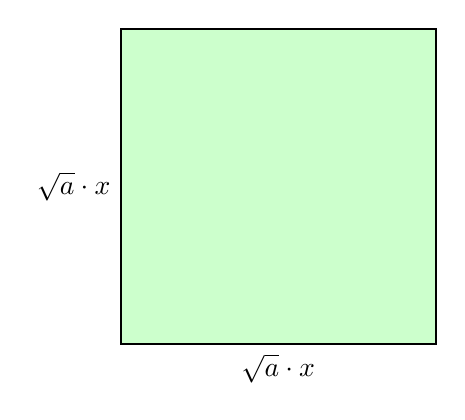
\begin{tikzpicture}[thick, scale=1]
        \fill [color=green,opacity=0.2] (0,0) rectangle +(4,4);
        \draw (0,0) rectangle +(4,4);
        \path (0,0) -- (4,0) node[midway,below] {$\sqrt{a}\cdot x$};
        \path (0,0) -- (0,4) node[midway,left] {$\sqrt{a}\cdot x$};
    \end{tikzpicture}
\end{center}

那么我们应该如何表示 $bx$ 这一项呢?我们要把正方形扩展到更大的正方形;这就是配方的意义。因此,我们需要围绕正方形构建一些矩形,这将有助于我们实现这一目标。让我们将 $bx$ 项代表的面积分成两个矩形,每个矩形的面积为 $\frac{b}{2}x$。由于矩形必须有一条边的长度为 $\sqrt{a} \cdot x$,并且我们希望矩形面积为 $\frac{b}{2}x$,因此另一条边长必然为 $\frac{b}{2\sqrt{a}}$: 

\begin{center}
    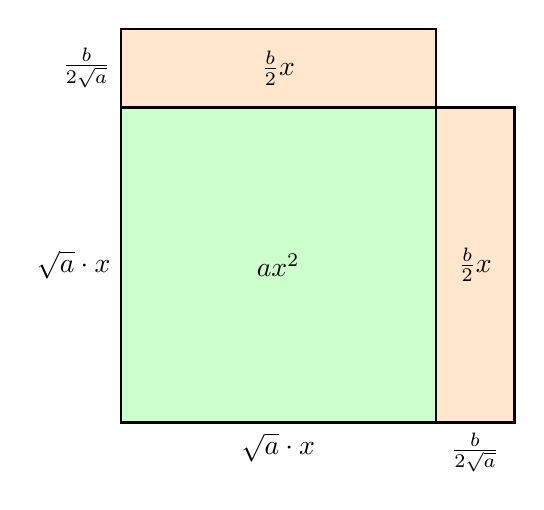
\begin{tikzpicture}[thick, scale=1]
        \fill [color=green,opacity=0.2] (0,0) rectangle +(4,4);
        \draw (0,0) rectangle +(4,4) node[pos=.5, align=center]{$ax^2$};
        \path (0,0) -- (4,0) node[midway,below] {$\sqrt{a}\cdot x$};
        \path (0,0) -- (0,4) node[midway,left] {$\sqrt{a}\cdot x$};

        \fill [color=orange,opacity=0.2] (4,0) rectangle +(1,4);
        \draw (4,0) rectangle +(1,4) node[pos=.5, align=center]{$\frac{b}{2}x$};
        \path (4,0) -- (5,0) node[midway,below] {$\frac{b}{2\sqrt{a}}$};

        \fill [color=orange,opacity=0.2] (0,4) rectangle +(4,1);
        \draw (0,4) rectangle +(4,1) node[pos=.5, align=center]{$\frac{b}{2}x$};
        \path (0,4) -- (0,5) node[midway,left] {$\frac{b}{2\sqrt{a}}$};
    \end{tikzpicture}
\end{center}

我们需要添加什么才能使上面的图形变成为一个正方形?我们发现只需在右上角填充一个小正方形即可。小正方形边长为 $\frac{b}{2\sqrt{a}}$,因此它的面积 --- 我们需要添加的项--- 为 $\frac{b^2}{4a}$。

\begin{center}
    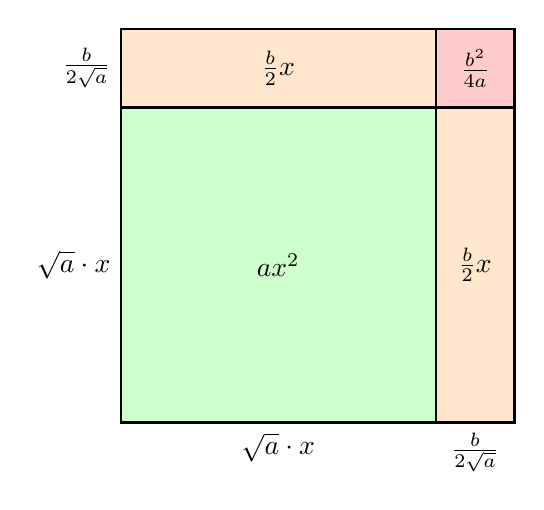
\begin{tikzpicture}[thick, scale=1]
        \fill [color=green,opacity=0.2] (0,0) rectangle +(4,4);
        \draw (0,0) rectangle +(4,4) node[pos=.5, align=center]{$ax^2$};
        \path (0,0) -- (4,0) node[midway,below] {$\sqrt{a}\cdot x$};
        \path (0,0) -- (0,4) node[midway,left] {$\sqrt{a}\cdot x$};

        \fill [color=orange,opacity=0.2] (4,0) rectangle +(1,4);
        \draw (4,0) rectangle +(1,4) node[pos=.5, align=center]{$\frac{b}{2}x$};
        \path (4,0) -- (5,0) node[midway,below] {$\frac{b}{2\sqrt{a}}$};

        \fill [color=orange,opacity=0.2] (0,4) rectangle +(4,1);
        \draw (0,4) rectangle +(4,1) node[pos=.5, align=center]{$\frac{b}{2}x$};
        \path (0,4) -- (0,5) node[midway,left] {$\frac{b}{2\sqrt{a}}$};

        \fill [color=red,opacity=0.2] (4,4) rectangle +(1,1);
        \draw (4,4) rectangle +(1,1) node[pos=.5, align=center]{$\frac{b^2}{4a}$};
    \end{tikzpicture}
\end{center}

看呐!这与我们上面通过代数推导得出的项完全相同。通过添加它,我们可以将这些项分解为完全平方。只需要再将其也减去,以确保原表达式不变。

这是一个需要记住的有用技巧。它可以提醒你配方的过程动机以及如何实现它。不过,你应该思考一件事:为什么这种可视化表示有效?我们必须假设 $a, b > 0$ 才能画出这些图,那么为什么无论 $a$ 和 $b$ 是什么,通向公式都有效呢?

\subsubsection*{二次函数求根公式}

让我们回到求多项式的根的问题。具体来说,让我们回忆一下\textbf{二次函数求根公式}。你可能已经记住这个公式是“求解二次方程”的一种方法,但你知道它为什么有效吗?让我们试着弄清楚吧!一般来说,我们从以下形式的二次多项式开始
\[p(x) = ax^2 + bx + c\]
其中 $a \ne 0$(否则,它就不是二次多项式),并且我们想要求 $p(x) = 0$ 时 $x$ 的值。(你是否尝试过回答我们上面提出的关于此类多项式有几个根的问题?在以下推导过程中请记住这些概念。)将该多项式因式分解为线性因子很麻烦,所以我们使用上面介绍的方法:配方。该方法的好处是,我们可以设置 $p(x)=0$,并在配方后重新整理项来求解 $x$。观察:
\[0 = p(x) = ax^2 + bx + c =a\Big(x+\frac{b}{2a}\Big)^2+\Big(c- \frac{b^2}{4a}\Big)\]
化简可得
\[\frac{b^2}{4a} -c = a\Big(x+\frac{b}{2a}\Big)^2\]

现在,我们要开始“撤消”此处的配方来求解 $x$,这需要对两边求平方根。但如果 $\frac{b^2}{4a} -c < 0$ 呢?我们根本无法求平方根!如果 $\frac{b^2}{4a} -c = 0$ 呢?会有问题吗?当 $\frac{b^2}{4a} -c > 0$ 时会有什么问题吗?这些问题与我们之前关于多项式可能有的根数相关。你可能已经(正确地)推断出二次多项式最多可以有两个根,但在这里我们发现二次多项式可能有一个或零个根(及其原因)!

\begin{itemize}
    \item 当 $\frac{b^2}{4a} -c < 0$ 时,那么 $x$ 的任何值都\textit{不}可能满足上面推导中的最后一行公式。因此,$p(x)$ 无实数根。
    \item 当 $\frac{b^2}{4a} -c = 0$ 时,那么对上面最后一行公式两边取平方根是完全有效的,但只会产生\textit{唯一一个 }$x$ 值:
    \begin{align*}
        \frac{b^2}{4a} -c = 0 &= a\Big(x+\frac{b}{2a}\Big)^2 \\
        0 &= x+\frac{b}{2a} \\
        x &= -\frac{b}{2a}
    \end{align*}
    \item 当 $\frac{b^2}{4a} -c > 0$ 时,此时,我们预期 $p(x)$ 有\textit{两个}根,因为两边取平方根会引入两个可能的解。一般来说,当我们遇到像 $s^2 = t$ 这种情况时,我们可以说唯一可能的解是 $s =\sqrt{t}$ 和 $s = -\sqrt{t}$,但我们必须同时考虑两者(通常将其写做 $s = \pm\sqrt{t}$)。在这种情况下求解 $x$ 得
    \begin{align*}
        \frac{b^2}{4a} -c &= a\Big(x+\frac{b}{2a}\Big)^2 \\
        \pm\sqrt{\frac{b^2-4ac}{4a}} &= \sqrt{a}\Big(x+\frac{b}{2a}\Big) = \sqrt{a}x+\frac{b}{2\sqrt{a}} \\
        -\frac{b}{2\sqrt{a}}\pm\frac{\sqrt{b^2-4ac}}{\sqrt{4a}} &= \sqrt{a}x \\
        -\frac{b}{2a}\pm\frac{\sqrt{b^2-4ac}}{\sqrt{4a^2}} &= x
    \end{align*}
    现在,我们必须小心对待之前进行的平方根观察。一般来说,$\sqrt{4a^2} = \pm2a$,但我们知道分子上的平方根项已经有一个相关的 $\pm1$ 因子,因此分母上的因子不会改变这一点。因此,我们可以得出结论
    \[x = -\frac{b}{2a}\pm\frac{\sqrt{b^2-4ac}}{2a} = \frac{-b\pm\sqrt{b^2-4ac}}{2a}\]
    这就是二次函数求根公式!
\end{itemize}

请记住,推导的最后一种情况是在 $\frac{b^2}{4a} -c > 0$ 的假设下进行的。当 $\frac{b^2}{4a} -c = 0$ 时,该公式依然适用吗?在这种假设下,我们是否可以执行与上面相同的步骤?为什么可以或者为什么不可以?

\subsubsection*{问题}

\begin{problem}
    找出 $a$ 的所有可能值,使 $x-a$ 是 $x^2+2ax-3$ 的因子。
\end{problem}
\begin{problem}
    找出 $b$ 的所有可能值,使得 $x^3 + b$ 可以被 $x + b$ 整除,没有余数。
\end{problem}
\begin{problem}
    对于任意自然数 $n$,因子 $x^n - 1$。
\end{problem}
\begin{problem}
    确定如下公式定义的 $x$ 的值
    \[x = \sqrt{2+\sqrt{2+\sqrt{2+\sqrt{2+\dots}}}}\]
    \begin{hint}
        尝试用 $x$ 本身来表示无限嵌套的平方根。
    \end{hint}
\end{problem}
\begin{problem}
    用配方法证明正数 $n$ 及其倒数之和始终大于或等于 $2$,并且唯一使和等于 $2$ 的数字是 $n = 1$。
    \begin{hint}
        求和,加减 $2$,然后重新整理。
    \end{hint}
\end{problem}
\begin{problem}
    如何求 $ax^4 + bx^2 + c$ 形式的四次多项式的根?
\end{problem}

\subsection{集合漫谈}

我们已经提到了一些特定类型的数字,但我们想具体定义我们将来要使用的数字集。这些数字集合都由一个特定字母用黑板粗体表示。\textbf{自然数}(也称为整体数(whole numbers)或计数数(counting numbers))之所以被称为自然数,是因为当我们计数物体时,用自然数感觉很“自然”。自然数可以写做
\[\mathbb{N} = \{1, 2, 3, 4, 5, \dots\}\]
(自然数有一个更具体更技术性的定义,我们将在稍后解释。)\\
我们用 $\mathbb{N}$ 表示 “自然(natural)”

使用 $\mathbb{N}$,我们可以定义一个相关的数字集合:所有\textbf{整数}的集合,它包含了自然数、0和负自然数。整数可以写做
\[\mathbb{Z} = \{\dots, -3, -2, -1, 0, 1, 2, 3, \dots\}\]
字母 $\mathbb{Z}$ 来自德语单词 \textit{Zahlen},意思是“数字”。

从整数集合,我们可以定义\textbf{有理数}的集合。这些数字可以表示为整数的比率,但它们似乎没有像集合 $\mathbb{N}$ 和 $\mathbb{Z}$ 那样自然的“列表”,所以我们不能像上面那样书写这个集合。为此,我们使用一个非常常见的集合表示法,如下所示:
\[\mathbb{Q} = \Big\{\frac{a}{b} \mid a,b \in \mathbb{Z} \text{ 且 } b \ne 0\Big\}\]
读作:
\begin{quote}
    “有理数集是所有 $\frac{a}{b}$ 形式的数的集合,其中 $a$ 和 $b$ 都是整数,且 $b$ 不为零。”
\end{quote}
这表达了有理数是分数的必要信息,其中分子和分母都是整数(但分母不能为 $0$,因为除以 $0$ 是不允许的)。我们使用字母 $\mathbb{Q}$ 表示有理数,是因为 $\mathbb{R}$ 已经被用于表示实数,而 $\mathbb{Q}$ 是上一个可用的字母。此外,$\mathbb{Q}$ 包含所有整数的商,所以这也是有道理的!

\textbf{实数} $\mathbb{R}$ 有一个非常技术性的定义,遗憾的是,我们无法在本书中全面深入研究。(这恰恰表明,从数学上定义这个集合是多么困难!) 目前,思考实数的一种方法是通过\textbf{数轴}。实数是数轴上所有的数字,而 $\mathbb{N}$、$\mathbb{Z}$ 和 $\mathbb{Q}$ 中的数字是数轴上的特定数字,它们并不构成整条数轴。某种程度上,$\mathbb{R}$ 是 $\mathbb{Q}$ 的“补全”,即“填补有理数之间的空白”。

\subsection{符号加油站}\label{sec:section1.3.5}

一种流行且方便的求和与求积的写法是使用缩写符号,将多个项或因子写成一种通用的形式。例如,如果我们想谈论前 500 个自然数之和,该怎么写呢?写出总和的全部 500 项会很乏味,所以 $1+2+3+\dots+499+500$ 是更常见的写法。(事实上,我们已经使用过这样的省略号。 你明白我们的意思吗?)这种写法很流行,并且确实表达了观点,但一些数学家对中间多余的省略号感到不满。我们推迟到现在才讨论这个问题,是因为符号通常很难学习和理解。我们并没有立即用新符号轰炸你,而是诉诸我们对 “$\dots$” 作用的直观理解。

既然我们已经提出来了,让我们看看如何避免使用省略号。为了写出我们上面提到的求和,我们将使用以下符号:
\[1+2+3+\dots+499+500 = \sum_{i=1}^{500}i\]
大写西格玛 $\sum$ 来自对应英文字母 S 的希腊字母,代表“求和”。\textbf{索引} $i$ 告诉我们求和的各个项的值。在 $\sum$ 符号下面写 $i = 1$,在 $\sum$ 符号上面写 $500$ 意味着我们让 $i$ 表示 $1$ 到 $500$(含)之间的所有自然数值。我们将这些值代入求和项的通用表达式,在本例中就是 $i$。因此,根据要求,求和项为 $1,2,3,\dots,500$。通过改变求和项表达式和/或索引的值,试着找到一些其他的写法。如果我们想求前 500 个偶自然数之和怎么办?想求 500 以内(含)所有偶自然数又该怎么办呢?尝试用上面的符号样式写出这些求和。

与此相关的是 $\prod$ 表示法。如果我们想查看前 500 个自然数的乘积,我们将遵循相同的约定来识别索引值和通项:
\[1+2+3+\dots+499+500 = \prod_{i=1}^{500}i\]
大写派 $\prod$ 来自对应英文字母 P 的希腊字母,代表“求积”。再次尝试通过更改求积项和/或索引值以不同的方式表达上面公式。如果我们想求前 500 个偶自然数的乘积怎么办?想求 500 以内(含)所有偶自然数之积又该怎么办呢?尝试用上面的符号样式写出这些求积。

\subsubsection*{问题}

\begin{problem}
    用自然语言来描述以下等式的含义:
    \[\sum_{i=1}^{n}i^2 = \frac{n(n+1)(2n+1)}{6}\]
\end{problem}
\begin{problem}
    用适当的符号表达 $2$ 的前 $n$ 次幂的和与积,从 $2^0=1$ 开始。你能证明这个求和和求积公式吗?
\end{problem}
\begin{problem}
    考虑 $17$ 到 $33$(含)之间的所有奇数之和。索引 $0$ 开始,用求和符号写出这个求和公式。现在试着将索引从 $1$ 开始,重写求和公式。现在试着将索引从 $8$ 开始,重写求和公式,然后将索引从 $9$ 开始。以下哪一个感觉“更自然”?为什么?
\end{problem}


\newpage
% !TeX root = ../../book.tex
\section{智力谜题}


\newpage
% !TeX root = ../../book.tex
\section{学而时习之}


\newpage
% !TeX root = ../../book.tex
\section{展望}

% !TeX root = ../../book.tex
\chapter{数学归纳法}

% !TeX root = ../../book.tex
\section{导论}

\newpage
% !TeX root = ../../book.tex
\section{案例研讨}

\subsection{构建更大的立方体}

为了引出数学归纳法的整体方法,让我们看一道几何题并一起解决它。这个例子是精心挑选出来的,旨在说明当问题具有特定类型的结构时,数学归纳法如何与之关联;具体来说就是,某些真理、事实或洞察\textit{取决于}、\textit{依赖于}或可以从“先前的”事实\textit{推导}得出。这种对先前案例(或多个案例)的依赖使得过程具有\textit{归纳性},当我们观察到这种现象时,应用\textit{归纳法}几乎总是一个好主意。

\subsubsection*{$1$ 阶立方体到 $2$ 阶立方体}

让我们来考察一下立方数,尤其是,让我们试着用前一个立方数来描述一个立方数。想象一个 $1 \times 1 \times 1$ 的立方体,让它作为单位块。我们如何通过添加 $1 \times 1 \times 1$ 的块来构建尺寸为 $2 \times 2 \times 2$ 的“下一个最大”立方体?我们需要添加多少个?从算术上讲,我们知道答案:$2^3 = 8$ 且 $1^3 = 1$,因此我们需要添加 $7$ 个块才能得到正确的体积。好吧,这是一个具体的答案,但它并没有完全告诉我们如何排列这 $7$ 个块来构成一个立方体,也没有让我们深入了解如何回答构建\textit{更大}立方体这个问题。最终,我们想回答的是,需要多少块才能从 $100 \times 100 \times 100$ 的立方体构建出 $101 \times 101 \times 101$ 的立方体,而无需执行大量繁琐的计算;也就是说,我们希望最终找到问题的答案:给定一个 $n \times n \times n$ 的立方体,我们需要添加多少块才能将其构建为 $(n+ 1) \times (n+ 1) \times (n+ 1)$ 的立方体?考虑到这一点,让我们仔细思考这个最初的案例,并尝试用一般性的论点来回答它。

给定一个单位块,并且我们知道必须向其添加 $7$ 个块,让我们试着确定这 $7$ 个块应该放置在哪里,以形成 $2 \times 2 \times 2$ 的立方体。(为了简单起见,对于 $n$ 的任意值,我们把大小为 $n \times n \times n$ 的立方体称为 $n$ 阶立方体。在这个例子中,$n$ 的值只取自然数,即非负整数。)查看下面 $1$ 阶立方体和 $2$ 阶立方体的图片,并试着解释如何从一个立方体构建另一个立方体。

\begin{center}
    \begin{tikzpicture}
        \pic {annotated cuboid};

        \foreach \x in {0,1}
            \foreach \y in {0,1}
                \foreach \z in {0,1}
                    \pic [fill=white] at (4+\x,\y,\z) {annotated cuboid};
        % \pic [very thick,densely dashed,draw=blue] at (5,0) {annotated cuboid={width=30, height=5, depth=10, opacity=0.2}};
    \end{tikzpicture}
\end{center}

这是我们想要使用的一个合理的解释,因为它能指导我们给出从 $n$ 阶立方体构建 $(n+1)$ 阶立方体的一般解释,并且它是一种数学上优雅且简单的解释。从上面的 $1$ 阶立方体开始,将 $3$ 个暴露的面“放大”适当的量,在本例中为 $1$ 块。到目前为止,这占 $7$ 个块中的 $3$ 个:$2^3 = 1^3+3+\underline{\qquad}$。现在还缺哪里?

\begin{center}
    \begin{tikzpicture}
        \pic {annotated cuboid};
        \pic at (1,-1,0) {annotated cuboid};
        \pic at (0,-1,1) {annotated cuboid};
    \end{tikzpicture}
\end{center}

我们刚刚添加的块在每对块之间都产生了“间隙”,并且每个“间隙”都可以用一个块填充。这占了 $7$ 个块中的 $3$ 个:$2^3 = 1^3+3+3+\underline{\qquad}$。接下来呢?

\begin{center}
    \begin{tikzpicture}
        \pic {annotated cuboid};
        \foreach \x in {0,1}
            \foreach \y in {0,1}
                    \pic [fill=white] at (\x,\y,0) {annotated cuboid};
        \pic [fill=white] at (0,0,1) {annotated cuboid};
        \pic [fill=white] at (0,1,1) {annotated cuboid};
        \pic [fill=white] at (1,0,1) {annotated cuboid};
        % \pic [very thick,densely dashed,draw=blue] at (5,0) {annotated cuboid={width=30, height=5, depth=10, opacity=0.2}};
    \end{tikzpicture}
\end{center}

只剩下一个块需要填充,位于最顶角。添加这个块就完成了 $2$ 阶立方体的构建,并且我们还得到了如何使用以下图形和方程以数学的方式描述我们的构建过程:

\begin{center}
    \begin{tikzpicture}
        \pic {annotated cuboid};

        \pic [densely dashed] at (3, 0) {annotated cuboid};
        \pic [very thick,draw=blue] at (4.2,0,0) {annotated cuboid};
        \pic [very thick,draw=blue] at (3,1.2,0) {annotated cuboid};
        \pic [very thick,draw=blue] at (3,0,1.4) {annotated cuboid};

        \pic [densely dashed] at (7.5,1,0) {annotated cuboid};
        \pic [densely dashed] at (8.5,0,0) {annotated cuboid};
        \pic [densely dashed] at (7.5,0,1) {annotated cuboid};
        \pic [very thick,draw=red] at (8.7,1.2,-0.1) {annotated cuboid};
        \pic [very thick,draw=red] at (7.3,1,1.4) {annotated cuboid};
        \pic [very thick,draw=red] at (8.7,-0.2,1) {annotated cuboid};

        \foreach \x in {0,1}
            \foreach \y in {0,1}
                \pic [densely dashed, fill=white] at (12+\x,\y,0) {annotated cuboid};
        \pic [densely dashed, fill=white] at (12,0,1) {annotated cuboid};
        \pic [densely dashed, fill=white] at (12,1,1) {annotated cuboid};
        \pic [densely dashed, fill=white] at (13,0,1) {annotated cuboid};
        \pic [very thick,draw=olivegreen] at (13.3,1,1.4) {annotated cuboid};
    \end{tikzpicture}
\end{center}

\begin{center}
    \large $2^3 = 1^3+\textcolor{blue}{3}+\textcolor{red}{3}+\textcolor{olivegreen}{1}$
\end{center}

\subsubsection*{$2$ 阶立方体到 $3$ 阶立方体}

现在我们可能对如何描述这个过程有了更好的了解,但让我们多考察两个案例,以确保我们有完整的想法。

让我们从 $2$ 阶立方体开始,构造一个 $3$ 阶立方体。(如果碰巧你手上有各种尺寸的魔方,你甚至可以手动尝试一下!)我们可以遵循与上一个案例类似的步骤,只需适当更改数字即可。从相似的图形开始

\begin{center}
    \begin{tikzpicture}[scale=1]
        \pic {annotated cuboid};
        \foreach \x in {0,1}
            \foreach \y in {0,1}
                \foreach \z in {0,1}
                    \pic [fill=white] at (\x,\y,\z) {annotated cuboid};
        \foreach \x in {0,1,2}
            \foreach \y in {0,1,2}
                \foreach \z in {0,1,2}
                    \pic [fill=white] at (\x+4,\y,\z) {annotated cuboid};
    \end{tikzpicture}
\end{center}

可见我们需要“放大” $2$ 阶立方体的三个暴露面,但在这种情况下,我们需要放大的量与以前($1$ 阶立方体)\textit{不同},因为我们现在使用的是更大的初始立方体。具体来说,每个面必须放大 $2 \times 2$ 的\textit{正方形}块(而在之前的情况下,我们添加了 $1 \times 1$ 的正方形块)因此,此添加过程的方程是
\[3^2 = 2^3+3\cdot2^2+\underline{\qquad}\]

\begin{center}
    \begin{tikzpicture}[scale=1]
        \foreach \x in {0,1}
            \foreach \y in {0,1}
                \pic [fill=white] at (\x,\y,2) {annotated cuboid};
        \foreach \x in {0,1}
            \foreach \z in {0,1}
                \pic [fill=white] at (\x,2,\z) {annotated cuboid};
        \foreach \y in {0,1}
            \foreach \z in {0,1}
                \pic [fill=white] at (2,\y,\z) {annotated cuboid};
    \end{tikzpicture}
\end{center}

这样做之后,我们发现需要使用 $2 \times 1$ 的块来填充这些放大的面之间的间隙(而在之前的情况下,我们添加了 $1 \times 1$ 的块)。到目前为止,添加过程的方程是
\[3^2 = 2^3+3\cdot2^2+3\cdot2+\underline{\qquad}\]

\begin{center}
    \begin{tikzpicture}[scale=1]
        \foreach \x in {0,1,2}
            \foreach \y in {0,1,2}
                \foreach \z in {0,1}
                    \pic [fill=white] at (\x,\y,\z) {annotated cuboid};
        \foreach \x in {0,1}
            \foreach \y in {0,1,2}
                \pic [fill=white] at (\x,\y,2) {annotated cuboid};
        \foreach \y in {0,1}
            \pic [fill=white] at (2,\y,2) {annotated cuboid};
    \end{tikzpicture}
\end{center}

这样做之后,我们看到只剩下顶角需要填充。因此,我们可以描述我们的构建过程及其相应的方程:

\begin{center}
    \begin{tikzpicture}[scale=1]
        \foreach \x in {0,1}
            \foreach \y in {0,1}
                \foreach \z in {0,1}
                    \pic [very thick, fill=white] at (\x,\y,\z) {annotated cuboid};

        \foreach \x in {0,1}
            \foreach \y in {0,1}
                \foreach \z in {0,1}
                    \pic [densely dashed, fill=white] at (\x+6,\y,\z) {annotated cuboid};
        \foreach \x in {0,1}
            \foreach \y in {0,1}
                \pic [very thick,fill=white,draw=blue] at (\x+6,\y,2.4) {annotated cuboid};
        \foreach \x in {0,1}
            \foreach \z in {0,1}
                \pic [very thick,fill=white,draw=blue] at (\x+6,2.3,\z) {annotated cuboid};
        \foreach \y in {0,1}
            \foreach \z in {0,1}
                \pic [very thick,fill=white,draw=blue] at (8.3,\y,\z) {annotated cuboid};

        \foreach \x in {0,1}
            \foreach \y in {0,1}
                \pic [densely dashed,fill=white] at (\x,\y-5,2) {annotated cuboid};
        \foreach \x in {0,1}
            \foreach \z in {0,1}
                \pic [densely dashed,fill=white] at (\x,-3,\z) {annotated cuboid};
        \foreach \y in {0,1}
            \foreach \z in {0,1}
                \pic [densely dashed,fill=white] at (2,\y-5,\z) {annotated cuboid};
        \foreach \x in {0,1}
            \pic [very thick,draw=red,fill=white] at (\x-0.3,-3,2.4) {annotated cuboid};
        \foreach \y in {0,1}
            \pic [very thick,draw=red,fill=white] at (2.3,\y-5,2.4) {annotated cuboid};
        \foreach \z in {0,1}
            \pic [very thick,draw=red,fill=white] at (2.3,-3,\z-0.4) {annotated cuboid};

        \foreach \x in {0,1,2}
            \foreach \y in {0,1,2}
                \foreach \z in {0,1}
                    \pic [densely dashed,fill=white] at (\x+6,\y-5,\z) {annotated cuboid};
        \foreach \x in {0,1}
            \foreach \y in {0,1,2}
                \pic [densely dashed,fill=white] at (\x+6,\y-5,2) {annotated cuboid};
        \foreach \y in {0,1}
            \pic [densely dashed,fill=white] at (8,\y-5,2) {annotated cuboid};
        \pic [very thick,draw=olivegreen] at (8.3,-3,2.4) {annotated cuboid};
    \end{tikzpicture}
\end{center}

\begin{center}
    \large $3^3 = 2^3+\textcolor{blue}{3 \cdot 2^2}+\textcolor{red}{3 \cdot 2}+\textcolor{olivegreen}{1}$
\end{center}

\subsubsection*{$n$ 阶立方体到 $n+1$ 阶立方体}

你知道这个过程如何泛化吗?如果我们从 $n$ 阶立方体开始怎么办?我们如何构造一个 $(n + 1)$ 阶立方体?我们按照前两个案例中使用的相同步骤进行操作。首先,我们通过添加三个\textit{正方形}块来放大三个暴露面。每个正方形块有多大?我们希望每个正方形块的大小与暴露面的大小相同,因此它们是 $n \times n$ 的正方形块,每个面有 $n^2$ 个单位块:

\begin{center}
    \begin{tikzpicture}[scale=0.20]
        \pic [densely dashed] {annotated cuboid={width=30, height=30, depth=30}};
        \pic at (2,0,0) {annotated cuboid={width=2, height=30, depth=30}};
        \pic at (0,2,0) {annotated cuboid={width=30, height=2, depth=30}};
        \pic at (0,0,3.6) {annotated cuboid={width=30, height=30, depth=3}};
    \end{tikzpicture}
\end{center}

\[(n+1)^3 = n^3+3n^2+\underline{\qquad}\]

接下来,我们要用行块填充这些放大面之间的间隙。这些行有多长?它们都位于我们刚刚添加的正方形块的边缘,因此它们的大小均为 $n \times 1$,每个间隙有 $n$ 个块:

\begin{center}
    \begin{tikzpicture}[scale=0.20]
        \pic [densely dashed] {annotated cuboid={width=30, height=30, depth=30}};
        \pic [densely dashed,fill=white] at (1,0,0) {annotated cuboid={width=2, height=30, depth=30}};
        \pic [densely dashed,fill=white] at (0,1,0) {annotated cuboid={width=30, height=2, depth=30}};
        \pic [densely dashed,fill=white] at (0,0,1) {annotated cuboid={width=30, height=30, depth=3}};
        \pic at (1,2,3.6) {annotated cuboid={width=30, height=2, depth=3}};
        \pic at (2,1,3.6) {annotated cuboid={width=2, height=30, depth=3}};
        \pic at (2.2,2,2.25) {annotated cuboid={width=2, height=2, depth=30}};
    \end{tikzpicture}
\end{center}

\[(n+1)^3 = n^3+3n^2+3n+\underline{\qquad}\]

最后就只剩下顶角需要填充了!所以,

\[(n+1)^3 = n^3+3n^2+3n+1\]

“等一下!” 你可能会说,“我们早就知道这个结果了。” 某种程度上,是的;上面的等式是一个代数恒等式,我们也可以通过展开左侧的乘积再合并同类项轻松得到它:

\begin{align*}
    (n + 1)^3 &= (n + 1) \cdot (n + 1)^2\\
    &= (n + 1) \cdot (n^2 + 2n + 1)\\
    &= (n^3 + 2n^2 + n) + (n^2 + 2n + 1) \\
    &= n^3 + 3n^2 + 3n + 1
\end{align*}

那么我们真正取得了什么成果呢?其实,以几何和视觉方式推导出这个恒等式其背后的要点是,它展示了这个恒等式如何表示某种\textit{归纳}过程。我们试图解释如何从先前已知的“事实”(下一个最小立方数,$n^3$)推导出该“事实”(立方数,$(n + 1)^3$),并正确解释如何做到这一点。将此与我们研究奇数之和为完全平方数时使用的方法进行比较。我们对技术之和的观察也隐含了一个归纳过程,尽管我们当时没有这样描述,但我们鼓励你现在思考一下这个问题。回顾一下我们之前的讨论,并尝试通过查看正方形块来写出如何用 $n^2$ 来写出 $(n + 1)^2$。它看起来像“明显的”代数恒等式吗?(如果你雄心勃勃,想一想用 $n^4$ 来写出 $(n + 1)^4$ 会发生什么。这背后有任何几何直觉吗?更高次幂呢?)

这种方法的好处是,我们知道如何用更小的立方数(一直到 $1$)来描述一个立方数;也就是说,每当我们在表达式中看到立方数时,我们都知道如何用更小的立方数和一些剩余项来写出该值。此外,这些表达式和剩余项中的每一个都具有某种固有结构,取决于具体讨论的立方数。因此,通过我们上面导出的表达式迭代地替换任意立方数(例如 $(n + 1)^3$),持续进行下去直到无法再替换为止,应该会产生一个具有一定内在对称性的方程。这个想法最好通过实际行动来说明,所以让我们看看会发生什么。让我们从之前推导出的表达式开始,对于 $n$ 的某个任意值,

\[(n+1)^3 = n^3+3n^2+3n+1\]

接着我们就知道一个类似的表达

\[n^3 = (n-1)^3+3(n-1)^2+3(n-1)+1\]

当我们给出 $n^3$ 的上述表达式的一般论证时,我们证明了这个方程成立,因为这仅依赖于 $n \ge 1$ 的事实。我们可以遵循相同的逻辑步骤,在整个过程中将 $n$ 替换为 $n - 1$,并最终得到上面第二个表达式,也就是 $(n - 1)^3$ 的表达式。(对于 $n$ 的任意值,这种情况都会继续下去吗?思考一下。当 $n \le 0$ 时,我们的论证有意义吗?比如说,从不同的立方体构造 $(-2) \times (- 2) \times (-2)$ 的立方体,这在物理上有意义吗?)

因此,我们可以替换上面一行中的 $n^3$ 项

\begin{center}
    \begin{tabular}{rcccccccc}
        $(n+1)^3=$ &     & $\cancel{n^3}$ & $+$ &   $3n^2$   & $+$ &   $3n$   & $+$ & $1$\\
                   & $+$ & $(n-1)^3$      & $+$ & $3(n-1)^2$ & $+$ & $3(n-1)$ & $+$ & $1$\\
    \end{tabular}
\end{center}

这也是一个代数恒等式,但我们肯定不会轻易地想到通过展开左侧的乘积并合并同类项来写出这个恒等式。这里,我们一遍又一遍地利用结果的结构,并得到我们原本不会想到的新表达式。让我们继续这个替换过程,看看它会带我们去到哪里!接下来,我们将 $(n - 1)^3$ 替换为相应的表达式,并得到

\begin{center}
    \begin{tabular}{rcccccccc}
        $(n+1)^3=$ &     &                    &     &   $3n^2$   & $+$ &   $3n$   & $+$ & $1$\\
                   &     & $\cancel{(n-1)^3}$ & $+$ & $3(n-1)^2$ & $+$ & $3(n-1)$ & $+$ & $1$\\
                   & $+$ & $(n-2)^3$          & $+$ & $3(n-2)^2$ & $+$ & $3(n-2)$ & $+$ & $1$\\
    \end{tabular}
\end{center}

也许你已经看清最终会去到哪里?我们可以一遍又一遍地进行这个替换过程,上面式子的列数将不断增长,向我们表明这里发生了一些深刻的、数学上对称的事情。但这个过程在哪里终止呢?我们想要写出这个迭代过程的简洁版本,并能够解释出现的每一项,因此必须知道它在哪里结束。还记得我们研究立方数的第一步吗?我们弄清楚了如何得到 $2^3 = 1^3 + 3 + 3 + 1$。由于这是我们构建此归纳过程的\textit{第一步},因此它应该是我们向后构建的\textit{最后一步},据此,我们可以写出

\begin{center}
    \begin{tabular}{rcccccccc}
        $(n+1)^3=$ &     &       &     &   $3n^2$   & $+$ &   $3n$   & $+$ & $1$\\
                   &     &       & $+$ & $3(n-1)^2$ & $+$ & $3(n-1)$ & $+$ & $1$\\
                   &     &       & $+$ & $3(n-2)^2$ & $+$ & $3(n-2)$ & $+$ & $1$\\
                   &     &       & $+$ & $3(n-3)^2$ & $+$ & $3(n-3)$ & $+$ & $1$\\
                   &     &       &     & $\vdots$   & $+$ & $\vdots$ & $+$ & $\vdots$\\
                   &     &       & $+$ & $3 \cdot 2^2$ & $+$ & $3 \cdot 2$ & $+$ & $1$\\
                   & $+$ & $1^3$ & $+$ & $3 \cdot 1^2$ & $+$ & $3 \cdot 1$ & $+$ & $1$\\
    \end{tabular}
\end{center}

这\textit{绝对}是我们做梦都想不到的恒等式!像这样的式子除了看起来比较漂亮之外,还可以让我们应用之前的知识,简化该表达式。为了了解如何做到这一点,让我们对上面的列应用求和符号,将一列同类项求和写成更简单的表达式:

\[(n+1)^3 = 1^3+3 \cdot \sum_{k=1}^{n}k^2+3 \cdot \sum_{k=1}^{n}k+\sum_{k=1}^{n}1\]

上一章中,我们通过几种不同的方法证明出

\[\sum_{k=1}^{n}k = \frac{n(n+1)}{2}\]

将该式应用于上面表达式最右边的两项,可以化简为

\[(n+1)^3 = 1^3+3 \cdot \sum_{k=1}^{n}k^2+\frac{3n(n+1)}{2}+n\]

这告诉我们什么?在所有这些代数运算之后,我们完成了什么?我们之前证明了前 $n$ 个自然数之和的结果,所以接下来自然要问:前 $n$ 个自然数的平方和是多少?我们如何回答这个问题呢?这是一个恶作剧问题,因为\textit{我们已经得到了}!让我们对上面的方程分离求和项再执行一两步代数步骤即可得到:

\begin{align*}
    (n+1)^3-1-n-\frac{3n(n+1)}{2} &= 3 \cdot \sum_{k=1}^{n}k^2 \\
    \frac{1}{3}(n+1)^3 - \frac{1}{3}(n+1) - \frac{n(n+1)}{2} &= \sum_{k=1}^{n}k^2
\end{align*}

这就是我们所完成的:我们推导出了前 $n$ 个自然数的平方和公式!当然,上面一行左边的表达式不是特别好看,我们可以进一步简化,你可以亲自验证一下是否会得到以下表达式:

\[\sum_{k=1}^{n}k^2 = \frac{1}{6}n(n+1)(2n+1) \]

\subsubsection*{“依此类推”并不严谨!}

基于所有这些工作,我们想指出一些“寓意”。第一个寓意是,归纳论证是发现新的、有趣的数学思想和结论的好方法。你有没有想过这个问题与奇数之和有什么关系?如果没有,我们强烈建议你现在就尝试一下,并思考将其进一步推广到四维或五维“立方体”。除了带给你其他有趣的结果之外,它对于学习抽象思维和应用归纳过程也具有难以置信的指导意义。第二个寓意更像是一种承认:我们还\textit{没有}从技术上\textit{证明}上面的前 $n$ 个自然数平方和的公式。看起来我们的推导是有效的,并得到了“正确答案”,但有一个明显的问题:省略号!

在展开 $(n + 1)^3$ 得到每列的求和项时,在这些列中间写出 $\vdots$ 有助于引导我们的直觉,但\textit{这在不是严谨的数学技术}。我们如何\textit{知道}中间所有项都符合我们的预期?我们如何确定所有立方体图形都能完美地转化为我们写下的数学表达式?“一直递降到 $1$”到底是什么意思?

举个例子,考虑下面的数字列表:
\[1,2,3,4,\dots 100\]
你可能将其解释为“$1$ 到 $100$ 之间的所有自然数(含 $1$ 和 $100$)”。这似乎很合理。但万一我们\textit{实际}指的是下面这个数列呢?
\[1, 2, 3, 4, 7, 10, 11, 12, 14, \dots , 100\]
为什么是这个数列?这当然有可能,我们指的是 $1$ 到 $100$ 的自然数中,英文拼写不含字母"i"的数字的列表。这不是很明显吗?

重点是:当与朋友交流并\textit{表达}一些想法时,写 $1,2,3, \dots, 100$ 没有问题,可以确保受众\textit{确切地}知道你的意思。但总的来说,我们不能假设读者会自然而然地凭直觉理解我们试图传达的内容;我们应该尽可能做到\textit{明确}和\textit{严谨}。

现在你可能会觉得我们在吹毛求疵,但更重要的一点是,有一种数学方法可以使这个论证更加\textit{精确},从而构成一个完全有效的\textit{证明}。到目前为止,我们所做的一切都有助于引导我们的直觉,但我们还需要做更多的工作来确保我们的论点完全令人信服。一般来说,要使此类论证变得严格,还需要一些其他概念,我们将在下一章中研究这些概念,然后再回到这个主题。然而,与此同时,让我们再看一个例子来练习这种直观的论证风格,并识别归纳法何时是一种适用的技术。

\subsection{平面上的线}

拿一张干净的纸、一支笔和一把尺子。这张纸上有多少个区域?只有一个,对吧?在纸上画一条直线。现在有两个区域。再画一条与第一条直线相交的直线。现在有多少个区域?数一数,总共有四个。绘制第三条直线线,与前两条直线相交,但不过前两条直线的交点。(也就是说,总共应该有三个交点。)现在有多少个区域?你能在不数的情况下预测答案吗?当有 $4$ 条直线时会怎样?$5$ 个呢?$100$ 个呢?我们如何解这道题并最终解决它?让我们给出一个更正式的陈述,以确保我们用同样的方式思考:

考虑无限平面(二维表面)上的 $n$ 条直线,互不\textit{平行}且没有两条以上的线过\textit{同一交点}。这些直线分割出多少个不同区域?

当 $n$ 很小时(例如,$n$ 不超过 $5$),我们可以手工画一些例子,让这些例子来引导我们的直觉,对\textit{任意} $n$ 值进行一般论证。(请注意,此策略与我们在上一题中所做的非常相似:识别较小案例的模式,识别这些案例中可以泛化的相关部分,然后抽象为任意案例。)具体来说,我们想尝试确定一幅图中的区域数量如何\textit{取决于}线条较少的图中的区域数量。当我们画一条新的直线时会发生什么?我们能否确定它是如何改变现有区域的?我们能以某种方式计算一下它创建了多少个区域吗?在继续阅读之前,请自行对本题进行一些调研。如果你得出一些结果,请将你的工作与我们下面遵循的步骤进行比较。 

让我们从 $n = 2$ 开始。我们知道一条直线将平面分为 $2$ 个区域;当我们添加第二条直线时会发生什么?我们知道会有 $4$ 个区域,因为我们可以画出图形并数出这些区域:

\begin{center}
    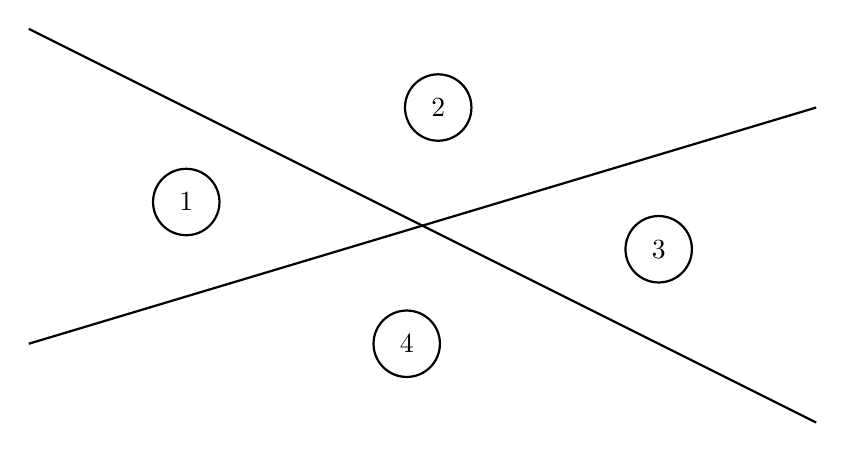
\begin{tikzpicture}[thick]
        \draw (-5,2.5) -- (5,-2.5);
        \draw (-5,-1.5) -- (5,1.5);
        \node[draw,circle,minimum size=24pt,inner sep=0,anchor=center] at (-0.2,-1.5) {$4$};
        \node[draw,circle,minimum size=24pt,inner sep=0,anchor=center] at (3,-0.3) {$3$};
        \node[draw,circle,minimum size=24pt,inner sep=0,anchor=center] at (-3,0.3) {$1$};
        \node[draw,circle,minimum size=24pt,inner sep=0,anchor=center] at (0.2,1.5) {$2$};
    \end{tikzpicture}
\end{center}

然而,这只是两条直线相交的一种\textit{具体情况}。我们怎么知道无论我们如何画这两条线,\textit{总能}得到四个区域?也就是说,我们能否以某种方式结合直线数量 $n = 2$ 这一事实来描述这是\text{如何}发生的?思考一下!

下面是我们的方法。请注意,当我们添加第二条直线时,每个已经存在的区域都会被分成两部分,并且\textit{无论你如何绘制直线},只要我们确保两条直线不平行,结果都是这样。也就是说,如果我们用一条直线将平面分成两个区域,

\begin{center}
    \begin{tikzpicture}[thick]
        \draw (-5,2.5) -- (5,-2.5);
        \node[draw,circle,minimum size=24pt,inner sep=0,anchor=center] at (-3,0.3) {$1$};
        \node[draw,circle,minimum size=24pt,inner sep=0,anchor=center] at (0.2,1.5) {$2$};
    \end{tikzpicture}
\end{center}

然后添加一条新的直线会将每个现有区域分成两部分。这会向整个平面添加两个新的区域,总共四个区域:

\begin{center}
    \begin{tikzpicture}[thick]
        \draw (-5,2.5) -- (5,-2.5);
        \draw [color=red] (-5,-1.5) -- (0,0)  node[midway,below,sloped]{分割区域 1}
        -- (5,1.5) node[midway,above,sloped]{分割区域 2} ;
        \node[draw,circle,minimum size=24pt,inner sep=0,anchor=center,color=red] at (-0.2,-1.5) {$4$};
        \node[draw,circle,minimum size=24pt,inner sep=0,anchor=center,color=red] at (3,-0.3) {$3$};
        \node[draw,circle,minimum size=24pt,inner sep=0,anchor=center] at (-3,0.3) {$1$};
        \node[draw,circle,minimum size=24pt,inner sep=0,anchor=center] at (0.2,1.5) {$2$};
    \end{tikzpicture}
\end{center}

当 $n = 3$ 时呢?在这种情况下,我们需要考虑向具有两条直线和四个区域的图形中添加第三条直线。我们想要提出一个不依赖于线的特定排列的论证,因此我们最终唯一能用的事实是线之间互不平行,且任何交点仅位于两条线(而不是三条或更多)上。不过,就目前而言,查看特定的线条排列会有所帮助,以便我们讨论相同的图形;我们可以利用对这个特定图形的观察来指导我们的一般论证。让我们从下方具有两条直线的图开始,向其中添加第三条线,我们让第三条线的交点都在初始交点“附近”或在图的范围内,这样我们就缩放图形了:

\begin{center}
    \begin{tikzpicture}[thick]
        \draw (-5,2.5) -- (5,-2.5);
        \draw (-5,-1.5) -- (5,1.5);
        \draw [color=red] (-5,1) -- (-1.8085,0.9043) node[midway,below,sloped]{\small 分割区域 1} 
        -- (2.5758,0.7727) node[midway,above,sloped]{\small 分割区域 2}
        -- (5,0.7) node[midway,below,sloped]{\small 分割区域 3};
        \node[draw,circle,minimum size=16pt,inner sep=0,anchor=center] at (-0.2,-1.5) {$4$};
        \node[draw,circle,minimum size=16pt,inner sep=0,anchor=center] at (3,-0.3) {$3$};
        \node[draw,circle,minimum size=16pt,inner sep=0,anchor=center] at (-3,-0.3) {$1$};
        \node[draw,circle,minimum size=16pt,inner sep=0,anchor=center] at (0.2,2) {$2$};
        \node[draw,circle,minimum size=16pt,inner sep=0,anchor=center,color=red] at (-4,1.45) {$5$};
        \node[draw,circle,minimum size=16pt,inner sep=0,anchor=center,color=red] at (0.1,0.45) {$6$};
        \node[draw,circle,minimum size=16pt,inner sep=0,anchor=center,color=red] at (4.61,1.05) {$7$};
    \end{tikzpicture}
\end{center}

很明显现在我们有 $7$ 个区域。我们将第三条线设置为不同的颜色,以便我们可以识别“新”区域出现的位置:一个区域(下方区域,区域 $4$)保持不变,但其他三个区域被一分为二,每个“分割”都会让我们的计数加 $1$(原来有 $1$ 个区域,现在有 $2$ 个)。如果我们以不同的方式绘制这条直线会怎样?

\begin{center}
    \begin{tikzpicture}[thick]
        \draw (-5,2.5) -- (5,-2.5);
        \draw (-5,-1.5) -- (5,1.5);
        \draw [color=red] (0,2.5) -- (-0.8333,0.4167) node[midway,right,sloped,rotate=-90]{\small 分割区域 2} 
        -- (-1.1364,-0.341) node[midway,left,sloped,rotate=-90]{\small 分割区域 1}
        -- (-2,-2.5) node[midway,right,sloped,rotate=-90]{\small 分割区域 4}; 
        \node[draw,circle,minimum size=16pt,inner sep=0,anchor=center] at (-0.2,-1) {$4$};
        \node[draw,circle,minimum size=16pt,inner sep=0,anchor=center] at (3,-0.3) {$3$};
        \node[draw,circle,minimum size=16pt,inner sep=0,anchor=center] at (-3,-0.3) {$1$};
        \node[draw,circle,minimum size=16pt,inner sep=0,anchor=center] at (1,2) {$2$};
        \node[draw,circle,minimum size=12pt,inner sep=0,anchor=center,color=red] at (-0.7,0.05) {$5$};
        \node[draw,circle,minimum size=16pt,inner sep=0,anchor=center,color=red] at (-1.5,1.8) {$6$};
        \node[draw,circle,minimum size=16pt,inner sep=0,anchor=center,color=red] at (-2.5,-1.4) {$7$};
    \end{tikzpicture}
\end{center}

同样的现象再次发生,其中一个区域保持不变,但其他三个区域一分为二。(我们怎么知道没有任何其他区域未绘制在我们这个比例的图形内?这并不像看上去的那么容易回答,值得深刻考虑。)尝试三条线的其他排列方式,并试图说服自己这种情况总会发生;此外,思考一下\textit{为什么}会出现这种情况,以及我们\textit{如何}解释这种情况一定会发生。不过,在给出一般性解释之前,我们先来看另一个小案例。

当 $n = 4$ 时,我们从 $3$ 条直线和 $7$ 个区域的平面开始,然后添加第四条直线,该线不与任何现有线平行,并且不穿过任何现有交点。同样,我们想要提出一个与特定的线条排列无关的论证,但是查看下面的具体图形将有助于引导我们的直觉来提出该论证:

\begin{center}
    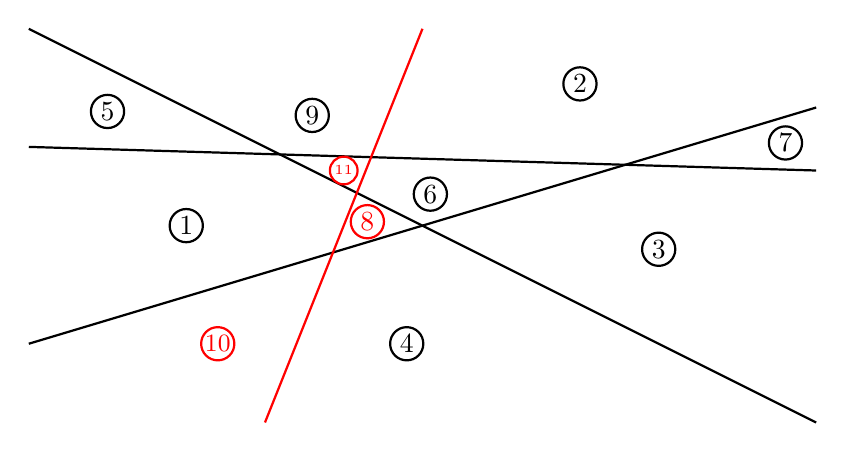
\begin{tikzpicture}[thick]
        \draw (-5,2.5) -- (5,-2.5);
        \draw (-5,-1.5) -- (5,1.5);
        \draw  (-5,1) -- (5,0.7);
        \draw [color=red] (0,2.5) -- (-2,-2.5);
        \node[draw,circle,minimum size=12pt,inner sep=0,anchor=center] at (-0.2,-1.5) {$4$};
        \node[draw,circle,minimum size=12pt,inner sep=0,anchor=center] at (3,-0.3) {$3$};
        \node[draw,circle,minimum size=12pt,inner sep=0,anchor=center] at (-3,0) {$1$};
        \node[draw,circle,minimum size=12pt,inner sep=0,anchor=center] at (2,1.8) {$2$};
        \node[draw,circle,minimum size=12pt,inner sep=0,anchor=center] at (-4,1.45) {$5$};
        \node[draw,circle,minimum size=12pt,inner sep=0,anchor=center] at (-1.4,1.4) {$9$};
        \node[draw,circle,minimum size=10pt,inner sep=0,anchor=center,color=red] at (-1,0.7) {\tiny $11$};
        \node[draw,circle,minimum size=12pt,inner sep=0,anchor=center] at (4.61,1.05) {$7$};
        \node[draw,circle,minimum size=12pt,inner sep=0,anchor=center,color=red] at (-0.7,0.05) {$8$};
        \node[draw,circle,minimum size=12pt,inner sep=0,anchor=center] at (0.1,0.4) {$6$};
        \node[draw,circle,minimum size=12pt,inner sep=0,anchor=center,color=red] at (-2.6,-1.5) {\small $10$};
    \end{tikzpicture}
\end{center}

请注意,三个原始区域保持不变(区域 $3$、区域 $5$ 和区域 $7$),其他四个区域一分为二。你注意到这里存在一个模式吗?似乎对于我们检查过的每个 $n$,添加第 $n$ 条线会使 $n-1$ 个区域保持不变,而其余区域则被一分为二。让我们尝试解释为什么会出现这种情况。请记住,当我们绘制 $n$ 条直线时,我们试图确定出现了多少个区域,因此让我们为该值分配一个“名称”,以便我们可以引用它;假设 $R(n)$ 表示在平面上绘制 $n$ 条直线所创建的区域数,且没有两条线平行,并且没有交点在两条以上的线上。在上面示例中,我们考虑了 $n$ 的较小取值,并研究了添加新的直线时会发生什么变化;也就是说,我们可以通过已知 $R(n - 1)$ 算出 $R(n)$ 的值。让我们整理一下我们的观察结果,以便它们适用于\textit{任意} $n$ 值。

假设我们已知 $R(n)$。(为什么我们可以这样做?对于某个特定的 $n$,我们是否确实知道 $R(n)$ 的特定值?这个值是什么?如何知道的?)假设我们在平面上有一个\textit{任意} $n$ 线图,满足上面题目陈述中给出的两个条件。这些直线创建了多少个区域?是的,正是 $R(n)$。现在,当我们添加第 $(n + 1)$ 条直线时会发生什么?关于这条线以及它如何改变图形,我们可以确定什么?其实,我们真正掌握的唯一信息是:

\begin{enumerate}[label=(\alph*)]
    \item 这条新的直线与现有的 $n$ 条直线中的任何一条都不平行;
    \item 这条新的直线不经过任何现有的交点。
\end{enumerate}

现在,条件 (a) 告诉我们这条新的直线必须与\textit{所有}现有的 $n$ 条直线线相交;平行线不相交,非平行线必然相交于某处。因此,我们必须在图上创建 $n$ 个新的交点。这些交点会与任何现有交点重合吗?不会!这正是条件 (b) 告诉我们的。这两条信息合在一起告诉我们,无论我们如何绘制这条新的直线,只要它满足题目的要求,这条直线上\textit{一定}会出现 $n$ 个“特殊”点。这些特殊点正是新线与现有线的交点。

我们现在想利用这些特殊点来识别图中的新区域。回顾一下我们上面研究的案例:识别新的交点,看看是否可以将它们与新的区域关联起来。也许用圆点标记这些交点并用 $\textbf{×}$ 标记新区域会有所帮助,让它们更容易辨认。我们在下面为你展示了一个示例,其中 $n = 4$。你注意到了什么?你能用这些点来帮助识别添加第 $n$ 条直线后创建了多少新区域吗?思考一下,然后继续阅读。

\begin{center}
    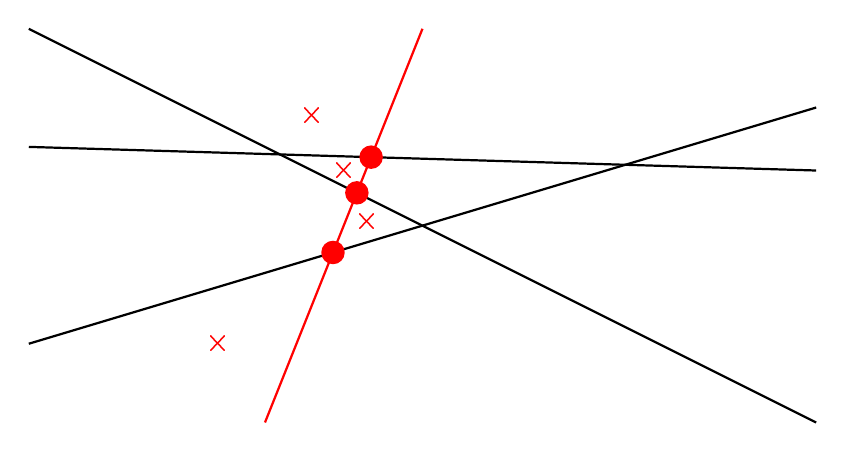
\begin{tikzpicture}[thick]
        \draw (-5,2.5) -- (5,-2.5);
        \draw (-5,-1.5) -- (5,1.5);
        \draw  (-5,1) -- (5,0.7);
        \draw [color=red] (0,2.5) -- (-2,-2.5);
        \node[minimum size=14pt,anchor=center,color=red,very thick] at (-1.4,1.4) {$\textbf{×}$};
        \node[minimum size=14pt,anchor=center,color=red,very thick] at (-1,0.7) {$\textbf{×}$};
        \node[minimum size=14pt,anchor=center,color=red,very thick] at (-0.7,0.05) {$\textbf{×}$};
        \node[minimum size=14pt,anchor=center,color=red,very thick] at (-2.6,-1.5) {$\textbf{×}$};
        \node[fill,circle,inner sep=3pt,color=red] at (-0.6522,0.8696) {};
        \node[fill,circle,inner sep=3pt,color=red] at (-0.8333,0.4167) {};
        \node[fill,circle,inner sep=3pt,color=red] at (-1.1364,-0.341) {};
    \end{tikzpicture}
\end{center}

没错!任意两个相邻新交点之间,都有一条\textit{线段}将一个区域一分为二!剩下的就是确定我们创建了多少个新的此类线段。由于每条线段都将唯一\textit{一个}现有区域一分为二,因此这将准确地告诉我们创建了多少个新区域。我们已知,第 $(n + 1)$ 条直线线创建了 $n$ 个新的交点。想想这些点是如何排列在直线上的。任意两个“连续”点都会创建一条线段,但极点也会创建无限线段(永远延申下去经过这些极点)。总共有多少个?正好是 $n + 1$。(参考上图,$n = 3$。我们看到有 $3$ 个新交点和 $4$ 条新线段,其中两个是无限射线。)这意味着有 $n + 1$ 条线段将区域一分为二,因此我们恰好创建了 $n + 1$ 个新区域!这让我们可以说
\[R(n + 1) = R(n) + n + 1\]
哇,多好的观察啊!我们花了一些时间研究示例并进行了一些几何论证,但最终我们做到了。我们已经确定了这个问题的一些归纳结构;我们发现一个情况如何依赖另一个情况。也就是说,我们发现了 $R(n+1)$ 如何依赖 $R(n)$。这还没有完全解决这个问题,但我们现在已经非常接近了。剩下的就是用类似的表达式替换 $R(n)$,并不断执行此操作,直到达到我们已知的 $R(1) = 2$。观察:

\begin{center}
    \begin{tabular}{rcccccccccc}
        $R(n+1)$ & $=$ &          & &            &     &            &     & $\cancel{R(n-1)}$ & $+$ & $n+1$\\
                 & $=$ &          & &                   &     & $\cancel{R(n-1)}$ & $+$ & $n$ & $+$ & $n+1$\\
                 & $=$ &          & & $\cancel{R(n-2)}$ & $+$ & $(n-1)$           & $+$ & $n$ & $+$ & $n+1$\\
                 & $\vdots$ &     & &  &  &  &  &  &  & \\
                 & $=$ &          & & $\cancel{R(2)}+3$ & $+$ & $\dots$ & $+$ & $n$ & $+$ & $n+1$ \\
                 & $=$ & $R(1)+2$ & $+$ & $3$               & $+$ & $\dots$ & $+$ & $n$ & $+$ & $n+1$ \\
    \end{tabular}
\end{center}

因为我们知道 $R(1) = 2$,所以我们可以说
\[R(n + 1) = 2 + \big(2 + 3 + \dots + n + (n + 1)\big) = 2 + \Bigg(\sum_{k=1}^{n+1}k\Bigg)-1 = 1+\sum_{k=1}^{n+1}k\]
而这正是我们之前研究过的求和公式!(另请注意,我们必须减去 $1$,因为括号中缺少求和的第一项。)回想一下 $\sum_{k=1}^{n} k = \frac{n(n+1)}{2}$,为了表示上面等式中的求和,我们只需将 $n$ 替换为 $n + 1$ 即可。因此,
\[R(n + 1) = 1+\frac{(n+1)(n+2)}{2}\]
我们要进行的最后一步简化是将整个方程中的 $n+1$ 替换为 $n$,因为使用 $R(n)$ 的表达式更有意义(对 $n$ 的值有什么要求?)
\[R(n + 1) = 1+\frac{n(n+1)}{2}\]
最终,我们找到了开头问题的答案!在这个过程中,我们采用了\textit{归纳}技术:我们解释了一个“事实”(即 $R(n + 1)$ 的值)如何\textit{取决于}“前一个事实”(即 $R(n)$ 的值),并使用这些迭代依赖关系进行反向运算,直到达到一个特定的\textit{已知}值,即 $R(1)$。

我们想再次指出,我们在本节中所做的推导和观察只是引导我们的直觉从而得出答案,并不是\textit{严格证明}。问题出在 “$\dots$” 身上,省略号不是具体的、“官方”的数学方法来捕获归纳技术背后的归纳过程。此外,我们解决“平面中的线”问题的方法是从 $n - 1$ 条线的图形\textit{开始,构建}一个包含 $n$ 条线的新图;这样可以吗?为什么这实际上告诉了我们有关 $n$ 条线的\textit{任意}图的信息?所有这些图都来自于少了一条线的较小图吗?

在接下来的两章中,我们将学习必要的工具来充分描述我们迄今为止所做事情的严格方法,在那之后的章节中,我们将使用这些工具让数学归纳法变得正式而严谨。不过,现在我们想给出归纳法的启发式定义,并继续研究依赖归纳技术的有趣问题和观察结果。练习这些类型的问题 --- 学习何时识别归纳过程、如何使用它、如何使用该结构来解决问题等等 --- 将在未来非常有帮助,我们不需要深入到数学技术细节。(至少,现在还不需要!)

\subsection{问题与练习}

\subsubsection*{提醒自己}

口头或书面简要回答以下问题。这些题目全都基于你刚刚阅读的部分,因此如果你无法想起特定的定义、概念或示例,请返回重新阅读相应部分。确保自己在继续之前可以自信地回答这些问题,这将有助于你的理解和记忆!

\begin{enumerate}[label=(\arabic*)]
    \item 归纳过程有哪些特征?
    \item 我们如何证明 $\sum_{k=1}^{n}k = \frac{n(n+1)}{2}$ 是正确的?我们的方法是如何归纳的?(如果你不记得了,请重读第 \ref{sec:section1.4.2} 节!)
    \item 为什么我们可以把上一个问题中提到的求和公式,用 $n+1$ “替换” $n$,并且知道它仍然成立?我们也可以将 $n$ 替换为 $n - 1$ 吗?
    \item 通过代数步骤获得前 $n$ 个自然数平方和的最终表达式;也就是说,验证
    \[\frac{1}{3}(n+1)^3-\frac{1}{3}(n+1)-\frac{n(n+1)}{2} = \frac{1}{6}n(n+1)(2n+1)\]
    \item 试着回忆一下向平面中添加第 $(n+1)$ 条直线正好会创建 $n+1$ 个新区域的论点。你能为朋友证明这个论点并说服他/她它是有效的吗?
    \item 求前 $n$ 个自然数的平方和,为什么不能把前 $n$ 个自然数之和的公式平方呢?为什么这是错误的?
\end{enumerate}

\subsubsection*{试一试}

尝试回答以下简答题。这些题目要求你实际动笔写一写,或(对朋友/同学)口头描述一些东西。目的是让你练习使用新概念、定义和符号。别担心,这些题本来就很简单。确保能够解决这些问题将对你有所帮助!

\begin{enumerate}[label=(\arabic*)]
    \item 在平面中画 $5$ 条直线(满足原题的两个条件)并验证是否有 $16$ 个区域。你还能验证 $6$ 条线产生 $22$ 个区域吗?
    \item 给出序列 $1, 2, 3, 4, \dots , 100$ 的另一种解释,而不仅仅是从 $1$ 到 $100$ 的所有自然数。(回想一下我们给出的例子:$1$ 到 $100$ 之间所有英文拼写中不含字母"i"的数字。)
    \item 提出一个将 $(n + 1)^4$ 与 $n^4$ 联系起来的代数表达式,就像我们对立方所做的那样。\\ 
    (\textbf{挑战题:}你能为刚刚推导出的表达式给出\textit{几何}解释吗?)
    \item \textbf{挑战题:}让我们将“平面上的线”这题提升一个维度!考虑三维空间中有 $n$ 个平面。会创建多少个区域?假设没有两个平面平行,并且没有三个或以上平面相交于一条直线。(想想这两个条件如何直接类比于“线”那题的给定条件。)
\end{enumerate}

\newpage
% !TeX root = ../../book.tex
\section{定义归纳}

\newpage
% !TeX root = ../../book.tex
\section{另外两个(不同)的例子}

这一小节有几个目的。首先,我们不希望你认为归纳法就是用数字和多项式证明一个\textit{数值公式}。归纳法比那有用得多!尤其是下面一个例子,证明了某些抽象属性对于给定情况的任何``大小''都成立。你将看到它仍然属于``归纳''的范畴,但你也会注意到它与前面示例的不同之处。此外,这些例子还说明,有时我们需要了解``更多信息''才能将多米诺骨牌推到。在先前的例子中,我们只需要知道骨牌 $n$ 倒下就可以\textit{保证}骨牌 $n + 1$ 倒下。但在本节的示例中,我们可能需要了解之前几张多米诺骨牌。在这两个例子之后,我们会总结这与先前给出的多米诺骨牌定义有何不同,并预览归纳技术的更通用的定义,因为它适用于这些例子。

\subsection{多米诺与密铺}

下面的示例比前两个示例稍微复杂一些。我们最终仍将证明某个数值公式,但问题显然比仅仅操纵代数表达式更加直观。此外,我们会在开始步骤中注意到一个有趣的``问题'',即我们必须解决几个``小案例'',然后才能推广我们的方法。这将是我们首次考虑如何泛化归纳技术使其适应其他情况。

我们要回答的问题可以表述如下:

\begin{quote}
    给定一个 $2 \times n$ 的正方形棋盘,有多少种不同的方式可以用多米诺骨牌平铺该棋盘?平铺必须让每个正方形都被一块——且只有一块——多米诺骨牌覆盖。
\end{quote}
例如,以下是正确的密铺

\begin{center}
    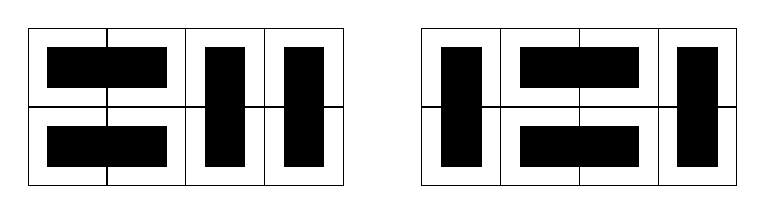
\begin{tikzpicture}[x=1.0cm, y=1.0cm]
        \foreach \y in {0,1} {
            \foreach \x in {0,...,3} {
                \draw (0+\x ,0+\y) rectangle ++ (1,1);
            }
        }

        \draw[fill, black] (0.25 ,0.25) rectangle ++ (1.5,0.5);
        \draw[fill, black] (0.25 ,1.25) rectangle ++ (1.5,0.5);
        \draw[fill, black] (2.25 ,0.25) rectangle ++ (0.5,1.5);
        \draw[fill, black] (3.25 ,0.25) rectangle ++ (0.5,1.5);

        \foreach \y in {0,1} {
            \foreach \x in {0,...,3} {
                \draw (5+\x ,0+\y) rectangle ++ (1,1);
            }
        }

        \draw[fill, black] (5+1.25 ,0.25) rectangle ++ (1.5,0.5);
        \draw[fill, black] (5+1.25 ,1.25) rectangle ++ (1.5,0.5);
        \draw[fill, black] (5+0.25 ,0.25) rectangle ++ (0.5,1.5);
        \draw[fill, black] (5+3.25 ,0.25) rectangle ++ (0.5,1.5);
    \end{tikzpicture}
\end{center}
而以下\textit{不}是正确的密铺

\begin{center}
    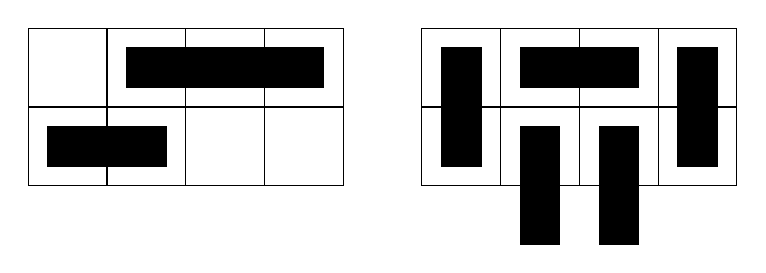
\begin{tikzpicture}[x=1.0cm, y=1.0cm]
        \foreach \y in {0,1} {
            \foreach \x in {0,...,3} {
                \draw (0+\x ,0+\y) rectangle ++ (1,1);
            }
        }

        \draw[fill, black] (0.25 ,0.25) rectangle ++ (1.5,0.5);
        \draw[fill, black] (1.25 ,1.25) rectangle ++ (1.5,0.5);
        \draw[fill, black] (2.25 ,1.25) rectangle ++ (1.5,0.5);

        \foreach \y in {0,1} {
            \foreach \x in {0,...,3} {
                \draw (5+\x ,0+\y) rectangle ++ (1,1);
            }
        }

        \draw[fill, black] (5+1.25 ,1.25) rectangle ++ (1.5,0.5);
        \draw[fill, black] (5+1.25 ,-0.75) rectangle ++ (0.5,1.5);
        \draw[fill, black] (5+2.25 ,-0.75) rectangle ++ (0.5,1.5);
        \draw[fill, black] (5+0.25 ,0.25) rectangle ++ (0.5,1.5);
        \draw[fill, black] (5+3.25 ,0.25) rectangle ++ (0.5,1.5);
    \end{tikzpicture}
\end{center}

和以前一样,让我们查看前几种情况(其中 $n = 1, 2, 3$ 等),看看我们是否能发现任何模式。在继续阅读之前,尝试自己解决该问题!

当 $n = 1$ 时,我们有一个与多米诺骨牌形状完全相同的棋盘,因此肯定只有一种方法可以密铺。让我们使用符号 $T(n)$ 来表示 $2 \times n$ 棋盘上的密铺数量。因此,$T(1) = 1$。

\begin{center}
    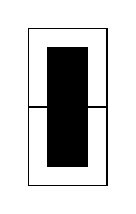
\begin{tikzpicture}[x=1.0cm, y=1.0cm]
        \draw (0,0) rectangle ++ (1,1);
        \draw (0,1) rectangle ++ (1,1);
        \draw[fill, black] (0.25 ,0.25) rectangle ++ (0.5,1.5);
    \end{tikzpicture}
\end{center}
当 $n = 2$ 时,我们有一个 $2 \times 2$ 棋盘。由于棋盘的方向很重要,因此我们有以下两种不同的密铺。因此,$T(2) = 2$。

\begin{center}
    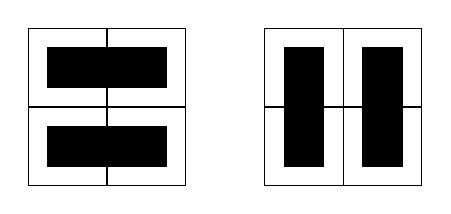
\begin{tikzpicture}[x=1.0cm, y=1.0cm]
        \foreach \y in {0,1} {
            \foreach \x in {0,1} {
                \draw (0+\x ,0+\y) rectangle ++ (1,1);
            }
        }

        \draw[fill, black] (0.25 ,0.25) rectangle ++ (1.5,0.5);
        \draw[fill, black] (0.25 ,1.25) rectangle ++ (1.5,0.5);

        \foreach \y in {0,1} {
            \foreach \x in {0,1} {
                \draw (3+\x ,0+\y) rectangle ++ (1,1);
            }
        }

        \draw[fill, black] (3+0.25 ,0.25) rectangle ++ (0.5,1.5);
        \draw[fill, black] (3+1.25 ,0.25) rectangle ++ (0.5,1.5);
    \end{tikzpicture}
\end{center}
当 $n = 3$ 时呢?同样地,我们可以手动枚举这些密铺,并确保没有遗漏任何一个。我们看到 $T(3) = 3$。

\begin{center}
    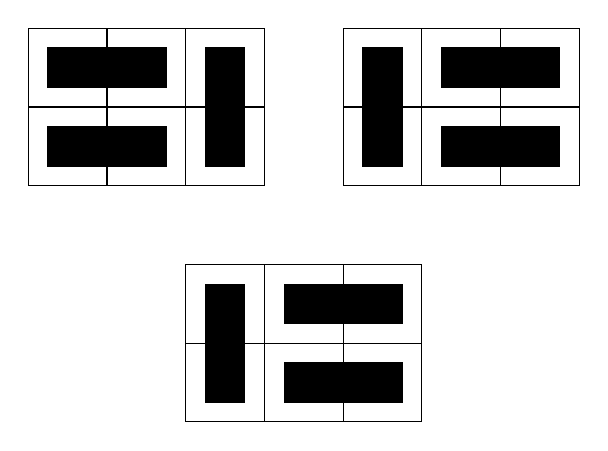
\begin{tikzpicture}[x=1.0cm, y=1.0cm]
        \foreach \y in {0,1} {
            \foreach \x in {0,1,2} {
                \draw (0+\x ,0+\y) rectangle ++ (1,1);
            }
        }

        \draw[fill, black] (0.25 ,0.25) rectangle ++ (1.5,0.5);
        \draw[fill, black] (0.25 ,1.25) rectangle ++ (1.5,0.5);
        \draw[fill, black] (2.25 ,0.25) rectangle ++ (0.5,1.5);

        \foreach \y in {0,1} {
            \foreach \x in {0,1,2} {
                \draw (4+\x ,0+\y) rectangle ++ (1,1);
            }
        }

        \draw[fill, black] (4+1.25 ,0.25) rectangle ++ (1.5,0.5);
        \draw[fill, black] (4+1.25 ,1.25) rectangle ++ (1.5,0.5);
        \draw[fill, black] (4+0.25 ,0.25) rectangle ++ (0.5,1.5);

        \foreach \y in {0,1} {
            \foreach \x in {0,1,2} {
                \draw (2+\x ,-3+\y) rectangle ++ (1,1);
            }
        }

        \draw[fill, black] (2+1.25 ,-3+0.25) rectangle ++ (1.5,0.5);
        \draw[fill, black] (2+1.25 ,-3+1.25) rectangle ++ (1.5,0.5);
        \draw[fill, black] (2+0.25 ,-3+0.25) rectangle ++ (0.5,1.5);
    \end{tikzpicture}
\end{center}
好的,再看一种情况,当 $n=4$ 时,我们看到 $T(4)=5$。

\begin{center}
    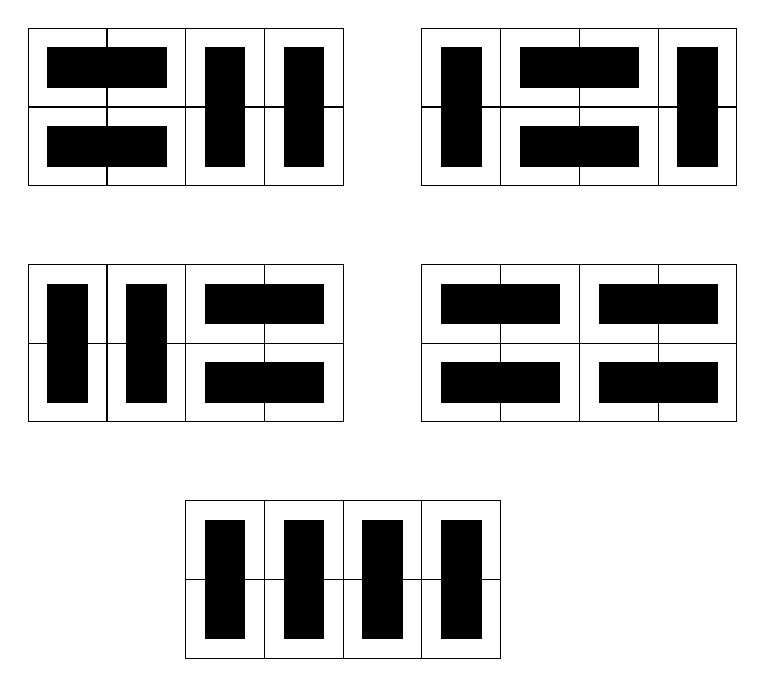
\begin{tikzpicture}[x=1.0cm, y=1.0cm]
        \foreach \y in {0,1} {
            \foreach \x in {0,...,3} {
                \draw (0+\x ,0+\y) rectangle ++ (1,1);
            }
        }

        \draw[fill, black] (0.25 ,0.25) rectangle ++ (1.5,0.5);
        \draw[fill, black] (0.25 ,1.25) rectangle ++ (1.5,0.5);
        \draw[fill, black] (2.25 ,0.25) rectangle ++ (0.5,1.5);
        \draw[fill, black] (3.25 ,0.25) rectangle ++ (0.5,1.5);

        \foreach \y in {0,1} {
            \foreach \x in {0,...,3} {
                \draw (5+\x ,0+\y) rectangle ++ (1,1);
            }
        }

        \draw[fill, black] (5+1.25 ,0.25) rectangle ++ (1.5,0.5);
        \draw[fill, black] (5+1.25 ,1.25) rectangle ++ (1.5,0.5);
        \draw[fill, black] (5+0.25 ,0.25) rectangle ++ (0.5,1.5);
        \draw[fill, black] (5+3.25 ,0.25) rectangle ++ (0.5,1.5);

        \foreach \y in {0,1} {
            \foreach \x in {0,...,3} {
                \draw (0+\x ,-3+\y) rectangle ++ (1,1);
            }
        }

        \draw[fill, black] (2.25 ,-3+0.25) rectangle ++ (1.5,0.5);
        \draw[fill, black] (2.25 ,-3+1.25) rectangle ++ (1.5,0.5);
        \draw[fill, black] (0.25 ,-3+0.25) rectangle ++ (0.5,1.5);
        \draw[fill, black] (1.25 ,-3+0.25) rectangle ++ (0.5,1.5);

        \foreach \y in {0,1} {
            \foreach \x in {0,...,3} {
                \draw (5+\x ,-3+\y) rectangle ++ (1,1);
            }
        }

        \draw[fill, black] (5+2.25 ,-3+0.25) rectangle ++ (1.5,0.5);
        \draw[fill, black] (5+2.25 ,-3+1.25) rectangle ++ (1.5,0.5);
        \draw[fill, black] (5+0.25 ,-3+0.25) rectangle ++ (1.5,0.5);
        \draw[fill, black] (5+0.25 ,-3+1.25) rectangle ++ (1.5,0.5);

        \foreach \y in {0,1} {
            \foreach \x in {0,...,3} {
                \draw (2+\x ,-6+\y) rectangle ++ (1,1);
            }
        }

        \draw[fill, black] (2+0.25 ,-6+0.25) rectangle ++ (0.5,1.5);
        \draw[fill, black] (2+1.25 ,-6+0.25) rectangle ++ (0.5,1.5);
        \draw[fill, black] (2+2.25 ,-6+0.25) rectangle ++ (0.5,1.5);
        \draw[fill, black] (2+3.25 ,-6+0.25) rectangle ++ (0.5,1.5);
    \end{tikzpicture}
\end{center}

我们现在可以开始寻找模式了吗?找到更大棋盘的密铺会很繁琐!让我们考虑一下如何利用 $T(1) = 1$ 的事实来推断出有关 $T(2)$ 的信息……等一下……做不到,对吧?这两个案例有本质的区别。具体来说,由于多米诺骨牌的大小为 $2 \times 1$,因此我们仅向棋盘中添加一行这一事实对我们没有帮助。

好吧,那么我们考虑 $n = 3$。我们可以利用 $T(2) = 2$ 这个事实吗?在这种情况下,答案是肯定的!知道 $2 \times 2$ 棋盘有两个密铺,无需太多思考,我们可以立即构建 $2 \times 3$ 棋盘的两个平铺。具体来说,我们可以将\textit{垂直多米诺骨牌添加}到之前的每一个密铺中。但我们知道 $T(3) = 3$。第三个密铺从何而来?再次查看该密铺,以及它与其他两个密铺的比较。在第三个密铺中,右侧的多米诺骨牌是水平的,而不是其他两种密铺中的垂直多米诺骨牌。如果我们移除这两个平行的水平多米诺骨牌,我们就会得到 $n = 1$ 时的情况。换句话说,我们可以通过在右侧\textit{添加一个由两个水平多米诺骨牌组成的正方形}来构建 $2 \times 3$ 棋盘的密铺。总的来说,我们已经用较小尺寸的棋盘(即 $2 \times 2$ 和 $2 \times 1$)描述了 $2 \times 3$ 棋盘的所有密铺:

\begin{center}
    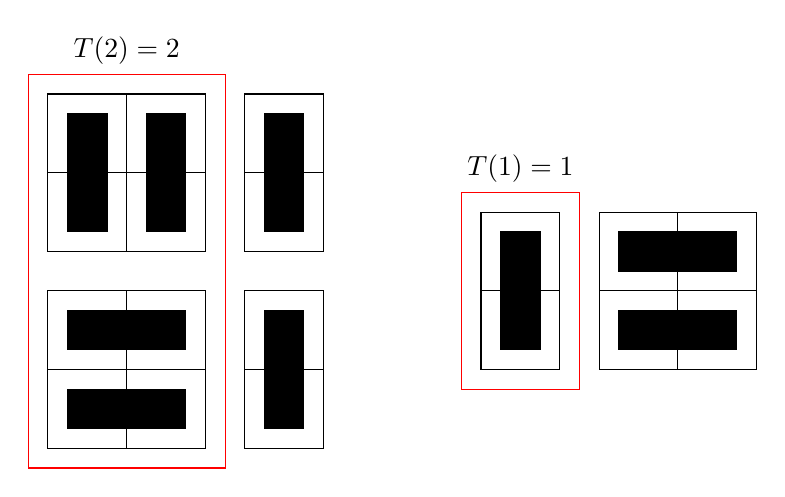
\begin{tikzpicture}[x=1.0cm, y=1.0cm]
        \foreach \g in {0, 2.5} {
            \foreach \y in {0,1} {
                \foreach \x in {0,1} {
                    \draw (0+\x ,0+\y+\g) rectangle ++ (1,1);
                }
            }
            \draw (2.5,0+\g) rectangle ++ (1,1);
            \draw (2.5,1+\g) rectangle ++ (1,1);
            \draw[fill, black] (2.75 ,0.25+\g) rectangle ++ (0.5,1.5);
        }

        \draw[fill, black] (0.25 ,0.25) rectangle ++ (1.5,0.5);
        \draw[fill, black] (0.25 ,1.25) rectangle ++ (1.5,0.5);

        \draw[fill, black] (0.25 ,2.5+0.25) rectangle ++ (0.5,1.5);
        \draw[fill, black] (1.25 ,2.5+0.25) rectangle ++ (0.5,1.5);

        \draw[red] (-0.25, -0.25) rectangle ++(2.5, 5);
        \path (-0.25,4.75) --  (2.25,4.75) node[midway,above,black] {$T(2)=2$};

        \draw (5.5,1) rectangle ++ (1,1);
        \draw (5.5,2) rectangle ++ (1,1);
        \draw[fill, black] (5.75 ,1.25) rectangle ++ (0.5,1.5);
        \draw[red] (5.25, 0.75) rectangle ++(1.5, 2.5);
        \path (5.25,3.25) --  (6.75,3.25) node[midway,above,black] {$T(1)=1$};

        \foreach \y in {0,1} {
            \foreach \x in {0,1} {
                \draw (7+\x ,1+\y) rectangle ++ (1,1);
            }
        }
        \draw[fill, black] (7.25 ,1.25) rectangle ++ (1.5,0.5);
        \draw[fill, black] (7.25 ,2.25) rectangle ++ (1.5,0.5);

    \end{tikzpicture}
\end{center}
\[T(3) = 3 = 2 + 1 = T(2) + T(1)\]

现在你可能会看出模式来!我们再看一下当 $n = 4$ 时会发生什么,我们将垂直多米诺骨牌添加到构成 $T(3)$ 的每一个密铺中,或者将两个水平多米诺骨牌添加到构成 $T(2)$ 的每一个密铺中,以此得到 $T(4)$ 的\textit{所有}密铺:

\begin{center}
    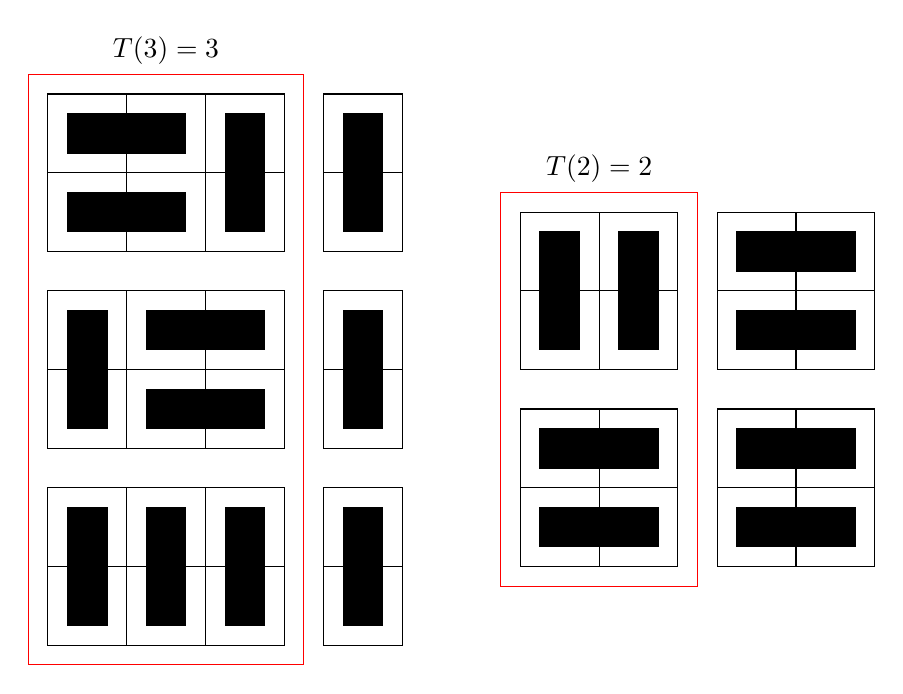
\begin{tikzpicture}[x=1.0cm, y=1.0cm]
        \foreach \g in {0, 2.5, 5} {
            \foreach \y in {0,1} {
                \foreach \x in {0,1,2} {
                    \draw (0+\x ,0+\y+\g) rectangle ++ (1,1);
                }
            }

            \draw (3.5,\g+0) rectangle ++ (1,1);
            \draw (3.5,\g+1) rectangle ++ (1,1);
            \draw[fill, black] (3.75 ,\g+0.25) rectangle ++ (0.5,1.5);
        }
        \draw[fill, black] (0.25 ,0.25) rectangle ++ (0.5,1.5);
        \draw[fill, black] (1.25 ,0.25) rectangle ++ (0.5,1.5);
        \draw[fill, black] (2.25 ,0.25) rectangle ++ (0.5,1.5);

        \draw[fill, black] (0.25 ,2.75) rectangle ++ (0.5,1.5);
        \draw[fill, black] (1.25 ,2.75) rectangle ++ (1.5,0.5);
        \draw[fill, black] (1.25 ,3.75) rectangle ++ (1.5,0.5);

        \draw[fill, black] (2.25 ,5.25) rectangle ++ (0.5,1.5);
        \draw[fill, black] (0.25 ,5.25) rectangle ++ (1.5,0.5);
        \draw[fill, black] (0.25 ,6.25) rectangle ++ (1.5,0.5);

        \draw[red] (-0.25, -0.25) rectangle ++(3.5, 7.5);
        \path (-0.25,7.25) --  (3.25,7.25) node[midway,above,black] {$T(3)=3$};


        \foreach \g in {0, 2.5} {
            \foreach \y in {0,1} {
                \foreach \x in {0,1} {
                    \draw (6+\x ,1+\y+\g) rectangle ++ (1,1);
                }
            }
            \foreach \y in {0,1} {
                \foreach \x in {0,1} {
                    \draw (8.5+\x ,1+\y+\g) rectangle ++ (1,1);
                }
                \draw[fill, black] (8.75 ,1.25+\g+\y) rectangle ++ (1.5,0.5);
            }
           
        }

        \draw[fill, black] (6.25 ,1.25) rectangle ++ (1.5,0.5);
        \draw[fill, black] (6.25 ,2.25) rectangle ++ (1.5,0.5);

        \draw[fill, black] (6.25 ,3.5+0.25) rectangle ++ (0.5,1.5);
        \draw[fill, black] (7.25 ,3.5+0.25) rectangle ++ (0.5,1.5);

        \draw[red] (5.75, 0.75) rectangle ++(2.5, 5);
        \path (5.75,5.75) --  (8.25,5.75) node[midway,above,black] {$T(2)=2$};
        
    \end{tikzpicture}
\end{center}
\[T(4) = 5 = 3 + 2 = T(3) + T(2)\]

另请注意,用这种方式不会产生重复的 $2 \times 4$ 密铺。(仔细想想为什么会这样。我们用一种什么方法表征两种密铺可以保证它们不重复?)有了这些信息,我们可以立即得出结论 $T(4) = T(3) + T(2)$。

此外,我们可以概括这样一个论点;$n = 4$ 没有什么特别的,对吧?对于任意特定的 $n$,我们可以只考虑所有可能的密铺,然后看看棋盘\textit{最右侧}发生的情况:要么有一个垂直多米诺骨牌(这意味着密铺来自 $2 \times (n - 1)$ 棋盘),要么有两个水平多米诺骨牌(这意味着密铺来自 $2 \times (n-2)$ 棋盘)。有了这个论点的支撑,对于所有有意义的 $n$ 值,我们可以得出如下结论:
\[T(n) = T(n - 1) + T(n - 2)\]
哪些 $n$ 值有意义?请记住,我们必须单独分析 $T(1)$ 和 $T(2)$;因此这个论点不适用于 $n=1$ 和 $n=2$,我们必须添加限制条件 $n \ge 3$ 才能使上面公式成立。

有了这些信息,只要有足够的时间,我们就可以轻松计算出任意 $n$ 值下的 $T(n)$。我们甚至可以相当容易地编写出计算机程序。然而,正是这种\textit{归纳}论证——我们注意到的模式以及我们对其发生原因的彻底描述——让我们首先得出了结论。这种情况下,每一项的值 $T(n)$ 取决于前\textit{两}项 $T(n-1)$ 和 $T(n-2)$ 的值。这在本章之前的例子中\textit{没有}出现过,它暗示了这里发生了更深层次的事情。你是否发现我们之前对归纳的定义以及多米诺骨牌的类比在这里不再适用?你会如何修正我们的类比来解释这种情况?思考一下这些问题,然后继续阅读。我们将在下一个示例之后更深入地讨论它们。

顺便一提,你是否注意到此示例的解有一些有趣的地方?你还知道其他类似的数列吗?想一想……

\subsection{制胜策略}

这个例子将是我们第一个\textit{无需}证明数值公式的归纳问题!这似乎很奇怪,但正如即将看到的那样,这却是一个事实。实际上在数学中,这比你想象的更常见:一个问题或数学对象可能存在某些潜在的归纳结构,但却不依赖代数或算术的内容。

事实上,我们将讨论一个\textit{游戏}。就是通常意义上的游戏——有两个玩家必须遵守的规则,并且有明显的赢家和输家——同时也是数学意义上的游戏,我们可以使用数学符号来制定规则和游戏情境,并以抽象的方式讨论\textit{策略}。我们甚至可以\textit{解}这个游戏。这与棒球比赛非常不同。

现在让我们讨论一下这个游戏的规则,我们暂时将其称为``取石子''。有两个玩家,称为 $P_1$ 和 $P_2$。玩家 $P_1$ 先行。玩家面前的桌子上有两堆石子,每堆正好有 $n$ 个石子,其中 $n$ 是某个自然数。(为了区分游戏的不同版本,当每堆石子有 $n$ 个石子时,我们会说玩家正在``玩 $T_n$''。)在每个玩家的回合中,他们可以从\textit{任意}一堆中取走\textit{任意}数量的石子。但不能同时从两堆石子中取石子。取走\textit{最后}一颗石子的玩家\textit{获胜}。

试着跟朋友玩一下这个游戏。使用硬币或糖果当石子。再试着切换一下角色,你先作为 $P_1$,然后再作为 $P_2$。尝试制定一个获胜\textit{策略},一种最大化获胜机会的游戏方法。尝试猜测不同的 $n$ 值下会发生什么。谁``应该''获胜?你能\textit{证明}吗?说真的,在继续阅读我们的分析之前,先玩玩这个游戏并尝试证明一些结论。你可能会对自己所取得的成就感到惊讶!

与其他示例一样,让我们使用 $n$ 的一些较小值来弄清楚到底发生了什么,然后再尝试进行泛化。当 $n = 1$ 时,这个游戏相当愚蠢。$P_1$ 必须取走其中一堆中唯一的石子,然后 $P_2$ 取走另一堆中唯一剩余的石子。因此,$P_2$ 胜。(请注意,无论 $P_1$ 选择两堆中的哪一堆,$P_2$ 总是会得到另一堆。我们可以说``不失一般性'', $P_1$ 选择左边这堆,因为无论选择哪一堆都无关紧要;情况是等价的,所以为了方便具体讨论,我们不妨说是左边这堆。后面讨论数理逻辑时,我们也会深入探讨``不失一般性''这一思想。)


\begin{center}
    \begin{tikzpicture}[line width=0.5mm]
        \foreach \n in {0, 1}{
            \node at (\n, 0)[circle,fill,inner sep=8pt, anchor=west]{};
            \draw (\n, -1) -- +(0.8, 0);
        }
        \draw[-latex] (2.5, -0.4) -- +(2, 0) node[midway,above]{$P_1$ 回合};
        \draw (5, -1) -- +(0.8, 0);
        \node at (6, 0)[circle,fill,inner sep=8pt, anchor=west]{};
        \draw (6, -1) -- +(0.8, 0);
        \draw[-latex] (7.5, -0.4) -- +(2, 0) node[midway,above]{$P_2$ 回合};
        \draw (10, -1) -- +(0.8, 0);
        \draw (11, -1) -- +(0.8, 0);
        \path (10, -0.4) -- +(2, 0) node[midway,above]{$P_2$ 胜!};
    \end{tikzpicture}
\end{center}

当 $n = 2$ 时,可能会出现几种情况。思考 $P_1$ 可能采取的行动。同样地,$P_1$ 可能选择左堆也可能选择右堆,但因为最终结果是相同的,并且我们可以交换这两堆,所以我们可以说(不失一般性)$P_1$ 从左堆取走若干石子。具体是多少?可能是一颗石子也可能是两颗石子。让我们分别检验每种情况。

\begin{center}
    \begin{tikzpicture}[line width=0.5mm]
        \foreach \x in {0, 1}{
            \node at (\x, 0)[circle,fill,inner sep=8pt, anchor=west]{};
            \node at (\x, 1)[circle,fill,inner sep=8pt, anchor=west]{};
            \draw (\x, -1) -- +(0.8, 0);
        }
        \draw[-latex] (2.5, -0.4) -- +(2, -0.6);
        \draw[-latex] (2.5, 0.6) -- +(2, 0.6);
        \node[anchor=west] at(2.5,0) {$P_1$ 回合};
        \foreach \delta in {1, -2}{
            \foreach \n in {0, 1}{
                \draw (5+\n, \delta) -- +(0.8, 0);
                \node at (6, \delta+1+\n)[circle,fill,inner sep=8pt, anchor=west]{};
            }
        }
        \node at (5, -1)[circle,fill,inner sep=8pt, anchor=west]{};
        \draw[-latex] (7.5, 2) -- +(2, 0) node[midway,above]{$P_2$ 回合};
        \draw[-latex] (7.5, -1) -- +(2, 0) node[midway,above]{$P_2$ 回合};
        \draw (10, 1) -- +(0.8, 0);
        \draw (11, 1) -- +(0.8, 0);
        \path (10, 1.6) -- +(2, 0) node[midway,above]{$P_2$ 胜!};
        \path (10, -1.4) -- +(2, 0) node[midway,above]{???};
    \end{tikzpicture}
\end{center}

如果 $P_1$ 取走两颗石子,$P_2$ 应该如何应对呢?$P_2$ 可以取走另一堆从而获胜,所以 $P_1$ 一开始就不应该采取这一行动。不过,可能 $P_1$ 脑子不清什么的,而且我们需要考虑所有可能的情况来全面分析这场比赛。因此,在这种情况下(上图中的上半行)$P_2$ 获胜。好吧,这就是简单的情况。

如果 $P_1$ 只从左边一堆石子(上图中的下半行)中取走一颗石子怎么办?$P_2$ 应该如何应对?我们现在有几种选择:

\begin{itemize}
    \item 如果 $P_2$ 从左边一堆石子中取走另一颗石子……那么,$P_2$ 取走另一堆全部石子,$P_1$ 获胜。
    \item 如果 $P_2$ 从右边一堆石子中取走全部两颗石子……那么,$P_1$ 取走左边一堆中的最后一颗石子,$P_1$ 获胜。
    \item 然而,如果 $P_2$ 只从右边一堆石子中取走一颗石子……
\end{itemize}

\begin{center}
    \begin{tikzpicture}[line width=0.5mm]
        \foreach \g in {0, 5, 10} {
            \foreach \x in {0, 1} {
                \node at (\x+\g, 0)[circle,fill,inner sep=8pt, anchor=west]{};
                \draw (\x+\g, -1) -- +(0.8, 0);
            }
        }
        \node at (0, 1)[circle,fill,inner sep=8pt, anchor=west]{};
        \node at (1, 1)[circle,fill,inner sep=8pt, anchor=west]{};
        \draw[-latex] (2.5, -0.4) -- +(2, 0) node[midway,above]{$P_1$ 回合};

        \node at (6, 1)[circle,fill,inner sep=8pt, anchor=west]{};
        \draw[-latex] (7.5, -0.4) -- +(2, 0) node[midway,above]{$P_2$ 回合};
    \end{tikzpicture}
\end{center}
现在我们遇到了与 $T_1$ 完全相同的情况,我们已经对此进行了分析!这次又是 $P_1$ 先走的,所以我们知道会发生什么:无论如何 $P_2$ 都会获胜。如果你是玩家 $P_2$,这显然是最好的应对:\textit{无论} $P_1$ \textit{如何行动},你都会赢!

退一步,让我们思考一下这表明了什么:无论 $P_1$ 首先采取什么行动(从任一堆中取走一个或两个石子),$P_2$ 都可以做出\textit{某个可能的回应,保证} $P_2$ 总会获胜,无论 $P_1$ 随后采取什么回应。哇,$P_2$ 稳坐钓鱼台!让我们看看其他 $n$ 值的情况下是否会发生同样的事情。

当 $n = 3$ 时,我们将再次假设(不失一般性)玩家 $P_1$ 从左边石子堆上取石子。他可以取走一颗、两颗或三颗石子:

\begin{itemize}
    \item 如果 $P_1$ 取走全部三颗,那么 $P_2$ 就会完全拿走另一堆并获胜。
    \item 如果 $P_1$ 取走两颗石子……那么 $P_2$ 应该做什么呢?
\end{itemize}
取完左边一堆是愚蠢的(因为 $P_1$ 可以取走整个右边一堆从而获胜),而取走整个右边一堆也同样愚蠢(因为 $P_1$ 可以取走整个左边一堆从而获胜),所以需要介于两者之间。现在,如果 $P_2$ 仅从右侧一堆石子中取走一颗石子,请注意 $P_1$ 可以采用相同的动作做出回应;从而使得两堆石子都只剩下一颗,但先手互换了。在这种情况下,$P_2$ 先行,根据我们之前的分析,$P_2$ 肯定会输。因此这是糟糕的策略!

\begin{center}
    \begin{tikzpicture}[line width=0.5mm]
        \foreach \g in {0, 5, 10, 15}{
            \foreach \x in {0, 1}{
                \node at (\x+\g, 0)[circle,fill,inner sep=8pt, anchor=west]{};
                \draw (\x+\g, -1) -- +(0.8, 0);
            }
        }
        \foreach \x in {0, 1, 6}{
            \foreach \y in {0, 1}{
                \node at (\x, \y)[circle,fill,inner sep=8pt, anchor=west]{};
                \node at (\x, \y+1)[circle,fill,inner sep=8pt, anchor=west]{};
            }
        }

        \node at (11, 1)[circle,fill,inner sep=8pt, anchor=west]{};

        \draw[-latex] (2.5, -0.4) -- +(2, 0) node[midway,above]{$P_1$ 回合};
        \draw[-latex] (7.5, -0.4) -- +(2, 0) node[midway,above]{$P_2$ 回合};
        \draw[-latex] (12.5, -0.4) -- +(2, 0) node[midway,above]{$P_1$ 回合};
        \path (15, 0.6) -- +(2, 0) node[midway,above]{$P_1$ 胜!};
    \end{tikzpicture}
\end{center}

让我们再试一次。如果 $P_2$ 从右边一堆石子中取走两颗石子……瞧!现在,我们每堆中只有一颗石子,$P_1$ 先行,所以我们知道  $P_1$ 一定会输。$P_2$ 再次完胜!

\begin{center}
    \begin{tikzpicture}[line width=0.5mm]
        \foreach \g in {0, 5, 10}{
            \foreach \x in {0, 1}{
                \node at (\x+\g, 0)[circle,fill,inner sep=8pt, anchor=west]{};
                \draw (\x+\g, -1) -- +(0.8, 0);
            }
        }
        \foreach \x in {0, 1, 6}{
            \foreach \y in {0, 1}{
                \node at (\x, \y)[circle,fill,inner sep=8pt, anchor=west]{};
            }
        }
        \draw[-latex] (2.5, -0.4) -- +(2, 0) node[midway,above]{$P_1$ 回合};
        \draw[-latex] (7.5, -0.4) -- +(2, 0) node[midway,above]{$P_2$ 回合};
        \path (10, 0.6) -- +(2, 0) node[midway,above]{$P_2$ 胜!};
    \end{tikzpicture}
\end{center}

思考一下 $n = 4$ 的情况,你会发现完全相同的分析再次出现。你会考虑另一种可能性:玩家 $P_1$ 可以从左边一堆石子中取走一颗、两颗、三颗或四颗。不过,无论 $P_1$ 怎么做,你都会发现 $P_2$ 可以在另一堆上\textit{模仿}相同的动作,将整个游戏简化为之前的\textit{较小}版本,从而保证 $P_2$ 一定获胜!看起来 $P_2$ 一直处于主导地位,因为他可以对 $P_1$ 的任何行为做出回应,在另一堆上做出相同的动作。无论 $P_1$ 做什么,$P_2$ 总会做出回应,这意味着 $P_2$ 一定获胜,无论 $P_1$ 随后的动作是什么。从这个意义上讲,我们说``$P_2$ 有制胜策略''。$P_2$ 有一个清晰且可描述的方法来评估比赛局势并选择特定的行动来\textit{保证获胜}。

我们要如何证明这一点?如何应用本章的归纳法?目前可能很难看出来。我们在这里到底要证明什么?对这个问题的类比中,多米诺骨牌或阶梯是什么?在你开动脑筋思考这个例子时,你应该意识到以下几点:归纳法并不总是与代数式有关;归纳法代表某种``构建''结构,较大的情况依赖于较小的情况;我们必须证明一些初始事实,然后论证如何化简任意更大事实,使其依赖于先前的事实。这才是多米诺骨牌类比的真正目的。碰巧的是,这个类比可以很好地解释某些归纳问题(但不是全部),并且是可视化的,令人印象深刻。但它并不完全适用于\textit{所有}情况。

回顾本章的四个例子,思考它们有何相似之处和不同之处。 尝试使用一些更好的术语(也许是你自己发明的)对数学归纳法进行更精确的数学描述。(这里的意思是比直观的类比更好。你会惊讶地发现,在不真正知道自己``应该''说什么的情况下,你竟然能够很好地描述归纳法,并且在这个过程中你会学到很多东西!)在适当的时候,我们会对数学归纳法及其各种形式进行严格的陈述和证明。与此同时,我们需要探索数学的一些其他领域,以建立必要的语言、符号和知识,以便回过头解决这个问题。不过,在开始之前,我们应该了解一下数学归纳法的一些有用的应用。

\subsection{问题与练习}

\subsubsection*{提醒自己}

口头或书面简要回答以下问题。这些题目全都基于你刚刚阅读的部分,因此如果你无法想起特定的定义、概念或示例,请返回重新阅读相应部分。确保自己在继续之前可以自信地回答这些问题,这将有助于你的理解和记忆!

\begin{enumerate}[label=(\arabic*)]
    \item 这两个例子如何\textit{归纳}?它们在哪些方面与前面的例子(立方体和直线)相似?哪些方面有所不同?
    \item 对于多米诺骨牌密铺问题,我们需要知道多少个先前值才能计算 $T(n)$?
    \item $T(n) = T(n - 1) + T(n - 2)$ 和 $T(n + 2) = T(n + 1) + T(n)$ 有什么区别?
    \item 取石子游戏的必胜策略是什么?尝试与一个不了解该游戏的朋友一起玩一下,并使用玩家 $P_2$ 的必胜策略。每次你都获胜时他们有多沮丧?他们也开始发现这个策略了吗?
\end{enumerate}

\subsubsection*{试一试}

尝试回答以下简答题。这些题目要求你实际动笔写一写,或(对朋友/同学)口头描述一些东西。目的是让你练习使用新概念、定义和符号。别担心,这些题本来就很简单。确保能够解决这些问题将对你有所帮助!

\begin{enumerate}[label=(\arabic*)]
    \item $T(5)$ 会是怎样?你能画出所有密铺方案吗?
    \item 探讨用两堆各 $4$ 颗石子进行取石子游戏的可能性。你能确保玩家 $P_2$ 总是有必胜策略吗?
    \item \textbf{挑战题:}如果用\textit{三堆}相同大小的石子来玩``取石子''游戏,会发生什么?你能为任意一方找到获胜策略吗?尝试和朋友一起玩一下,看看会发生什么!
    \item 查看\textit{斐波那契数列}。它与我们在多米诺骨牌密铺示例中发现的数列 $T(n)$ 有什么关系?
\end{enumerate}

\newpage
% !TeX root = ../../book.tex
\section{应用}

\subsection{递归程序}

数学归纳法背后的概念也大量应用于计算机科学中。回想一下我们当初是如何推导出 $\sum_{k=1}^{n}k^2$ 的公式的。一旦我们找到了用更小的立方和剩余项来表示立方数的方法,我们就会一遍又一遍地重复这个替代过程,直到我们到达“最简单”的情况,即我们在开始计算问题:$2^3=1+3+3+1$ 时第一次观察到的情况。递归编程利用了这一技术:为了解决“大”问题,确定问题如何依赖于“小”案例,并化简问题,直到达到一个简单的已知案例。

此类技术的一个经典示例是编写代码来计算\textit{阶乘} $n!$,它被定义为前 $n$ 个自然数的乘积:
\[n! = 1 \cdot 2 \cdot 3 \dots (n - 1) \cdot n\]
这是一个简单的定义,我们作为人类可以直观地理解,但告诉计算机如何执行该产品的方式并不完全相同。(尝试一下!怎么用计算机代码表达“继续执行,直到达到 $n$”?)事实上,对函数进行编程的一种更有效的方法,以及对数学归纳定义进行建模的方法,是让一个程序\textit{递归地调用自身},直到达到“最简”情况。在阶乘种,这种情况就是 $1! = 1$。对于 $n$ 的任意其他值,我们可以简单地不断应用以下知识:
\[n! = (n - 1)! \cdot n\]
来计算 $n!$。下面的\textit{伪代码}描述了这一思想:

\begin{verbatim}
    factorial(n):
        if n = 1
            return 1
        else
            return n * factorial(n-1)
    end
\end{verbatim}

我们知道 $1! = 1$,因此如果要求程序计算该值,则会立即返回正确的结果。对于任意大于 $1$ 的 $n$ 值,程序都会引用\textit{自身},并说:“为我计算 $(n-1)!$,然后我在后面乘上 $n$ 就得到答案了。”为了计算 $(n-1)!$,程序会再次询问输入是否为 $1$;如果不为 $1$,则会继续调用自身并说:“为我计算 $(n-2)!$,然后我在后面乘上 $(n-1)$ 。” 这个过程一直持续到程序返回 $1! = 1$。从那之后,程序就知道如何求出 $2! = 1 \times 2$,然后是 $3! = 2! \times 3$,依此类推,直到 $n! = (n - 1)! \times n$。

递归编程的另一个经典例子是\textit{斐波那契数}。可能你之前在数学课上见过这个数列。(事实上,我们在上一节多米诺骨牌密铺中提到过该数列!)你可能还听说过斐波那契数列以一些有趣和奇怪的方式出现在自然界中。(该数列最早是由比萨的意大利数学家莱昂纳多·斐波那契(Leonardo Fibonacci)在研究兔子种群增长时“发现”的。)斐波那契数列的前两项均为 $1$,数列中的任意数字都被定义为前两个数字之和。也就是说,如果我们用 $F(n)$ 表示第 $n$ 个斐波那契数,那么
\[F(1) = 1 \text{ 且 }F(2) = 1, \text{ 对于任意 } n \ge 3, F(n) = F(n - 1) + F(n - 2)\]
那么,$F(5)$ 等于多少?$F(100)$ 呢?$F(10000)$ 呢?这可以通过递归程序很容易地处理。思路是一样的:如果程序遇到“简单情况”之一,即 $F(1)$ 或 $F(2)$,则立即返回正确值 $1$。否则,将调用自身来计算前两个数字,然后将它们相加。阅读下面的伪代码并思考它是如何工作的。如果我们使用这个程序来计算 $F(10)$ 会发生什么?怎样才能得出答案呢?

\begin{verbatim}
    Fibonacci(n):
        if n = 1 or n = 2
            return 1
        else
            return Fibonacci(n-1) + Fibonacci(n-2)
    end
\end{verbatim}

上面程序与 \verb|factorial| 程序的思路相同(让程序调用自身来计算函数“较小”情况的值,直到达到已知值),但这里有一些更深层次的内容。但这里有一些更深层次的内容。如果我们将 $n = 10$ 输入到程序中,它会识别出还不知道应该输出什么值,于是会调用自身来计算 \verb|Fibonacci(9)| 和 \verb|Fibonacci(8)|。对程序的每次调用,都会再次识别出该值未知。因此,会再次调用自身来计算 \verb|Fibonacci(8)| 和 \verb|Fibonacci(7)|,以及 \verb|Fibonacci(7)| 和 \verb|Fibonacci(6)|。没错,程序使用相同的输入值多次调用自身。为了计算 $F(9)$,我们需要知道 $F(8)$ 和 $F(7)$,但同时,为了计算 $F(8)$,我们还需要知道 $F(7) $ 和 $F(6)$。这样,我们最终多次调用程序 \verb|Fibonacci|。

尝试比较 \verb|Fibonacci| 程序和 \verb|factorial| 程序,特别是关于我们在本章中研究的归纳过程。他们使用类似的思路吗? 它们与我们介绍数学归纳法时用到的“多米诺骨牌”类比有何关系?将多米诺骨牌 $n$ 上的“事实”视为对 $n!$ 的正确计算或 $F(n)$。这个类比在每种情况下如何发挥作用?所有多米诺骨牌都会倒下吗?在你继续阅读时,请记住这些问题。所有这些想法背后都有一些非常强大的数学基础。

\clearpage

\subsection{汉诺塔}

我们休息一下,玩个游戏吧。其实不完全是休息,因为从某种意义上来说,这是一个\textit{归纳}游戏,所以是完全相关的。但好歹是个游戏!\textit{汉诺塔}是一个非常受欢迎的智力游戏,部分原因在于它的规则和设备都很简单。不过解决这个问题却一点也不简单!

想象一下,我们有三个垂直的杆和三个不同尺寸(\textcolor{blue}{蓝色}、\textcolor{olivegreen}{绿色}和\textcolor{red}{红色})的圆盘,彼此叠放在一起,如下所示:

\begin{center}
    \begin{tikzpicture}[line width=4mm,line cap=round,xscale=3,brown!30]
        \def\sequence{3/1,2/1,1/1}
        % init colors
        \foreach[count=\j] \c in {red,olivegreen,blue}
            \gset col[\j]={\c};
        \edef\numdisks{\j}
        % init positions and draw support
        \foreach \j in {1,2,3}{
            \gset pos[\j]=0
            \draw (\j,-.4) -- +(0,3);
        }
        \draw (.5,-.4) -- +(3,0);

        % draw
        \foreach[count=\k] \i/\j in \sequence{
            \edef\delta{\i*0.4/3}
            \draw[draw={\get col[\i]}](\j-\delta,\get pos[\j]) -- (\j+\delta,\get pos[\j]);
            \ginc pos[\j]+={.4}
        }
    \end{tikzpicture}
\end{center}
目标是通过遵循以下规则将所有三个圆盘移动到另一根杆上(无论是中间的还是右边的,都没关系):

\begin{enumerate}
    \item 每次移动只能将一根杆子顶部的一个(且\textit{仅有}一个)圆盘,移动到另一根杆子的顶部,
    \item 任何圆盘不能放置在比它小的圆盘之上。
\end{enumerate}
就这些!两条简单的规则,但却是一个很难的游戏。尝试用一些硬币或扑克牌或任何你手边的东西来模拟这个游戏。(你甚至可以在一些游戏商店购买汉诺塔套装。)你能解决这个问题吗? 你花了多少步?你的解决方案是“最好”的吗?为什么是或者为什么不是呢?

我们提到过这是一个归纳游戏,所以让我们探讨一下这个想法。我们想要解决这个难题需要多少步(其中一步表示一个圆盘从一根杆移动到另一根杆),更具体地说,确定解决这个难题所需的\textit{最小可能步数}。对于三个圆盘的问题,如果我们愿意的话,完全可以不断地在两根杆之间来回移动最小圆盘并产生 $100$ 次移动,然后再解决它,但这肯定不是最好的方法,对吗?假设我们找到了一种在一定步数内解决问题的方法;我们如何证明我们使用的步数是最小可能步数?

为了解决这个问题,我们想\textit{递归地}分解解题方法。在此过程中,我们实际上要回答一个更普遍的问题:解决 $3$ 根杆上 $n$ 个圆盘的汉诺塔问题需要的最小移动步数是多少?我们仅用 $3$ 个圆盘提出了问题,是为了便于为你提供一个具体的版本供你思考和使用,但我们可以通过深入思考来回答这个更普遍的问题。为了确保我们理解一致,我们将向你展示如何解决具有 $3$ 个圆盘的问题:

\begin{center}
    \begin{tikzpicture}[line width=2.6mm,line cap=round,xscale=1.5,yscale=0.5,brown!30]
        \def\sequencelist{{3/1,2/1,1/1}, {3/1,2/1,1/3}, {3/1,2/2,1/3}, {3/1,2/2,1/2}, {3/3,2/2,1/2}, {3/3,2/2,1/1}, {3/3,2/3,1/1}, {3/3,2/3,1/3}}
        % init colors
        \foreach[count=\j] \c in {red,olivegreen,blue}
            \gset col[\j]={\c};
        \edef\numdisks{\j}
        \foreach[count=\n] \sequence in \sequencelist {
            % init positions and draw support
            \foreach \j in {1,2,3}{
                \gset pos[\j]=0
                \draw (\j,-0.4-5*\n) -- +(0, 3);
            }
            \draw (0.5,-0.52-5*\n) -- +(3,0);
            % draw
            \foreach[count=\k] \i/\j in \sequence{
                \edef\delta{\i*0.4/3}
                \draw[draw={\get col[\i]}](\j-\delta,\get pos[\j]-5*\n) -- (\j+\delta,\get pos[\j]-5*\n);
                \ginc pos[\j]+={0.52}
            }
        }
        \node[black,left] at (0,-5.52){开始};
        \foreach \m in {1, ..., 7} {
            \node[black,left] at (0,-5.52-5*\m){第 \m 步};
        }   
    \end{tikzpicture}
\end{center}

请注意,最大的圆盘对于大多数解决方案来说基本上是“无关”的。由于我们可以在其上面放置任何其他圆盘,因此我们需要做的就是通过将其他圆盘移动到不同的杆上来“露出”该圆盘,将最大的圆盘移动到唯一的空杆上,然后再将其他圆盘移到大圆盘上。本质上,我们执行相同的过程(将两个较小的圆盘从一根杆移动到另一根杆)两次,在两次之间,我们将大圆盘从一根杆移动到另一根杆。如果最大的圆盘根本不存在,那么我们实际做的就是 $2$ 个圆盘的题目,只是做了两次!(仔细思考这一点,确保你理解了上面这段话。假装大的\textcolor{blue}{蓝色}圆盘不存在,操作一遍上图中步骤。)

这表明解决 $3$ 盘问题的方法涉及解决 $2$ 盘问题的两次迭代,中间有一次额外的移动(移动最大的圆盘)。一般来说,这表明了解决该问题的\textit{递归}过程。为了最优地解决 $n$ 盘问题,我们只需遵循解决 $(n - 1)$ 盘问题的最优过程,用一步移动最大的第 $n$ 个圆盘,然后再次求解 $(n - 1)$ 盘问题。

现在我们对如何最优地解决这个问题有了一些了解,让我们确定该过程需要几步。认识到解决这个问题需要使用\textit{递归}算法,我们意识到\textit{证明}有关最佳解决方案的任何内容都需要\textit{归纳法}。因此,我们需要为我们的多米诺骨牌线确定一个“起点”,它应该对应于问题的“最小”或“最简单”版本。对于汉诺塔问题来说,最简问题就是 $1$ 个圆盘问题。当然,这几乎不是一个“问题”,因为我们可以一步解决它,只需将唯一的圆盘从一根杆移动到另一根杆即可。如果我们令 $M(n)$ 表示解决 $n$ 盘问题所需的最少移动次数,那么我们就确定了 $M(1) = 1$。为了确定 $M(2)$,我们可以使用上面的观察结果并得到
\[\underbrace{M(2)}_{2 \text{盘问题}}= \underbrace{M(1)}_{1 \text{盘问题}}+ \underbrace{1}_{\text{移动最大盘}}+ \underbrace{M(1)}_{1 \text{盘问题}}= 1 + 1 + 1 = 3\]
接下来一定是
\[M(3) = M(2) + 1 + M(2) = 3 + 1 + 3 = 7\]
和
\[M(4) = M(3) + 1 + M(3) = 7 + 1 + 7 = 15\]
以此类推。你注意到其中的规律了吗?这些数字中的每一个都比 $2$ 的幂小 $1$,具体来说,我们注意到对于迄今为止我们所考察的每种情况,$M(n) = 2^n - 1$。需要指出的是,观察到这种规律并不等于证明了这种规律;因为它仅仅适用于前 $4$ 种情况,并不意味着这种规律会一直持续下去,而这正是归纳证明所要解决的问题。此外,认识到这种规律并“观察”到 $M(n) = 2^n - 1$ 本身就是一件了不起的事情。我们碰巧知道答案,并且可以直接找出公式。你可以尝试自己“解决”以下关系
\[M(n) = 2M(n - 1) + 1 \text{ 且 } M(1) = 1\]
看看能否推导出公式 $M(n) = 2^n -1$。这种公式比上面的关系式更好的原因在于,$M(n)$ 仅取决于 $n$,而\textit{不再}取决于之前的项(例如 $M(n-1)$)。这种关系和其他类似关系被称为\textit{递归关系},一般来说,它们可能很难解决!

我们知道如何解决这个问题,并得出 $M(n) = 2^n - 1$。不过,相关的验证工作就留给你独立完成。你可以通过检查上面等式中的一些值来做到这一点,但我们都知道这并不构成\textit{证明}。尝试通过归纳步骤来实际证明这一点!我们已经完成了大部分工作,但还需你仔细、清晰地将一切串联在一起。请记住,你应该确定每张多米诺骨牌上的“事实”是什么,确保多米诺骨牌 $1$ 会倒下,然后对多米诺骨牌 $n$ 倒下会引起多米诺骨牌 $(n+1)$ 倒下进行一般论证。试着写出这个证明。这些细节对你来说有意义吗?向朋友展示你的证明,看看他们是否理解。你还需要告诉他们其他事情或指导他们完成证明阅读?考虑解释你的方法和步骤的最佳方式,以便书面版本就足够了,而不必添加任何口头解释。思考\textit{解释}你的方法和步骤的最佳方式,确保书面版本足够清晰准确,而不必添加任何口头解释。 

\subsection{问题与练习}

口头或书面简要回答以下问题。这些题目全都基于你刚刚阅读的部分,因此如果你无法想起特定的定义、概念或示例,请返回重新阅读相应部分。确保自己在继续之前可以自信地回答这些问题,这将有助于你的理解和记忆!

\begin{enumerate}[label=(\arabic*)]
    \item 递归程序如何归纳?
    \item 汉诺塔的归纳结构是什么?在解决 $3$ 盘问题时,我们在哪里解决了 $2$ 盘问题?
\end{enumerate}

\subsubsection*{试一试}

尝试回答以下简答题。这些题目要求你实际动笔写一写,或(对朋友/同学)口头描述一些东西。目的是让你练习使用新概念、定义和符号。别担心,这些题本来就很简单。确保能够解决这些问题将对你有所帮助!

\begin{enumerate}[label=(\arabic*)]
    \item 按照伪代码 \verb|factorial| 的步骤计算 $5!$。
    \item 按照伪代码 \verb|Fibonacci| 的步骤计算 $F(5)$。
    \item 解决 $4$ 盘汉诺塔问题。确保你能以\textit{最优}步数 $2^4 - 1 = 15$ 步完成。
\end{enumerate}

\newpage
% !TeX root = ../../book.tex
\section{总结}

我们已经看到了一些\textbf{归纳证明}的例子。我们意识到我们正在解决的一些问题使用了类似的证明风格,并探索了几个例子来了解这些证明中可能出现的不同问题。具体来说,我们看到归纳证明\emph{并不}总是证明求和公式或方程:归纳证明适用于\emph{任何}依赖于该事实的``先前事实''的情况。这导致我们从数学角度对归纳法的工作原理进行了类比。目前,我们最喜欢用``多米诺骨牌类比''来思考归纳法,但我们接下来的主要目标之一是严格\emph{陈述}和\emph{证明}归纳法原理。现在,让我们对这种类型的证明进行大量练习。这就是本章习题的目的。稍后,一旦我们将归纳正式化,我们能会更好地使用归纳法,并且我们会对这一概念有更透彻的理解!

\newpage
% !TeX root = ../../book.tex
\section{本章习题}

这里有一些题目可以帮助你轻松处理归纳式证明。我们在这里并不寻求完全严格的证明,只是对正在发生的事情进行良好的描述并记录你的步骤。一旦我们建立了数学归纳原理(PMI)和相应的证明策略,我们会回过来严格证明这些题。

\begin{exercise}
    证明以下求和公式对于每个自然数都成立,对于 $n=0$ 也成立。
    \[\sum_{i=0}^{n}2^i=2^{n+1}-1\]
    后续问题:用这个结果来说明在 $2^n$ 支球队的单赛淘汰赛中需要进行多少场比赛才能确定获胜者。(例如,NCAA 疯狂三月锦标赛就使用这种赛制,其中 $n = 6$。)
\end{exercise}

\begin{exercise}
    证明对于每个大于等于 $2$ 的自然数 $n$, $3^n \ge 2^{n+1}$。
\end{exercise}

\begin{exercise}
    对于哪些自然数 $n$,下列不等式成立?先陈述结论,然后再证明它。
    \begin{enumerate}
        \item $2^n \ge (n + 1)^2$
        \item $2^n \ge n!$
        \item $3^{n+1} > n^4$
        \item $n^3 + (n + 1)^3 > (n + 2)^3$
    \end{enumerate}
\end{exercise}

\begin{exercise}
    \textbf{末日游戏}:两名玩家轮流从日历中命名日期。每一回合中,玩家可以增加月份或日期,但不能同时增加。起始位置为 1 月 1 日,说出 12 月 31 日的人获胜。确定第一个玩家的必胜策略。
    例如,玩家 1 获胜的一系列动作如下:
    \begin{itemize}
        \item 玩家 1: 1 月 10 日;
        \item 玩家 2: 3 月 10 日;
        \item 玩家 1: 8 月 10 日;
        \item 玩家 2: 8 月 25 日;
        \item 玩家 1: 8 月 28 日;
        \item 玩家 2: 11 月 28 日;
        \item 玩家 1: 11 月 30 日;
        \item 玩家 2: 12 月 30 日;
        \item 玩家 1: 12 月 31 日。
    \end{itemize}
    我们所说的\emph{必胜}策略是指玩家 1 遵循的一种游戏方法,无论玩家 2 做什么,都可以\emph{保证}获胜。
\end{exercise}

\begin{exercise}
    找到并证明\emph{几何级数}求和公式,几何级数定义如下:
    \[\sum_{i=0}^{n-1}q^i\]
    其中 $q$ 为实数,$n$ 为自然数。(提示:留意 $q = 1$ 的情况。)
\end{exercise}

\begin{exercise}
    写一个依赖于 $n$ 的句子,使得该句子对于从 $1$ 到 $99$(含)的所有 $n$ 值都为真,但当 $n = 100$ 时该句子为假。
\end{exercise}

\begin{exercise}
    下面``错误证明''证明了对于所有 $n$, $a^n=1$。请指出问题在哪里?
    \begin{spoof}
        设 $a$ 为非零实数。请注意 $a^0 = 1$。另请注意我们可以归纳地写出
        \[a^{n+1} = a^n \cdot a = a^n \cdot \frac{a^n}{a^{n-1}} = 1 \cdot \frac{1}{1} = 1\]
    \end{spoof}
\end{exercise}

\begin{exercise}
    未来社会中,只有两种面额的货币:一种价值 $3$ Brendan 的硬币,一种价值 $8$ Brendan 的硬币。还有一项全国性法令,店主只能收取可以使用这两种硬币\textbf{精确支付}的价格。

    店主可能向你收取的一杯咖啡的法定价格是多少?
    
    \textbf{提示:}尝试一些较小的值,看看会发生什么。
\end{exercise}

\begin{exercise}
    对于某个任意自然数 $n$,考虑大小为 $2^n \times 2^n$ 的棋盘。从棋盘上移除\textbf{任意}一个方格。 是否可以用 L 形三联骨牌来密铺剩余的方格?

    如果你的答案是肯定的,请证明这一点。

    如果您的答案是否定的,请提供反例论证。(也就是说,找到一个 $n$ 使得任何方法都无法密铺棋盘,并说明为什么会出现这种情况。)
\end{exercise}

\begin{exercise}
    考虑一个 $n \times n$ 的正方形网格。该网格内存在多少个任意大小的子方格?例如,当 $n = 2$ 时,答案为 $5$:有 $4$ 个$1 \times 1$ 方格和 $1$ 个 $2 \times 2$ 方格。找到你的答案的公式并尝试证明它是正确的。
\end{exercise}

\begin{exercise}
    证明,在至少有 $2$ 人的队列中,如果第一个人是女性,最后一个人是男性,那么在队列的某个位置一定存在一个男性紧邻女性身后。
\end{exercise}

\begin{exercise}
    对于每个自然数 $n$,证明 $n^3 - n$ 是 3 的倍数。
\end{exercise}

\begin{exercise}
    \textbf{二进制 $n$ 元组}是由 \verb|0| 和 \verb|1| 组成的有序字符串,字符串中共有 $n$ 个数字。提供一个\emph{归纳论证}来解释为什么有 $2^n$ 个可能的二进制 $n$ 元组。
\end{exercise}

\begin{exercise}
    回想一下,\textbf{斐波那契数}是通过设 $f_0 = 0$ 和 $f_1 = 1$,然后对于每个 $n \ge 2$,设 $f_n = f_{n-1} + f_{n-2}$ 来定义的。这会产生序列 $0, 1, 1, 2, 3, 5, 8, 13, 21, 34, \dots$

    你可能不知道,斐波那契数列也有\emph{封闭形式};也就是说,除了上面给出的常规递归定义外,还有一个特定\emph{公式}来定义它。那就是:
    \[f_n = \frac{1}{\sqrt 5}\Bigg[\Bigg(\frac{1+\sqrt 5}{2}\Bigg)^n - \Bigg(\frac{1-\sqrt 5}{2}\Bigg)^n\Bigg]\]
    证明该公式对于所有 $n \ge 0$ 都正确。
\end{exercise}

\begin{exercise}
    再次考虑斐波那契数 $f_n$,证明以下内容:
    \begin{enumerate}
        \item $\displaystyle{\sum_{i=0}^{n}f_i = f_{n+2} - 1}$
        \item $\displaystyle{\sum_{i=0}^{n}f_i^2 = f_n \cdot f_{n+1}}$
        \item $\displaystyle{f_{n-1} \cdot f_{n+1} - f_n^2 = (-1)^n}$
        \item $\displaystyle{f_{m+n} = f_n \cdot f_{n+1} + f_{m-1} \cdot f_n}$
        \item $\displaystyle{f_n^2 + f_{n+1}^2 = f_{2n+1}}$
    \end{enumerate}
\end{exercise}

\begin{exercise}
    尝试提供一个归纳论证来解释为什么每个 $n ≥ 2$ 的自然数都可以写成质数的乘积。你能证明该乘积的\emph{唯一性}吗?也就是说,你能解释为什么\emph{只有唯一一种方法}可以将自然数分解为质数吗?
\end{exercise}

\begin{exercise}
    证明
    \[\sum_{k=1}^{n} k \cdot k! = 1 \cdot 1! + 2 \cdot 2! + 3 \cdot 3! + \dots + n \cdot n! = (n+1)!-1\]
\end{exercise}

\clearpage

\begin{exercise}
    下面的``错误证明''得出所有的笔颜色都一样,问题出在哪儿?
    \begin{spoof}
        考虑一组数量为 $1$ 的笔。由于只有 $1$ 支笔,所以它的颜色肯定与自身相同。

        假设任意一组 $n$ 支笔在组内只有一种颜色。(注意:我们已经解释了为什么这个假设对于 $n = 1$ 是有效的,所以我们可以做出这个假设。)取任意一组 $n + 1$ 支笔。将它们排列在桌子上,从左到右用 $1$ 到 $n + 1$ 编号。查看其中的前 $n$ 个,即查看笔 $1,2,3, \dots , n$。这是一组 $n$ 支笔,因此根据假设,该组只有一种颜色。(我们还不知道是什么颜色。)然后,查看最后 $n$ 支笔;即查看笔 $2,3, \dots ,n+1$。这也是一组 $n$ 支笔,因此根据假设,该组也只有一种颜色。而 $2$ 号笔恰好属于这两个组。因此,无论 $2$ 号笔的颜色是什么,这也是\dotuline{两组}中每支笔的颜色。因此,所有 $n+1$ 支笔具有相同的颜色。

        根据归纳法,这表明任何一组笔,无论多少,都只有一种颜色。那么,纵观世界上有限的钢笔,我们应该只能找到一种颜色。
    \end{spoof}
\end{exercise}

\begin{exercise}
    $\star$ 这题\emph{极其难解},摘自著名数学家陶哲轩(Terence Tao)的博客(\href{https://terrytao.wordpress.com/2011/04/07/the-blue-eyed-islanders-puzzle-repost/}{详见链接})

    有一座岛屿,岛上居住着一个部落。这个部落有 $1000$ 人,有着不同颜色的眼睛。然而,他们的宗教信仰禁止他们知道自己眼睛的颜色,甚至禁止讨论这个话题;因此,每个居民都可以(并且确实可以)看到所有其他居民眼睛的颜色,但无法知道自己眼睛的颜色(不考虑反射表面)。如果部落成员确实发现了自己眼睛的颜色,那么他们的宗教信仰就会迫使他们第二天中午在村庄广场举行自杀仪式,让所有人围观。所有的部落成员都是高度逻辑和虔诚的,他们都知道其他人也是高度逻辑和虔诚的(并且他们都知道他们都知道其他人是高度逻辑和虔诚的,等等)。

    (就这个逻辑谜题而言,``高度逻辑的''意味着能够从岛民可用的信息和观察中逻辑推断出的任何结论,该岛民将自动知晓。)

    事实证明,在这 $1000$ 名岛民中,有 $100$ 人是蓝眼睛,$900$ 人是棕眼睛,尽管岛民最初并没有意识到这些统计数据(当然,他们每个人只能看到 $1000$ 名部落居民中的 $999$ 人)。

    一天,一名蓝眼睛的外国人来到岛上,并赢得了部落的完全信任。

    一天晚上,他向整个部落发表讲话,感谢他们的热情款待。

    然而,由于不了解当地习俗,这名外国人在称呼中错误地提及了眼睛的颜色,并表示\emph{在世界的其他角落看到另一个像我这样的蓝眼睛的人是多么不同寻常}。

    这种失礼(如果有的话)会对部落带来什么影响?
\end{exercise}

\newpage
% !TeX root = ../../book.tex
\section{展望}

在本章中,我们向你介绍了\textbf{数学归纳法}的概念。我们看了一些例题,其中归纳过程指导了我们的解题思路,然后我们描述了如何通过\textit{归纳证明}来\textit{严格验证}该解题思路。凭借迄今为止我们掌握的数学技术和概念,我们必须依靠非技术性的类比来向你描述这个过程。某种程度上,这就像让朋友向你描述如何挥高尔夫球杆,即使你以前从未打过高尔夫球。当然,它们可以为你提供一些关于挥杆``感受就像是什么''的心理想象,但如果不亲自练习,你如何真正理解高尔夫挥杆的机制呢?如何学习怎样调整你的挥杆动作,或辨别一号木杆、五号铁杆和沙坑挖起杆之间的区别呢?通过研究底层机制并刻意练习,我们希望更好地理解数学归纳法,以便将来我们可以适当地使用它,识别它适用的情况,并最终学习如何使其\textit{适应}其他情况。当然,记住多米诺骨牌的类比会有助于引导我们的直觉,但我们也应该记住,这不是严格的数学。它也不能完美地描述我们讨论的其中几个例子,在这些例子中,倒下的多米诺骨牌不仅取决于紧随其后的多米诺骨牌,还取决于它之前的其他几张多米诺骨牌。

在下一章中,我们将探讨严格陈述和证明数学归纳法作为证明技术所需的一些相关概念。具体来说,我们将研究\textit{数理逻辑}的一些思想,研究如何将复杂的数学陈述和定理分解为更小的组成部分,以及如何从基本构建模块中构建起有趣且复杂的陈述。在此过程中,我们将引入一些新的符号和速记符,使我们能够将一些冗长的陈述压缩成简洁(且精确)的数学语言。有了这些之后,我们将探索一些更基本的证明策略,然后将其应用于本课程中\textit{所做的所有其他事情},包括归纳技术本身!我们还将研究\textit{集合论}的一些思想,集合论是数学的一个分支,构成了所有其他分支的基础。这对于将来组织我们的想法非常有用,而它也将帮助我们以严格的方式定义\textit{自然数}。有了这两个数学分支的一些概念和知识,我们就可以在坚实的基础上建立数学归纳法,并继续正确地使用它。
% !TeX root = ../../book.tex
\chapter{集合:数学的基石}

% !TeX root = ../../book.tex
\section{导论}

现在是时候学习集合了!这部分内容出现在上一章之后,似乎是一个奇怪的跳跃。请详细我们,这是自然且必要的。我们在数学中所做的一切都建立在集合的基础上,所以我们最好现在就开始学习集合并习惯使用集合。

\subsection{目标}

以下简短内容将向你展示本章如何融入本书的体系。这部分内容会描述我们之前的工作将如何发挥作用,还会激发我们为什么要研究本章出现的主题,并告诉你我们的目标,以及你在阅读时应该记住什么来实现这些目标。现在,我们将通过一系列陈述为你总结本章的主要目标,以及本章结束时你应该获得的技能和知识。以下各节将更详细地重申这些想法,但这里将为你提供一个简短的列表以供将来参考。当读完本章后,请返回此列表,看看你是否理解所有这些目标。你明白为什么我们在这里概述它们很重要吗?你能定义我们使用的所有术语吗?你能应用我们描述的技术吗?

\textbf{读完本章后,你应该能够做到……}

\begin{itemize}
    \item 定义什么是集合,并给出几个常见的例子。
    \item 使用正确的符号来定义集合并引用其元素。
    \item 定义并描述常见集合操作;即用两个或多个集合创建新集合的方法。
    \item 描述如何比较两组两个集合,并应用恰当的技术来证明此类观点。
    \item 解释自然数与集合的关系,并将其与数学归纳法联系起来。
\end{itemize}

\subsection{承接上一章}

我们正在构建数学归纳法的正式表述,并将其证明为\textit{定理}。为了实现这一目标,我们需要一些基本对象以便于逻辑严谨地处理和讨论。集合就是那些对象!从历史上看,数学是在二十世纪初才建立在\textit{集合论}的基础之上。在那之前,数学家们倾向于对他们工作背后真正发生的事情“撒手不管”。他们做出了很多“直觉上的”假设,但从未尝试严格且\textit{公理化地}描述他们所做的一切。数学家\textbf{乔治·康托尔(Georg Cantor)}的工作向大家展示了一些令人惊讶且反直觉的结果,这些结果完全正确且与我们的假设一致……于是,我们意识到我们有必要确定我们一直谈论的内容。当然,这并不是要抹黑 1900 年之前的数学家的工作!我们只是说他们一直在玩一个游戏,但并没有真正就一套规则达成一致。这就是集合论\textbf{公理体系}。

\subsection{动机}

当然,我们的动机是不断学习了解\textbf{证明},发现它们是什么以及它们是如何工作的,尤其是严格的数学归纳法。不过,更一般地说,我们对数学家真正的工作充满兴趣,并且我们确信世界上任何一位数学家都会告诉你\textbf{集合}在他们的工作中有多重要。他们可能内心不情愿,而嘴上说他们自己永远无法在纯\textit{集合论}中工作,但我们相信你找不出任何人否认集合的重要性。

我们稍后所做的一切都将涉及对一组对象进行一些声明;也就是说,我们将尝试说(并随后证明)关于某些特定对象的某些事实为真。我们指定这些对象的方式就涉及集合。我们表达这些事实的方式将涉及数学逻辑,我们很快就会学到这一点。就目前而言,我们首先需要学习如何表达多种类型的数学对象,然后才能对它们做出声明。

\subsection{目标与忠告}

本章可能会涉及一些新的数学思想,不像前面章节中,我们专注的都是仅依赖于数字、代数、算术和批判性思维的谜题。这些新思想需要仔细阅读和思考。当我们介绍这些概念和结果时,我们希望你仔细阅读并进行一些思考。与报纸文章相比,数学阐述对读者的要求更高;它期望读者能够\textit{全神贯注},仔细思考每一句话,有时必须暂停几分钟,以确保充分理解到目前为止所讲的内容。当你继续阅读时,请牢记这一点:阅读数学可能很困难,但这是意料之中的事!不必为此沮丧;只要把每一句话都想象成需要完成的大拼图中的一块即可。

需要特别指出的是,如果本章的阅读时间(连同上课时间)与前两章的总和一样长(可能更长),请不要对此感到惊讶!正如我们多年来观察到的,其中最令人困惑的部分是集合的\textbf{表示法}。这可能是你数学生涯中第一次被要求写得尽可能\textbf{精确}和\textbf{严谨}。在你的书面作品中仅仅“有正确的想法”已经不够了;我们真的很在乎你所说即所想,不会言不达意。当你写完问题或作业的答案后,请再读一遍并问自己:“这真的合理吗?它是否说出了我想表达的、我脑子里的真实想法是什么?别人能保证以我写的方式阅读吗?”

此外,本章将涉及一些比典型数学课程更\textbf{抽象的}思维。这可能会让你感到震惊,也可能不会。不管怎样,这肯定不是你可以快速浏览并指望第一眼就能看明白的内容。现在,你比以往任何时候都更应该花时间和精力来消化这些内容。先读上几页,然后在吃饭、洗澡或打球时思考一下这些内容。尝试在现实生活中寻找身边的例子。和你的朋友讨论集合。现在这听上去可能很愚蠢,但最终,它会让你受益匪浅。请相信我们。

\newpage
% !TeX root = ../../book.tex
\section{``集合''思想}

\subsubsection*{``物以类聚''}

集合的直观概念对你来说可能并不陌生。如果你奥特曼卡收藏者\footnote{原作这里用的是``棒球明星卡'',考虑到中国读者对棒球运动的陌生,译者将其改成风靡中国(青少年界)的奥特曼卡。},拥有``全套''卡片意味着拥有发行商发行的某个系列的每一张卡。如果你和朋友一起玩桌游,你们会在玩之前商定一套``规则'',这样以后就不会出现未解决的争议。如果你在生物、化学或物理课上进行了实验室实验,你会将数据收集到``数据集''中并分析这些结果以检验假设。

这是三种不同情况,每种情况都涉及单词``集或套''(\textbf{set}),那么该单词是如何关联上下文并赋予正确含义的呢?本质上,集合是指基于某些共同属性而组织在一起的对象的全体。在第一个示例中,稀有度为 UR 的每一张卡都属于该特定集合。在第二个示例中,任何商定好的规则都将属于规则集合。在第三个示例中,实验中收集的任何数据都属于该数据集。在每种情况下,都有一个共同的属性,让我们可以将特定对象彼此关联起来,并将它们作为一个集合来引用。

\subsubsection*{数学中的集合}

集合在数学中非常常见、非常流行、同时也非常有用、非常基础。因为数学家研究的是抽象对象以及这些对象之间的关系,因此如果无法引用一组数学对象,就很难准确描述所思考的内容。事实上,我们已经不自觉地用到了集合!

例如,在研究多项式和二次函数求根公式时,我们提到具有负判别式(当 $\frac{b^2}{4a} - c < 0$ 时)的二次多项式 $p(x) = ax^2 + bx + c$ \textit{在实数集中}没有根。我们想表达什么?你理解这句话吗?我们试图传达这样的想法:无论我们从所有实数的集合中选择哪个实数 $x$,都可以保证 $p(x) \ne 0$。但是实数地集合到底是什么?它是如何定义的?我们怎么能确定它存在呢?实际上这是相当难回答的问题,尝试解答这些问题会让我们远离集合论的世界。

在数学的语言中,我们的目标是使我们的句子和陈述\textit{准确无误},并寻求基于某些基本假设来建立真理。我们需要以这些假设为起点,否则我们就没有任何真理为基础。这些假设,就像每个人在``玩数学游戏''之前都同意其成为``规则集合''的一部分,被称为\textbf{公理}。

如果你学过一些几何或者读过希腊数学家欧几里得(Euclid)和他的名著《\textit{几何原本}》,那么你可能对``公理''一词不陌生。欧几里得\textit{证明}的所有基本几何结论都建立在几个基本假设之上:任意两点都可以用线段连接,必须存在给定中心点和半径的圆,非平行线相交,等等。这些陈述一开始就被认为是真的。

\textbf{集合论}作为一个重要的数学分支也构建在公理之上。集合论的公理体系为所有涉及集合的结论打下了坚实的基础,利用这些公理和由公理推导出来的结果,我们可以继续发现数学宇宙中新的真理。不过,研究这些公理及其推论更适合专门讨论集合论的课程,我们这里把集合论公理的许多推论视为理所当然,而无需严格证明它们。这并不是因为不能证明,而仅仅是因为这些证明需要占用本书太多时间和篇幅来完成。

我们\textit{要}做的是提供一个``集合''的定义,满足我们在本书中使用集合的上下文需求。我们还将定义集合的一些基本属性,分享一些说明性示例,并讨论集合上创建新集合的不同操作。



\newpage
% !TeX root = ../../book.tex
\section{子集}

\newpage
% !TeX root = ../../book.tex
\section{集合运算}

\newpage
% !TeX root = ../../book.tex
\section{索引集}

\newpage
% !TeX root = ../../book.tex
\section{笛卡尔积}

\newpage
% !TeX root = ../../book.tex
\section{定义自然数集}

\newpage
% !TeX root = ../../book.tex
\section{涉及集合的证明}

\newpage
% !TeX root = ../../book.tex
\section{总结}

\newpage
% !TeX root = ../../book.tex
\section{定义自然数}

\newpage
% !TeX root = ../../book.tex
\section{展望}
% !TeX root = ../../book.tex
\chapter{逻辑:数学的语言}

% !TeX root = ../../book.tex

% !TeX root = ../../book.tex
\chapter{严谨数学归纳法}

% !TeX root = ../../book.tex
\section{导论}

\newpage
% !TeX root = ../../book.tex
\section{弱归纳法}

\newpage
% !TeX root = ../../book.tex
\section{归纳法的变体}

\newpage
% !TeX root = ../../book.tex
\section{强归纳法}

\newpage
% !TeX root = ../../book.tex
\section{强归纳法的变体}


\part{学习数学专题}\label{part:Part Two}

% !TeX root = ../../book.tex
\chapter{关系和模算术}

% !TeX root = ../../book.tex

\newpage
% !TeX root = ../../book.tex
\section{导论}

\newpage
% !TeX root = ../../book.tex
\section{抽象(二元)关系}

\newpage
% !TeX root = ../../book.tex
\section{顺序关系}\label{sec:section6.3}

\newpage
% !TeX root = ../../book.tex
\section{等价关系}

\newpage
% !TeX root = ../../book.tex
\section{模算术}

\newpage
% !TeX root = ../../book.tex
\section{总结}

\newpage
% !TeX root = ../../book.tex
\section{章节练习}

\newpage
% !TeX root = ../../book.tex
\section{展望}
% !TeX root = ../../book.tex
\chapter{函数与基数}

% !TeX root = ../../book.tex
\section{导论}

\newpage
% !TeX root = ../../book.tex
\section{定义与示例}

\newpage
% !TeX root = ../../book.tex
\section{像与原像}

\newpage
% !TeX root = ../../book.tex
\section{函数的性质}

\newpage
% !TeX root = ../../book.tex
\section{组合与逆}

\newpage
% !TeX root = ../../book.tex
\section{基数}

\newpage
% !TeX root = ../../book.tex
\section{总结}

\newpage
% !TeX root = ../../book.tex
\section{章节练习}

\newpage
% !TeX root = ../../book.tex
\section{展望}
% !TeX root = ../../book.tex
\chapter{组合数学}

% !TeX root = ../../book.tex

\appendix

\part{附录}\label{part:Appendix}

% \begin{appendices}

% !TeX root = ../../book.tex
\chapter{定义和定理}

% !TeX root = ../../book.tex
\section{集合}

\subsection{标准集}

\begin{itemize}
    \item \textbf{自然数}为
        \[\mathbb{N} = \{1,2,3,4,5,\dots\}\]
        注意: $0 \notin \mathbb{N}$
    \item 对于每个 $n \in \mathbb{N}$ ,集合 $[n]$ (``\textbf{中括号} $n$'')定义为:
        \[[n] = \{x \in \mathbb{N} \mid 1 \le x \le n\} = \{1,2,3,\dots,n\}\]
    \item \textbf{整数}为
        \[\mathbb{Z} = \{\dots,-3,-2,-1,0,1,2,3,\dots\}\]
    \item \textbf{有理数}为
        \[\mathbb{Q} = \{x \in \mathbb{R} \mid \exists a,b \in \mathbb{Z}. b \ne 0 \;\text{且}\; \frac{a}{b}=x\}\]
    \item \textbf{实数}用 $\mathbb{R}$ 表示。任何一个实数要么是\textbf{有理数}要么是\textbf{无理数}。
    \item \textbf{空集}是没有任何元素的集合。写作 $\varnothing$ 或 $\{\:\}$
\end{itemize}


\subsection{集合构建符}

\begin{itemize}
    \item 如果 $U$ 是一个集合,$P(x)$ 是对任意给定 $x$ 成立或不成立的某种\textbf{属性},那么我们总是可以通过如下方式定义一个新集合:
        \[S = \{x \in U \mid \;\text{具有}\; P(x)\}\]
    \item 此为\textbf{集合构建符}。必须包含\textbf{全集} $U$ 和\textbf{属性} $P(x)$。
\end{itemize}

\subsection{元素和子集}

\begin{itemize}
    \item ``$x$ 是集合 $S$ 的元素'',可以写做
        \[x \in S\]
        ``$x$ 不是集合 $S$ 的元素'',可以写做
        \[x \notin S\]
    \item ``$S$ 是 $T$ 的子集'',可以写做
        \[S \subseteq T\]
        这是由条件语句``$S$ 的每个元素也是 $T$ 的元素''定义的。可以表示为
        \[\forall x \in U . x \in S \implies x \in T\]
        即,对于全集(假设 $S,T \subseteq U$)中的每个元素 $x$,只要 $x \in S$,我们就知道 $x\in T$。
    \item 要证明一个集合是另一个集合的子集,比如 $S \subseteq T$,我们需要这样做
        \begin{align*}
            &\text{设}\; x \in S \;\text{为任意固定元素}\\
            &\dots \text{此处是证明过程(略)}\dots\\
            &\text{所以} x \in T\\
            &\text{这就证明了} S \subseteq T
        \end{align*}
    \item ``$S$ 是 $T$ 的真子集'',可以写做
        \[S \subset T\]
        这意味着 $S \subseteq T$ 且 $S \ne T$。
    \item 空集是任意集合的子集,即 $\forall S,\varnothing \subseteq S$。
    \item 任意集合都是其本身的子集,即 $\forall S, S \subseteq S$。
\end{itemize}

\subsection{幂集}

\begin{itemize}
    \item 设 $S$ 是一个集合,$S$ 的幂集记作 $\mathcal{P}(S)$,其定义如下:
        \[\mathcal{P}(S) = \{A \mid A \subseteq S\}\]
        即,$\mathcal{P}(S)$ 是 $S$ 所有子集的集合。
    \item 对于任意集合 $S$,空集 $\varnothing \in \mathcal{P}(S)$ 且  $S \in \mathcal{P}(S)$。
\end{itemize}

\subsection{集合相等}

\begin{itemize}
    \item ``集合 $S$ 和集合 $T$ 相等'',我们写作 $S=T$,定义为
        \[S = T \;\text{当且仅当}\; S \subseteq T \;\text{且}\; T \subseteq S\]
    \item 要\textbf{证明}两个集合相等,比如 $S=T$,我们需要这么做:
        \begin{align*}
            &\text{首先,我们证明}S \subseteq T\\
            &\text{设任意固定} x \in S \\
            &\dots \text{此处是证明过程(略)}\dots\\
            &\text{所以}x \in T\\
            &\text{因此}S \subseteq T\\
            \\
            &\text{接着,我们证明}T \subseteq S\\
            &\text{设任意固定} y \in T \\
            &\dots \text{此处是证明过程(略)}\dots\\
            &\text{所以}y \in S\\
            &\text{因此}T \subseteq S\\
            \\
            &\text{因此}S = T
        \end{align*}
        这被称为\textbf{双重包含论证}。
\end{itemize}

\subsection{集合运算}

设 $S,T,U$ 为三个集合,且 $S \subseteq U, T \subseteq U$。

\begin{itemize}
    \item 两个集合的\textbf{并集}定义为
        \[ S \cup T = \{x \in U \mid x \in S \:\text{或}\: x \in T\}\]
        即至少属于两个集合 $S$ 和 $T$ 之一的所有元素的集合。
    \item 两个集合的\textbf{交集}定义为
        \[S \cap T = \{x \in U \mid x \in S \:\text{且}\: x \in T\}\]
        即同时属于两个集合 $S$ 和 $T$ 的所有元素的集合。
    \item 两个集合的\textbf{差集}定义为
        \[S - T = \{x \in U \mid x \in S \:\text{且}\: x \notin T\}\]
        即所有属于 $S$ 但不属于 $T$ 的元素的集合。
    \item 集合的\textbf{补集}定义为
        \[\overline{S} = \{x\in U \mid x \notin S\}=U-S\]
        即全集中所有不属于 $S$ 的元素的集合。
    \item 两个集合的\textbf{笛卡尔积}定义为
        \[S \times T = \{(x,y) \mid x \in S \:\text{且}\: y \in T\}\]
        即所有有序对的集合,其中第一个坐标是 $S$ 的元素,第二个坐标是 $T$ 的元素。
\end{itemize}

\subsection{索引集运算}

假设 $I$ 是一个索引集,$U$ 是全集,我们定义(对于每个 $i \in I$)集合 $A_i \subseteq U$。

\begin{itemize}
    \item 所有 $A_i$ 集的\textbf{索引并集}定义为
        \[\bigcup_{i \in I}A_i = \{x \in U \mid \exists k \in I. x \in A_k\}\]
        即全集中所有元素 $x$ 的集合,满足 $x$ 是并集中\textbf{至少一个}索引集合的元素。
    \item 所有 $A_i$ 集的\textbf{索引交集}定义为
        \[\bigcap_{i \in I}A_i = \{x \in U \mid \forall i \in I.x \in A_i\}\]
        即全集中所有元素 $x$ 的集合,满足 $x$ 是交集中\textbf{所有}索引集合的元素。
\end{itemize}

\subsection{分割}

\begin{itemize}
    \item 设 $S$ 是一个集合,$S$ 的分割是成对不相交且并集为 $S$ 的集合的集合。也就是说,分割由索引集 $I$ 和满足以下条件的\emph{非空集合} $S_i$(由每个 $i \in I$ 定义)构成:
        \begin{align*}
            & \forall i \in I \centerdot S_i \ne \varnothing\\
            & \forall i \in I \centerdot S_i \subset S\\
            & \forall i,j \in I \centerdot i \ne j \implies S_i \cap S_j = \varnothing\\
            & \bigcup_{i \in I} S_i= S
        \end{align*}
\end{itemize}




\newpage
% !TeX root = ../../book.tex
\section{逻辑}


\newpage
% !TeX root = ../../book.tex
\section{归纳法}


\newpage
% !TeX root = ../../book.tex
\section{关系}


\newpage
% !TeX root = ../../book.tex
\section{函数}


\newpage
% !TeX root = ../../book.tex
\section{缩略语}


\newpage
% !TeX root = ../../book.tex
\section{章节练习}

\newpage
% !TeX root = ../../book.tex
\section{展望}

% \end{appendices}

\end{document}
